\chapter{Results}%
\label{ch:results}
\section{\texorpdfstring{\VHbb}{VH->bb} Multi-Variate Discriminant Fit Results}%
\label{sec:mva-results}

\subsection{Pulls and Correlations}
Describe anything in the pulls and correlations that is particularly relevant to
the parts of the analysis that I worked on, V + jets systematics in particular.

Omit pulls of little significance referring to the internal note.

(+ add in chapter 6 brief description of the treatment of systematics in the
fit, i.e. what do we prune, state that there is smoothing and cite)

% \begin{figure}[hb]
% \centering
% 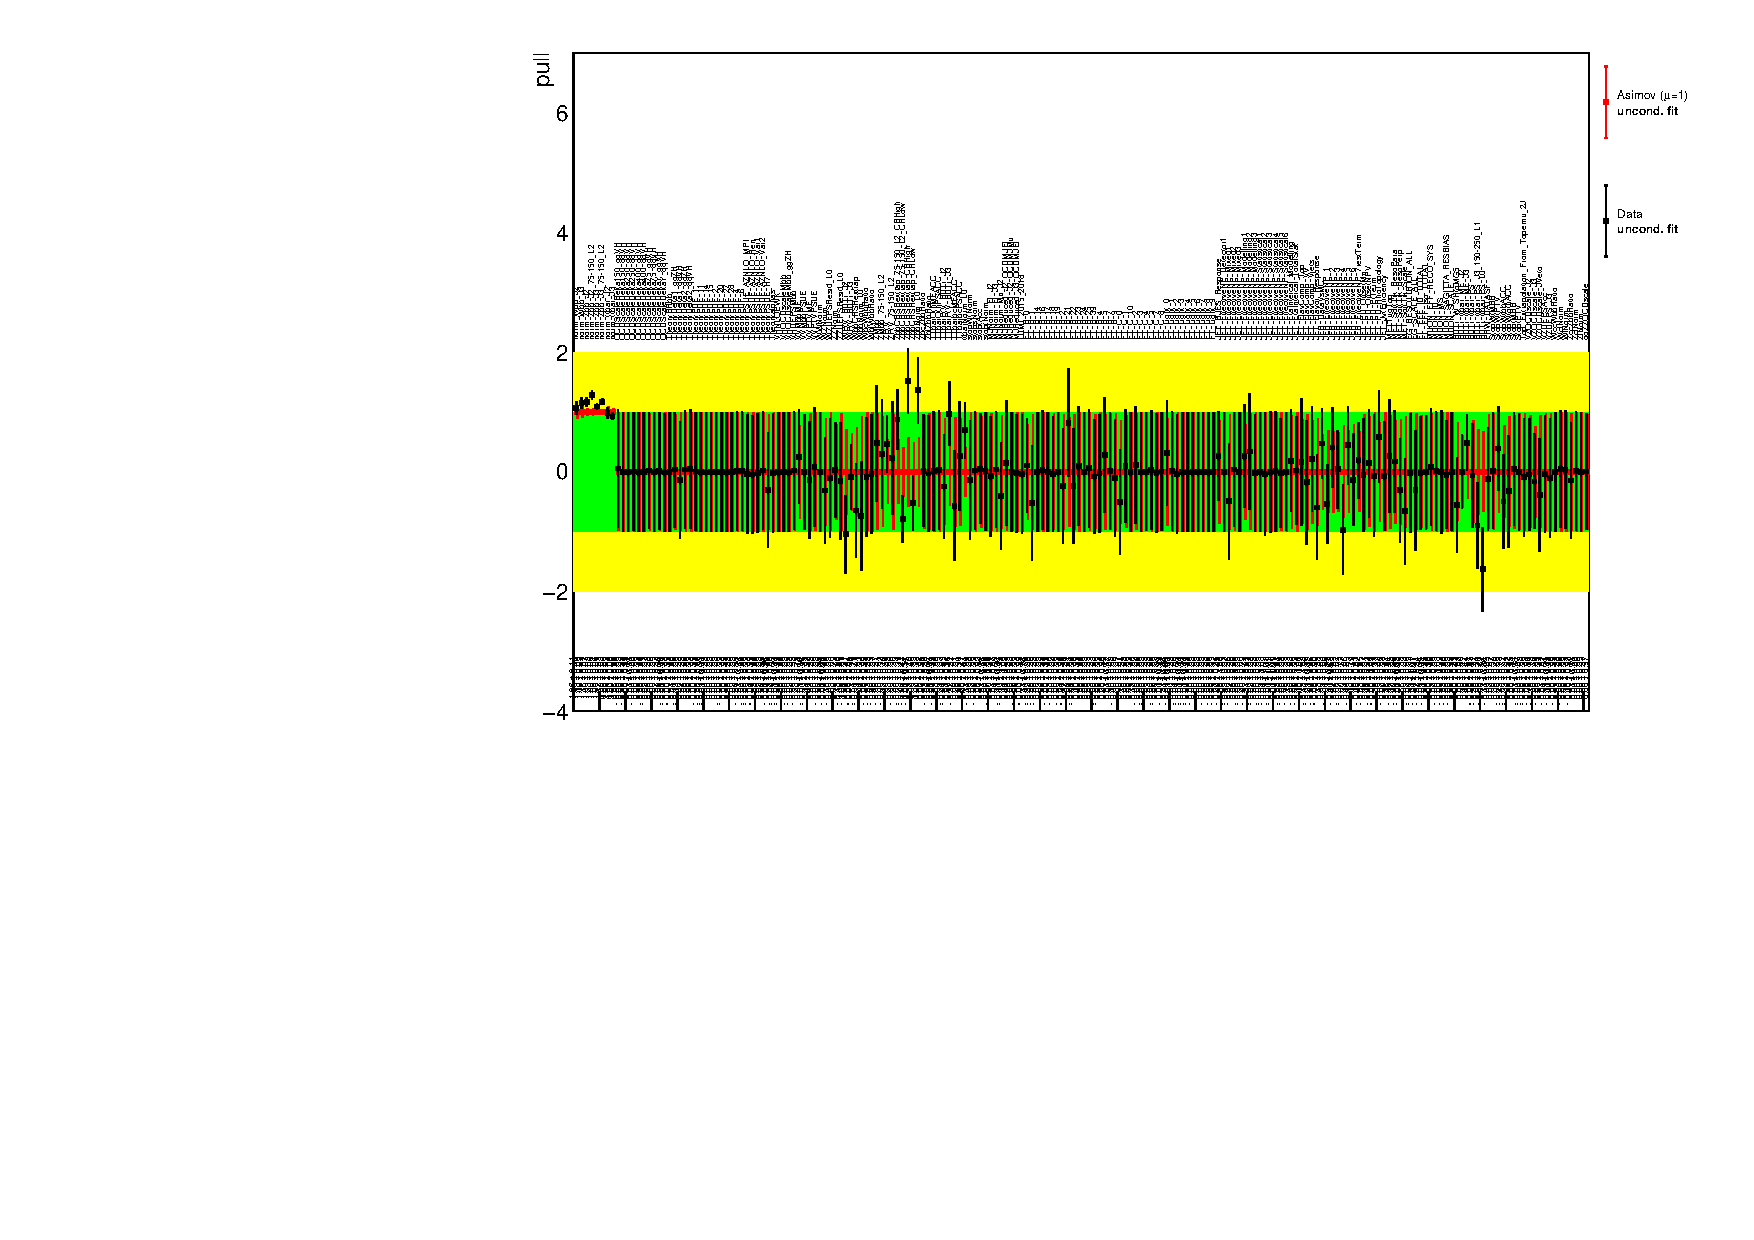
\includegraphics[angle=270]{final_fit_mva/pullComparisons/NP_allExceptGammas.pdf}
% \caption{caption}
% % Nuisance parameter pulls and the free parameter scale factors corresponding to
% % an unconditional combined fit performed to the Asimov dataset (red) and an
% % unconditional combined fit to the \RunTwo data (black).
% \label{fig:nppulls_012L_MVAVH} 
% \end{figure}
%
\begin{figure}[hb]
\centering
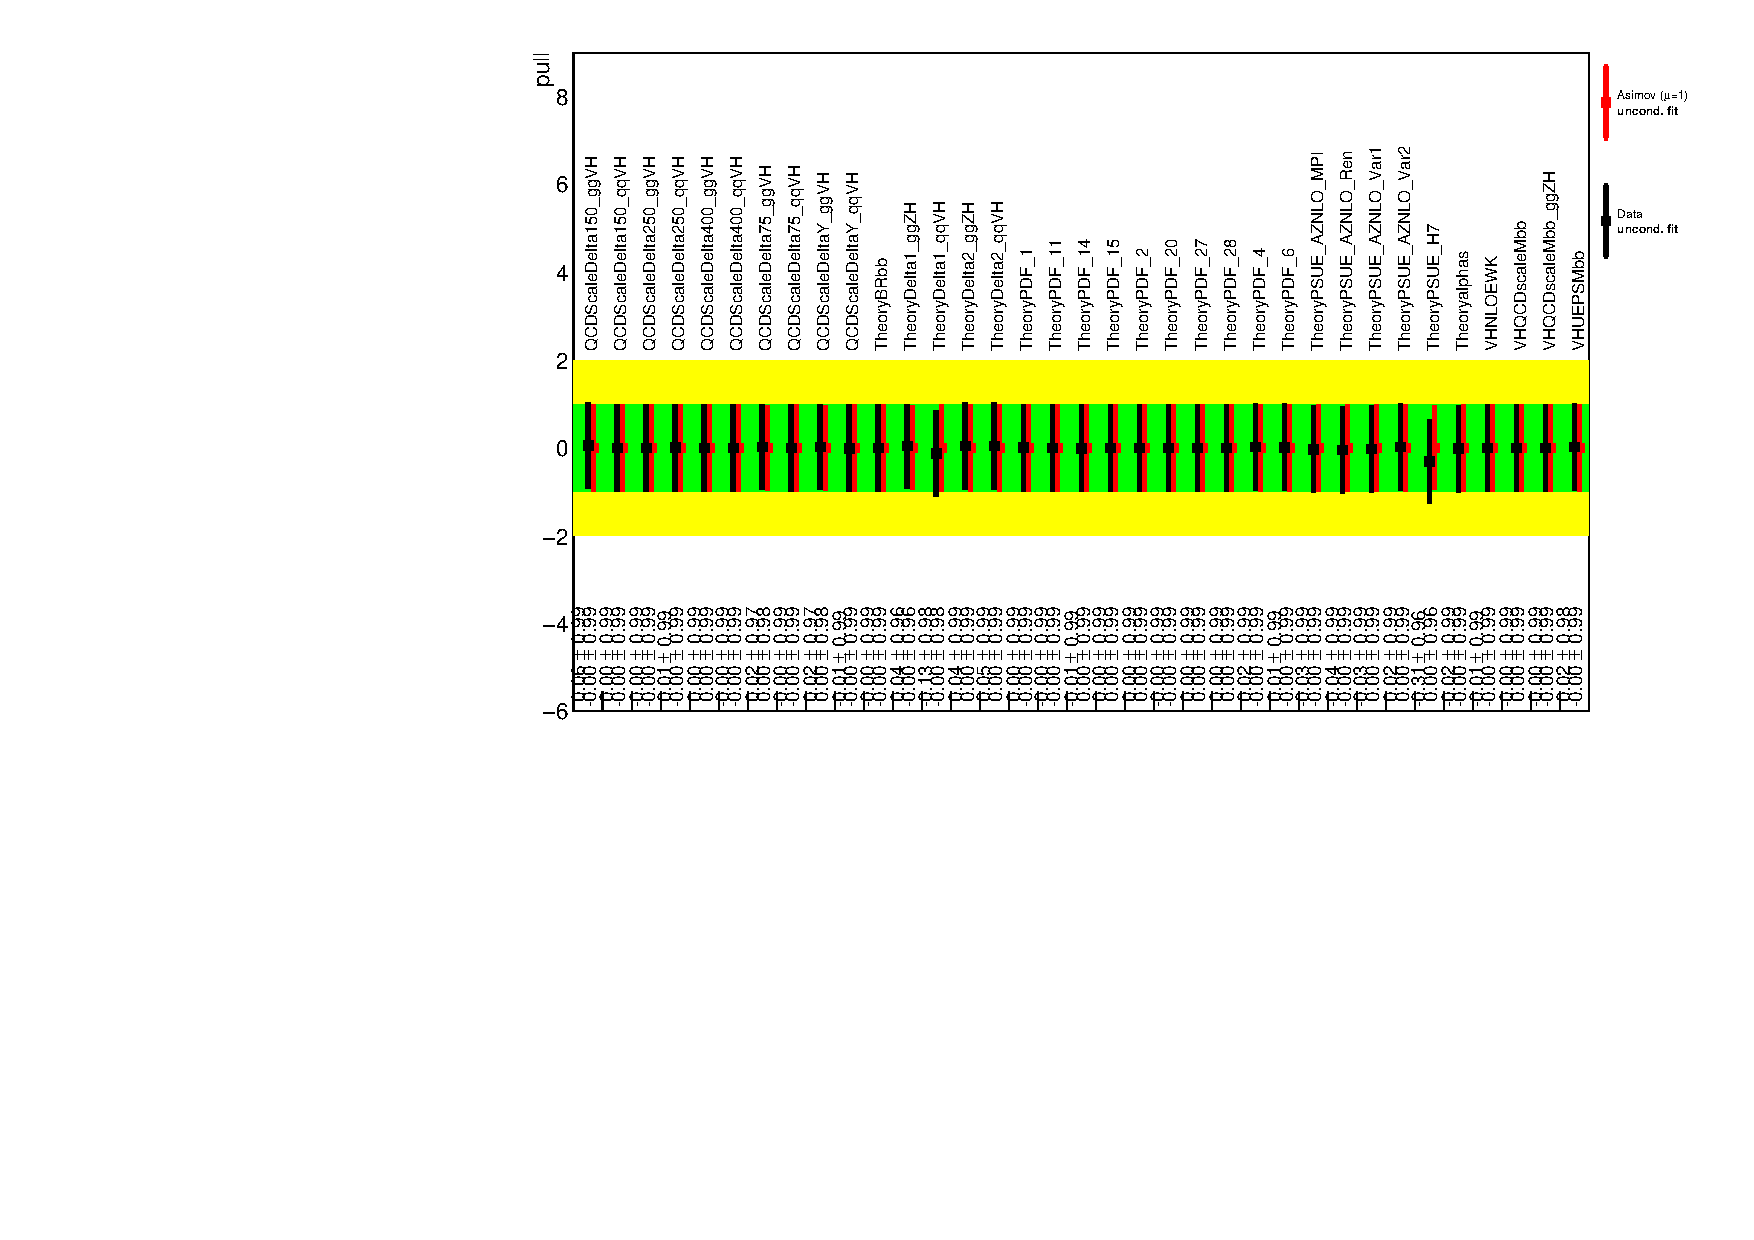
\includegraphics[width=0.49\linewidth]{final_fit_mva/pullComparisons/NP_VH.pdf}
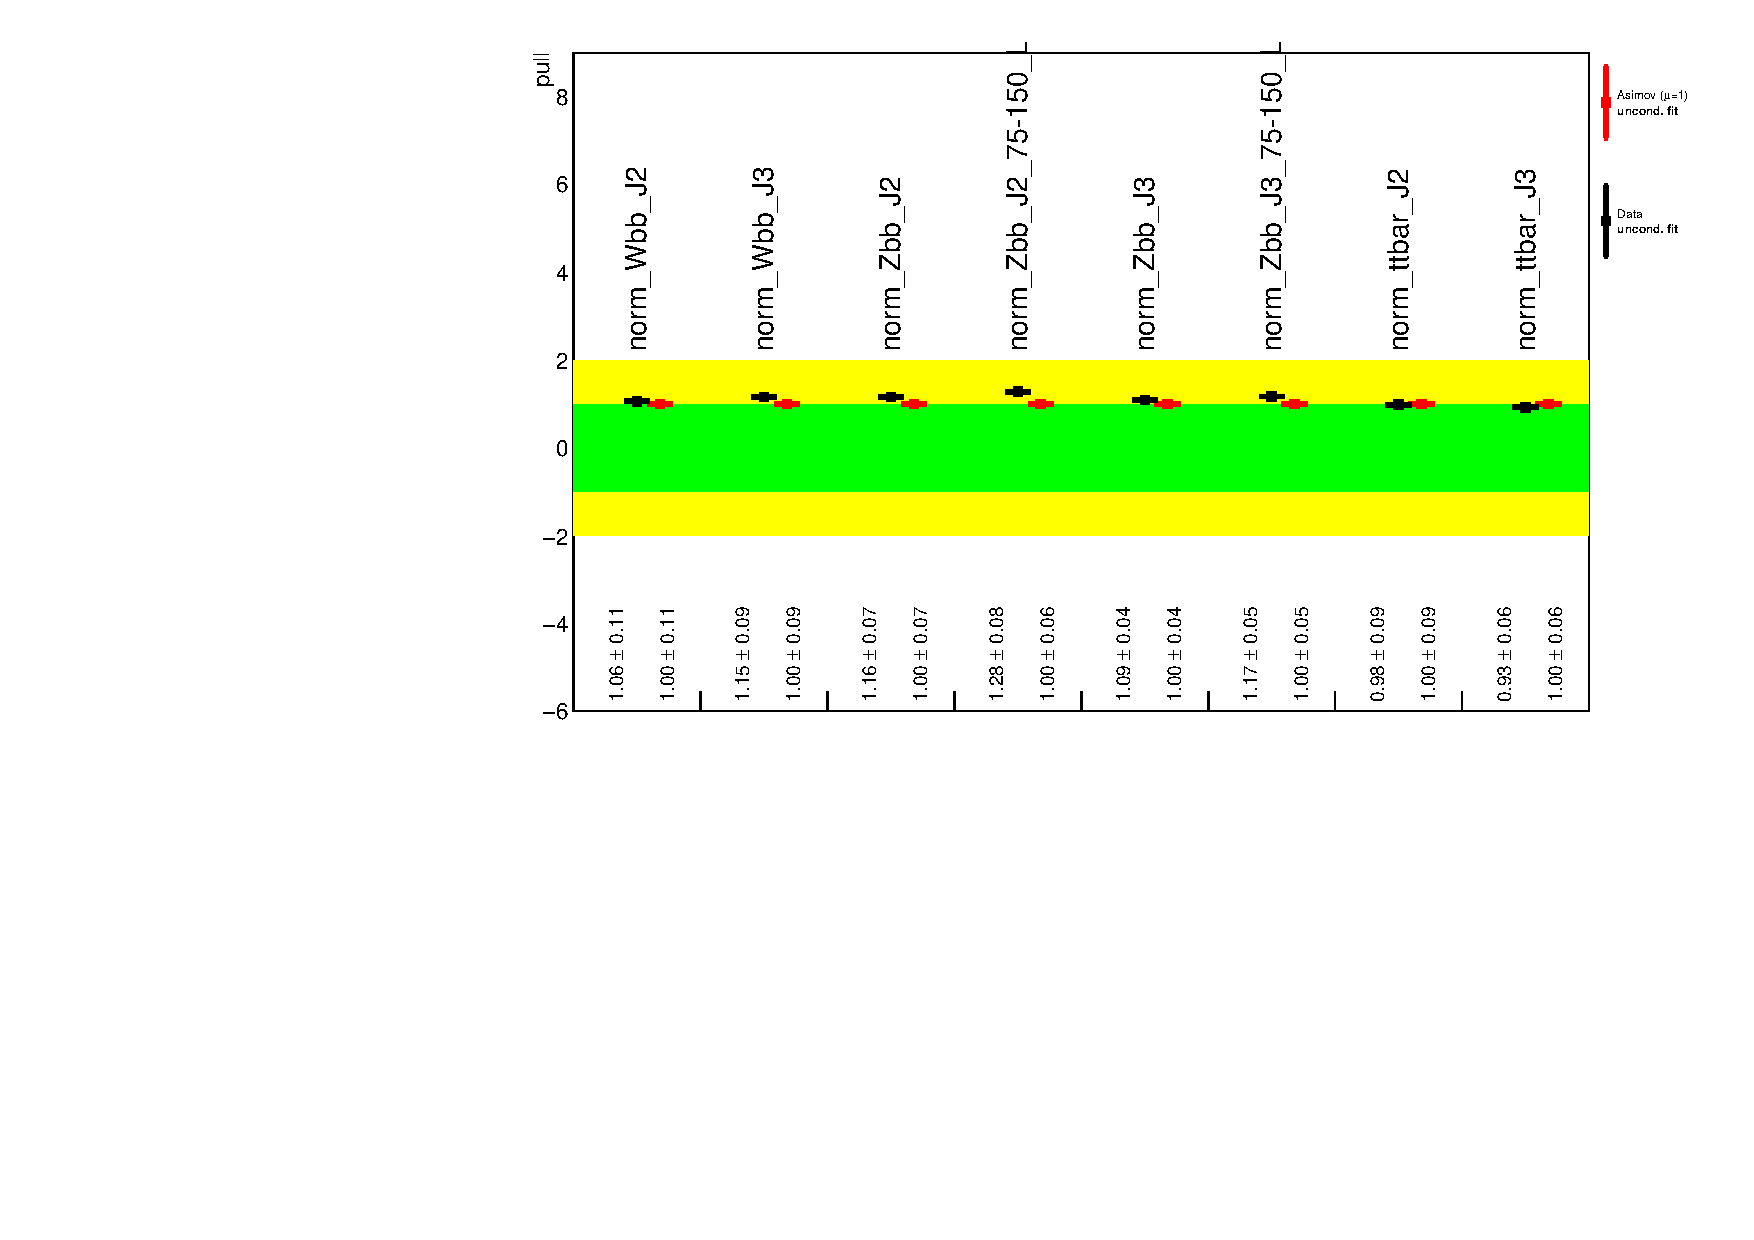
\includegraphics[width=0.49\linewidth]{final_fit_mva/pullComparisons/NP_FloatNorm.pdf}
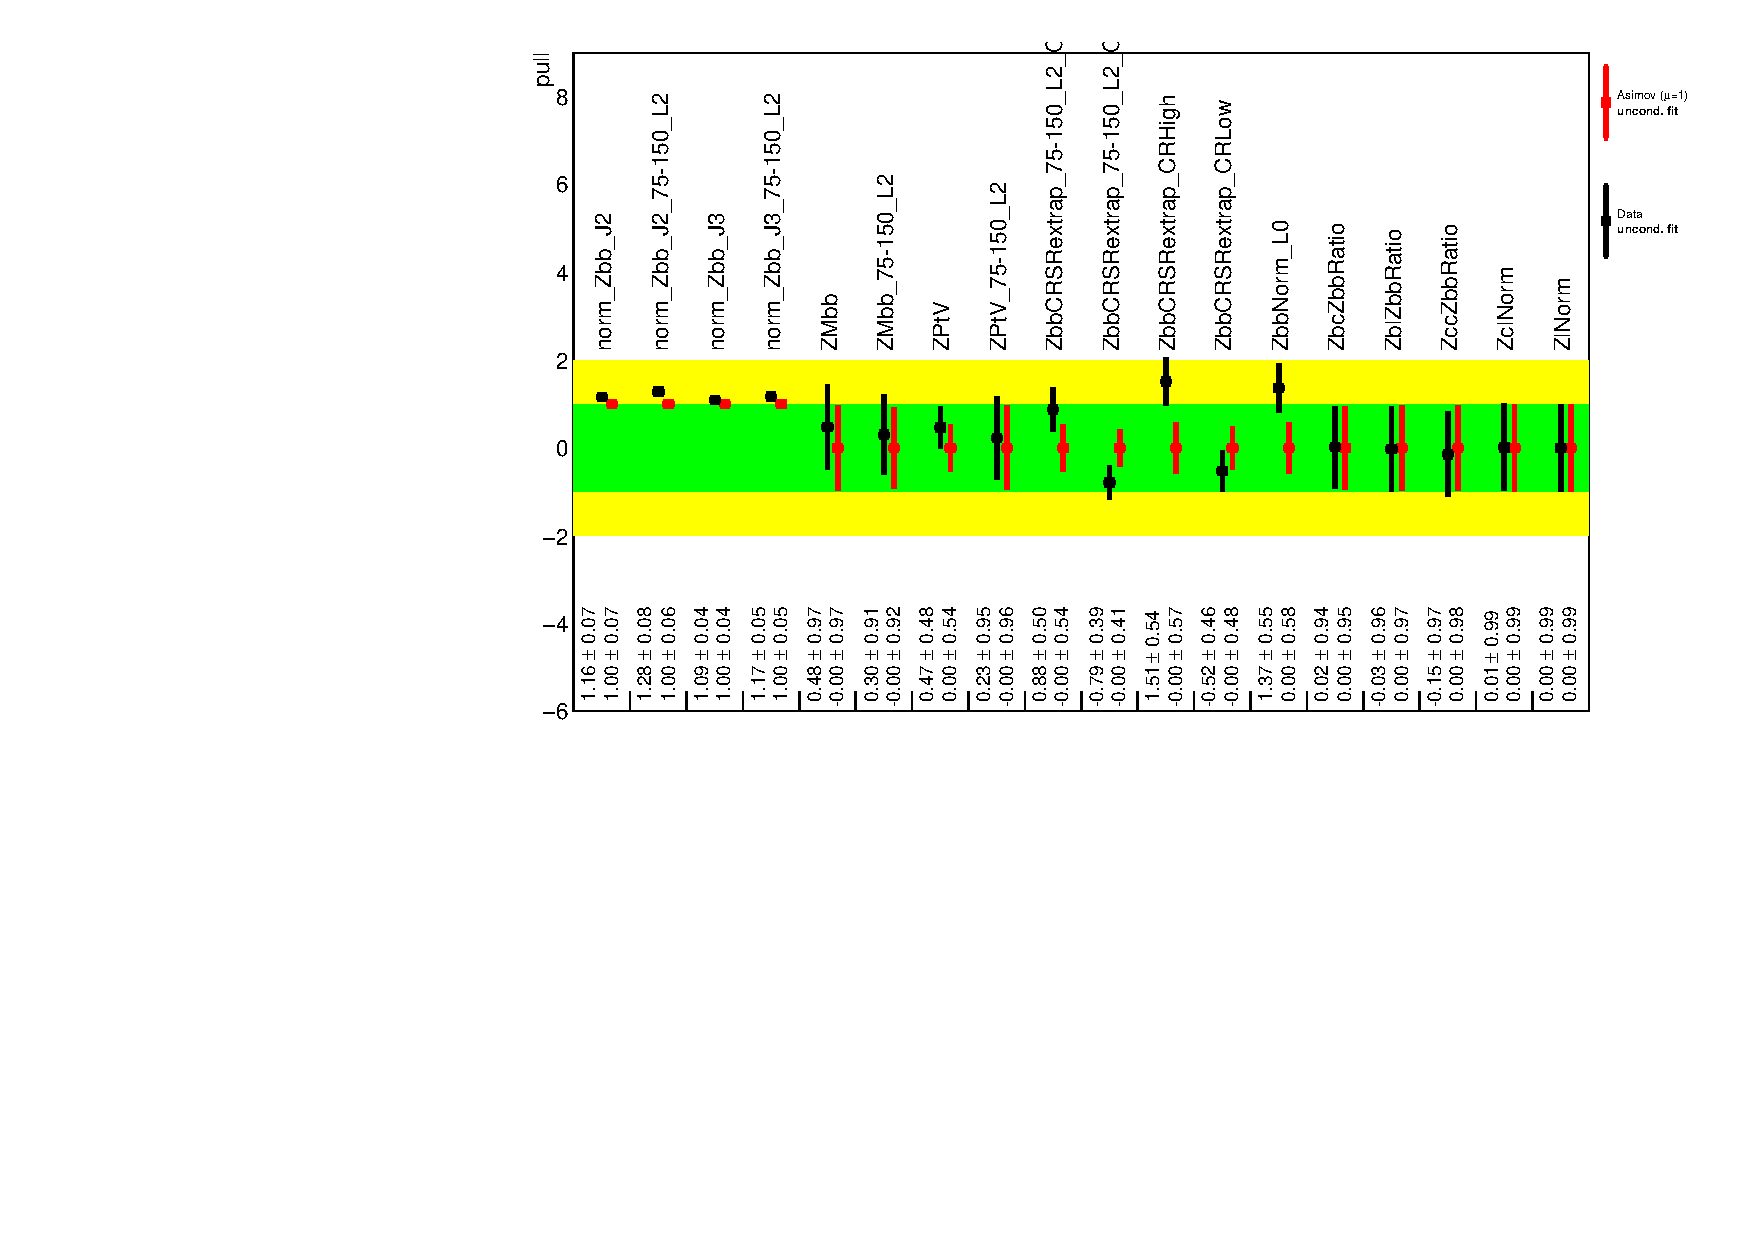
\includegraphics[width=0.49\linewidth]{final_fit_mva/pullComparisons/NP_Zjets.pdf}
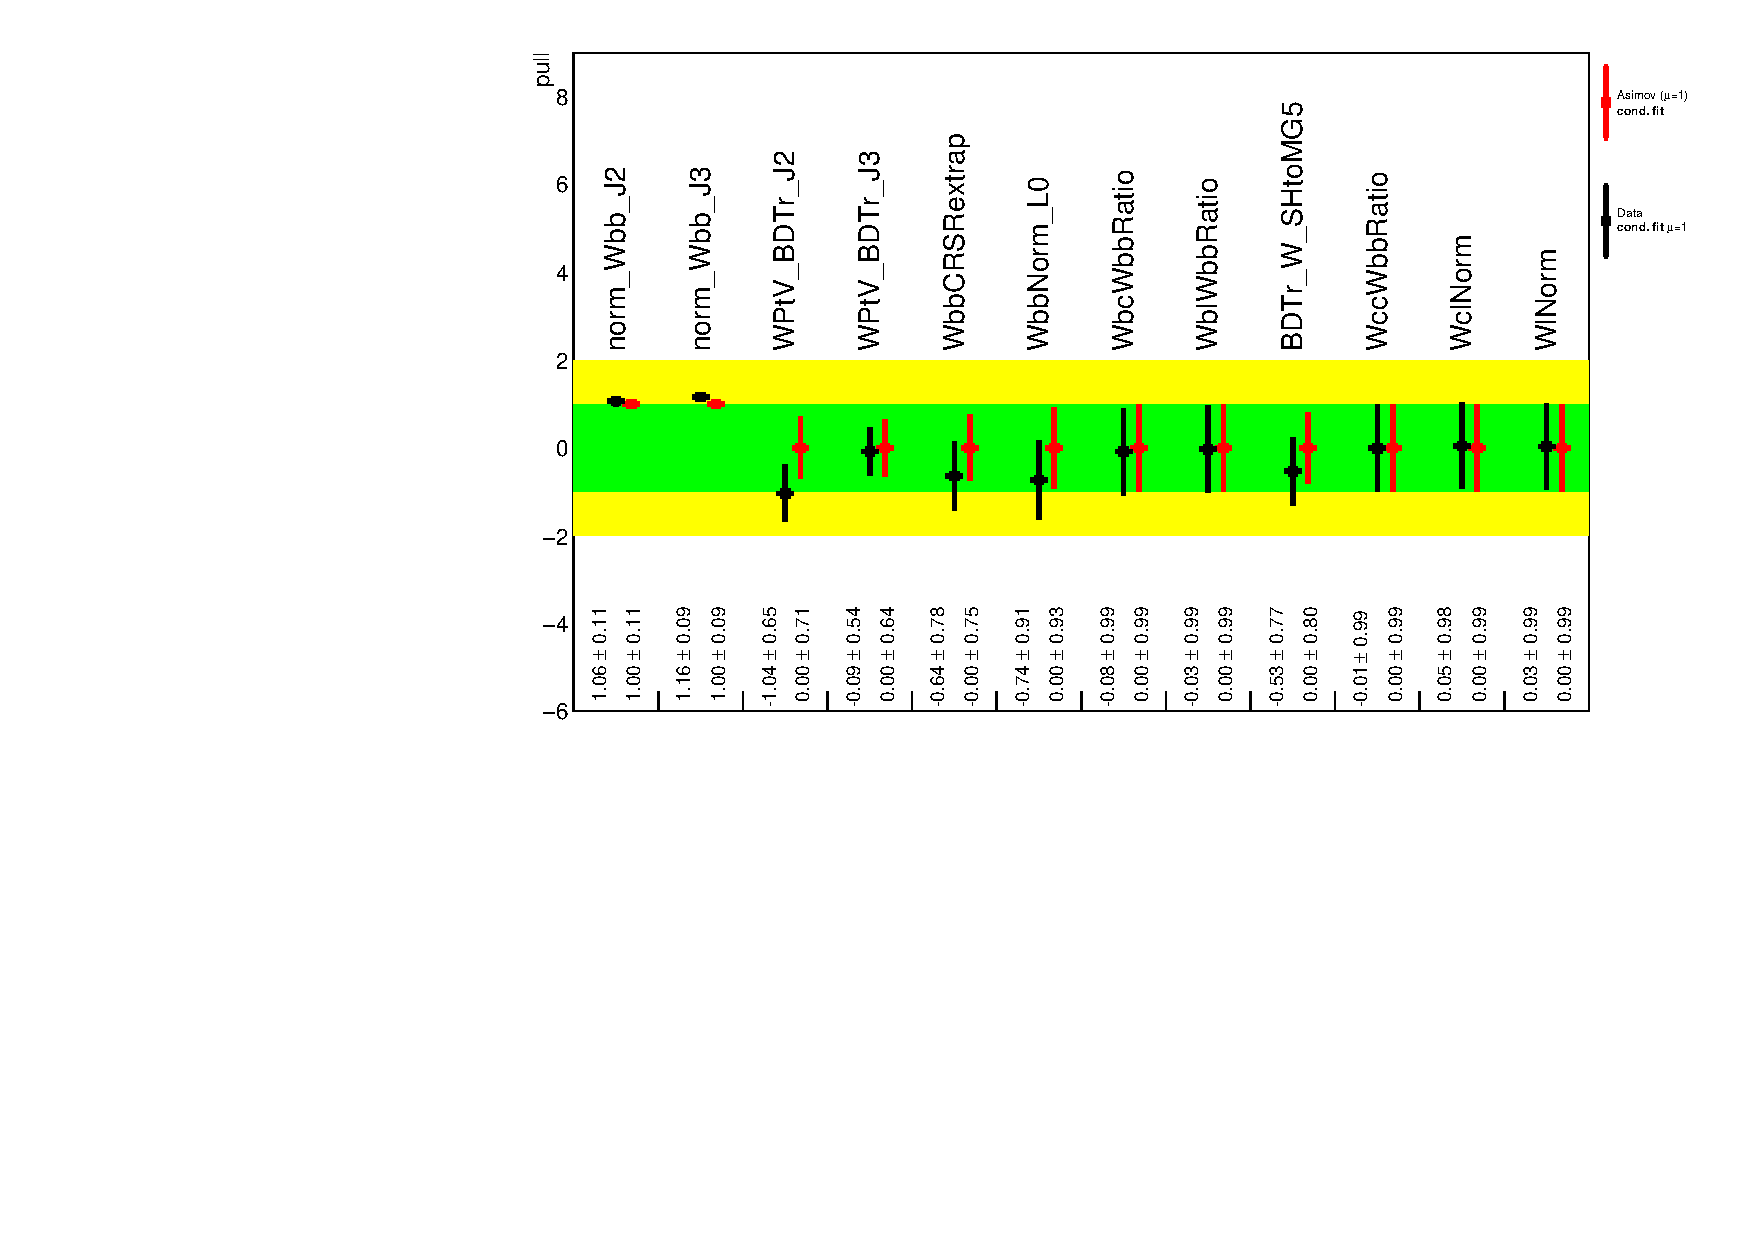
\includegraphics[width=0.49\linewidth]{final_fit_mva/pullComparisons/NP_Wjets.pdf}
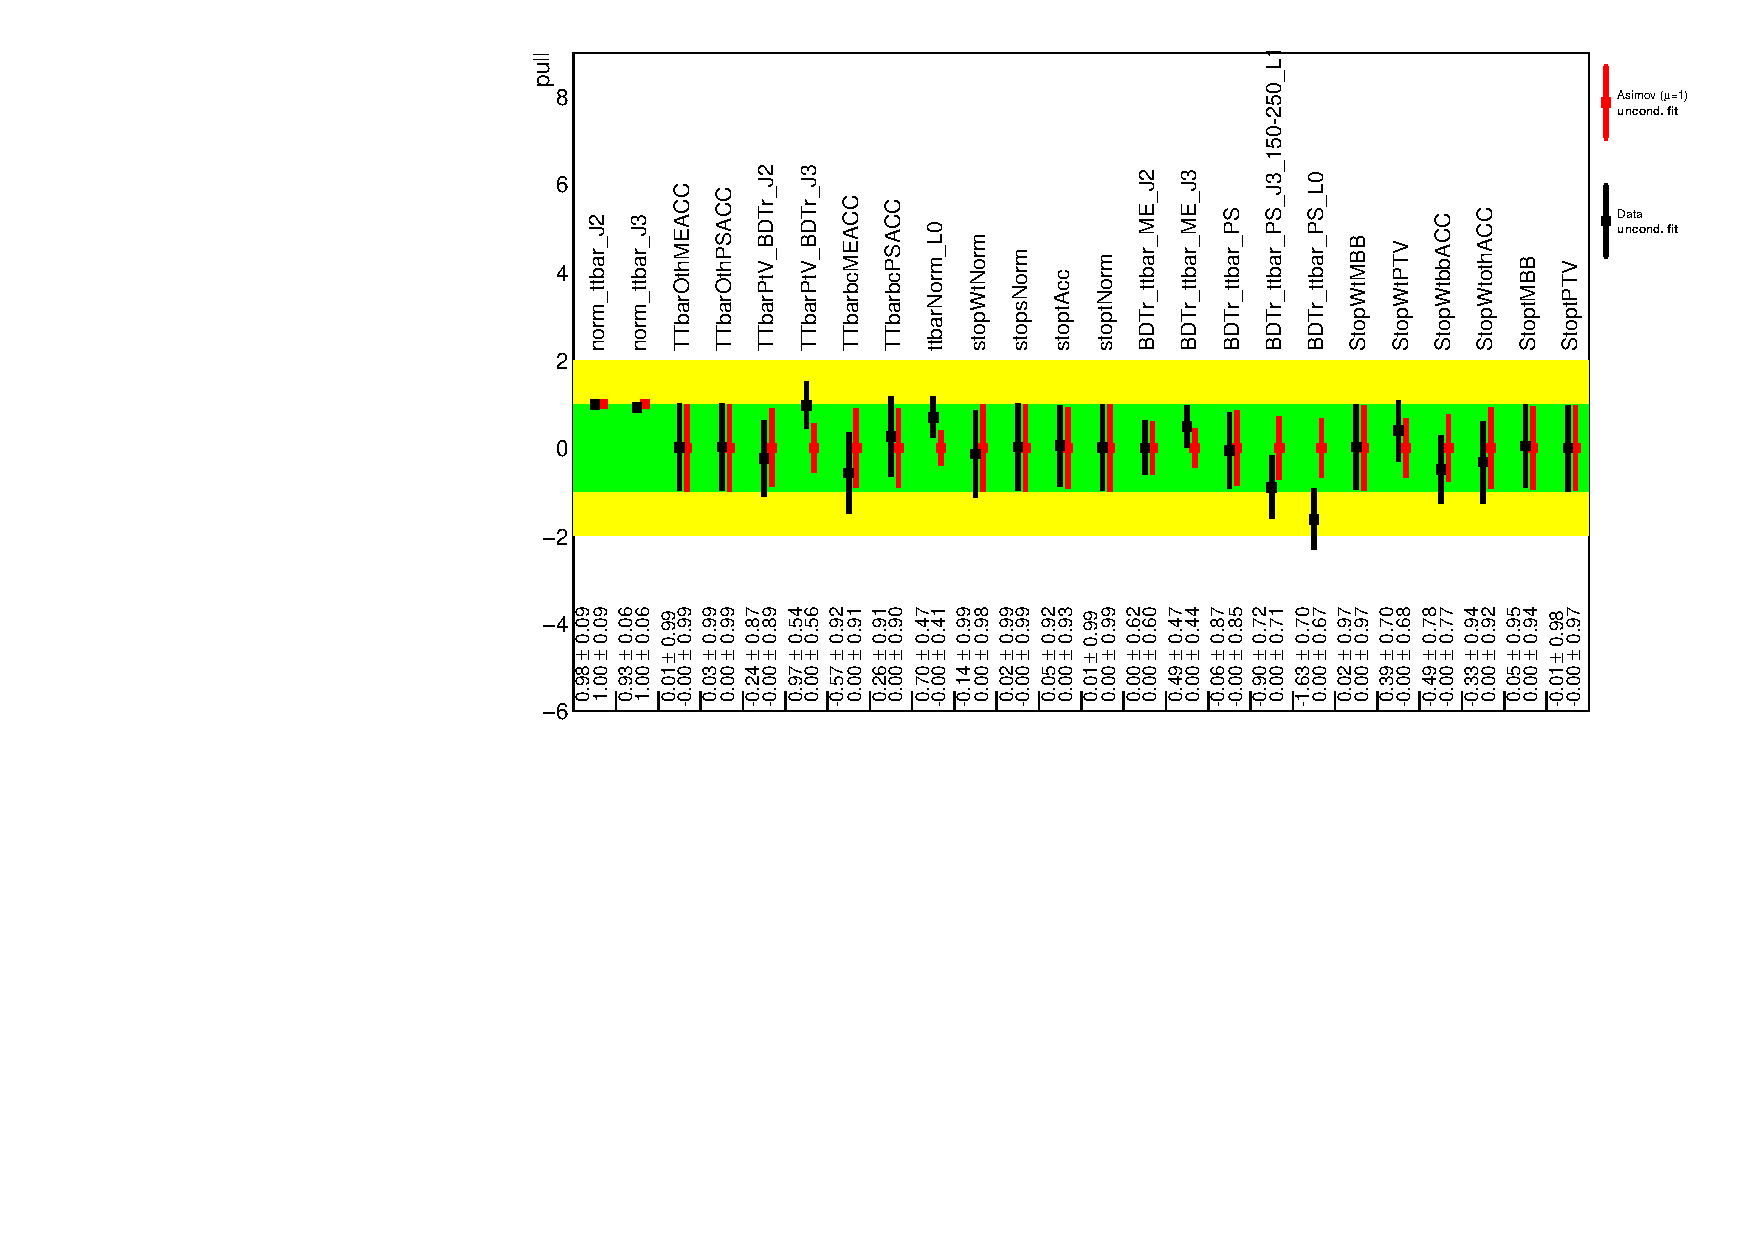
\includegraphics[width=0.49\linewidth]{final_fit_mva/pullComparisons/NP_Top.pdf}
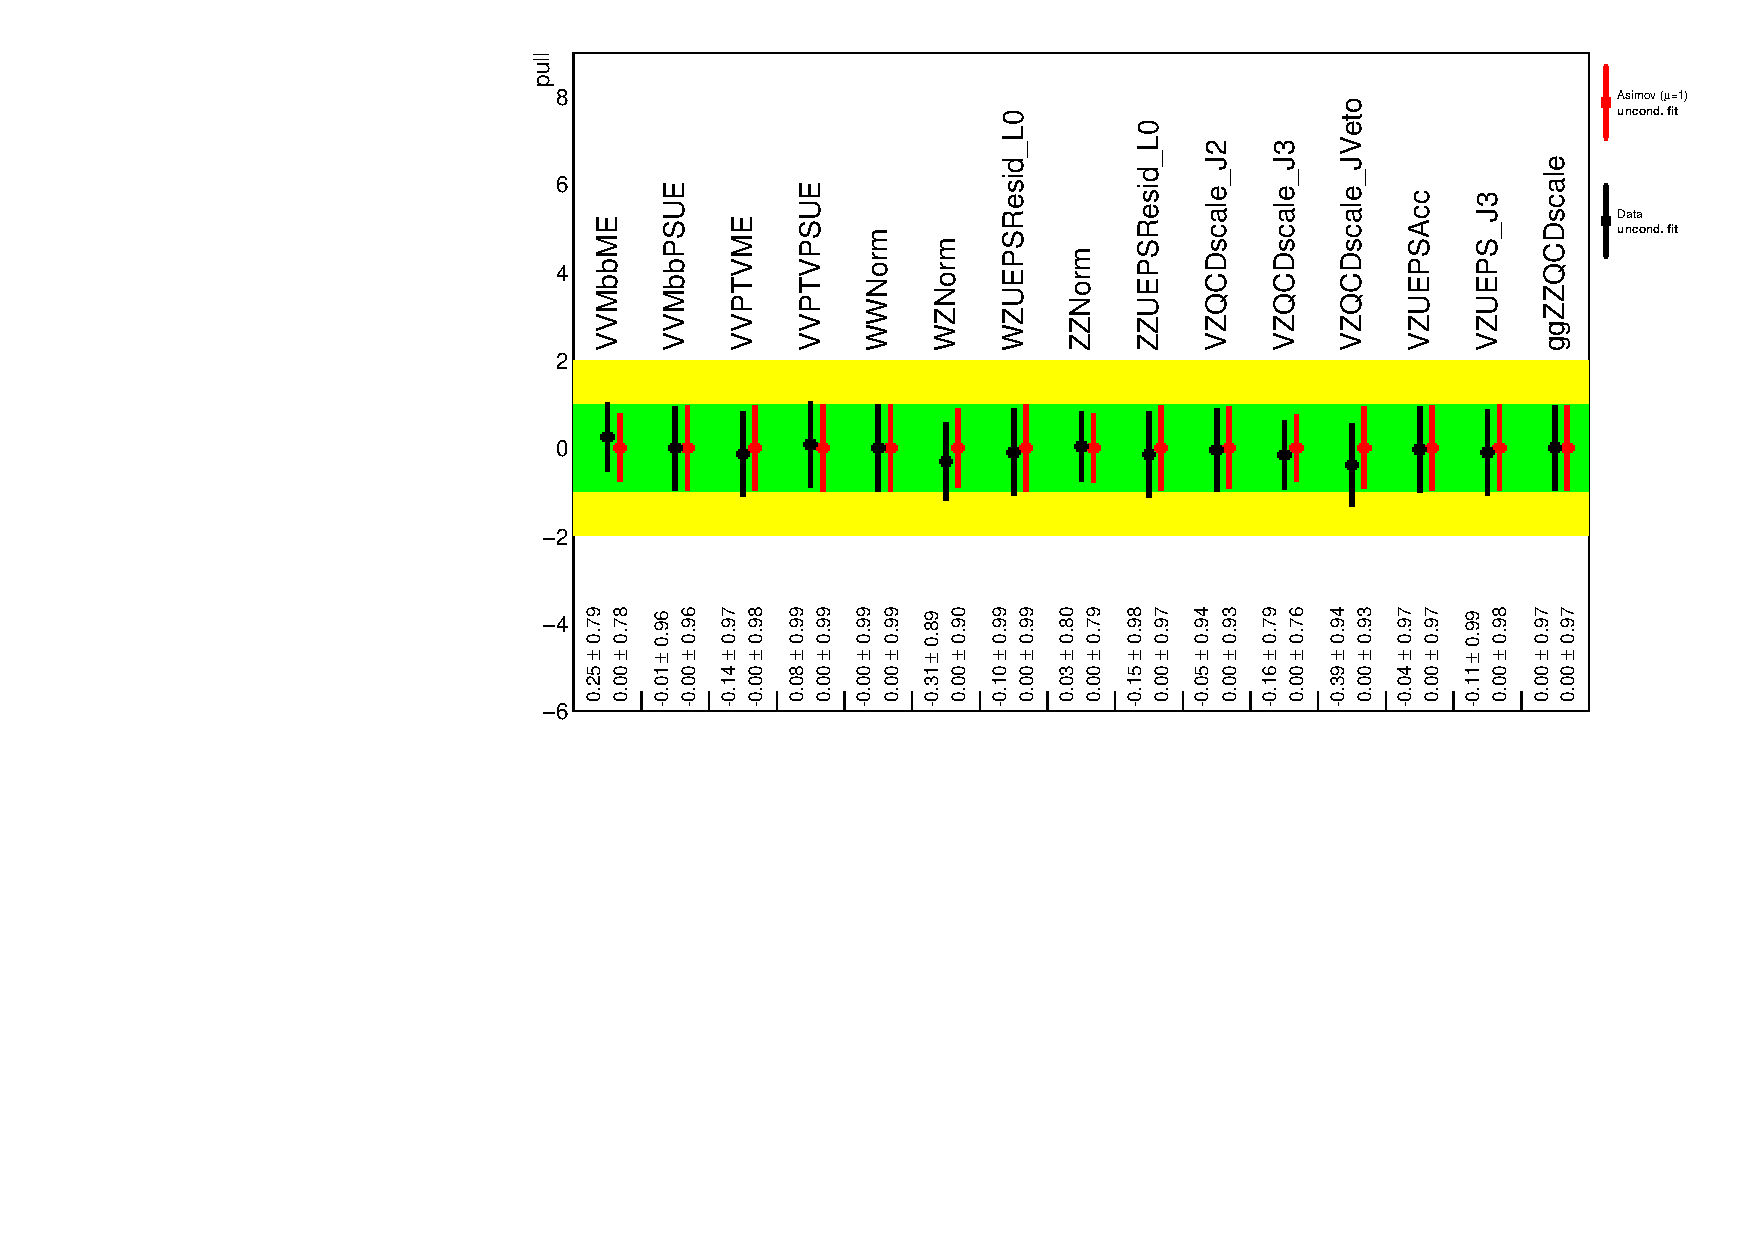
\includegraphics[width=0.49\linewidth]{final_fit_mva/pullComparisons/NP_Diboson.pdf}
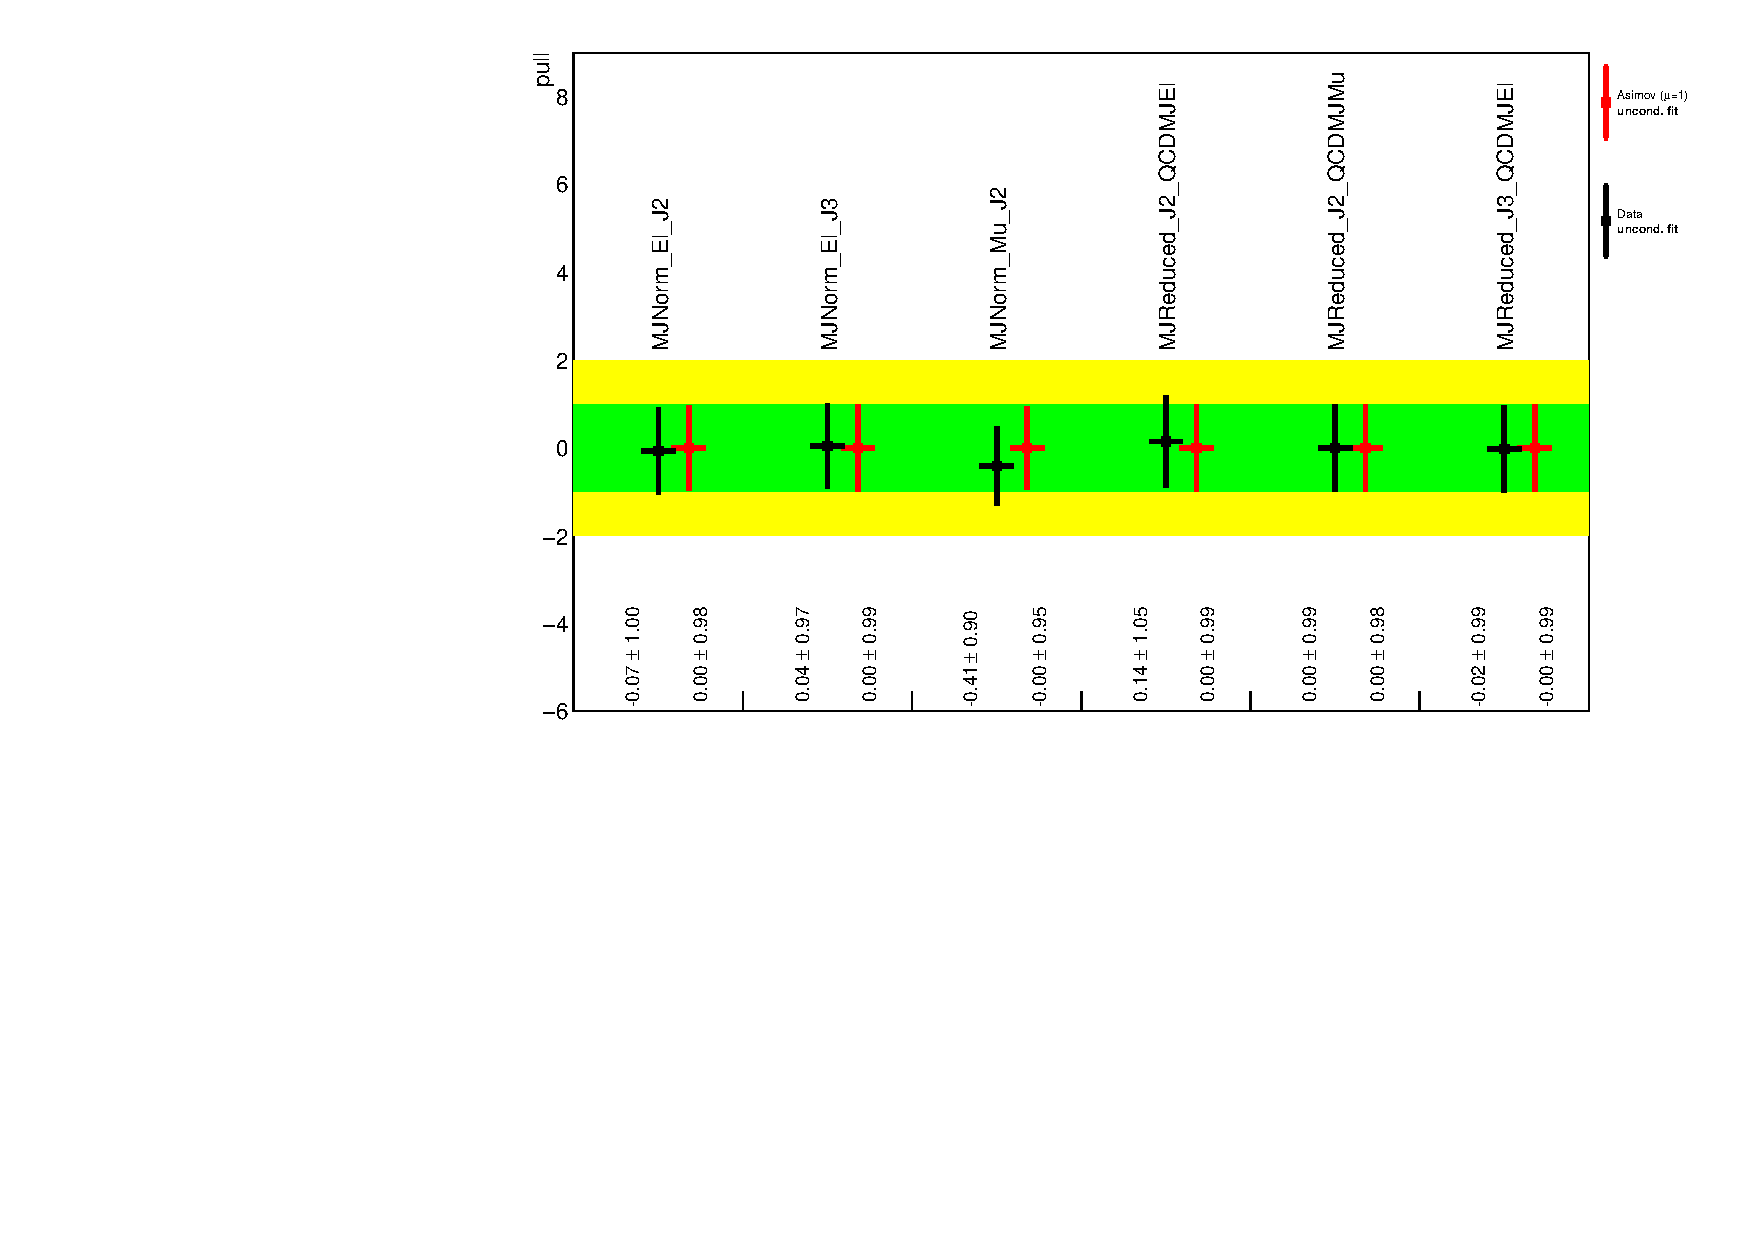
\includegraphics[width=0.49\linewidth]{final_fit_mva/pullComparisons/NP_MJ.pdf}
\caption{caption}
% MC modelling, multi-jet estimate nuisance parameter pulls and the free parameter
% scale factors corresponding to a conditional combined fit performed to Asimov
% dataset (red) and an unconditional combined fit to the \RunTwo data (black).
\label{fig:nppulls_012L_MVAVH_a} 
\end{figure}
%
\begin{figure}[hb]
\centering
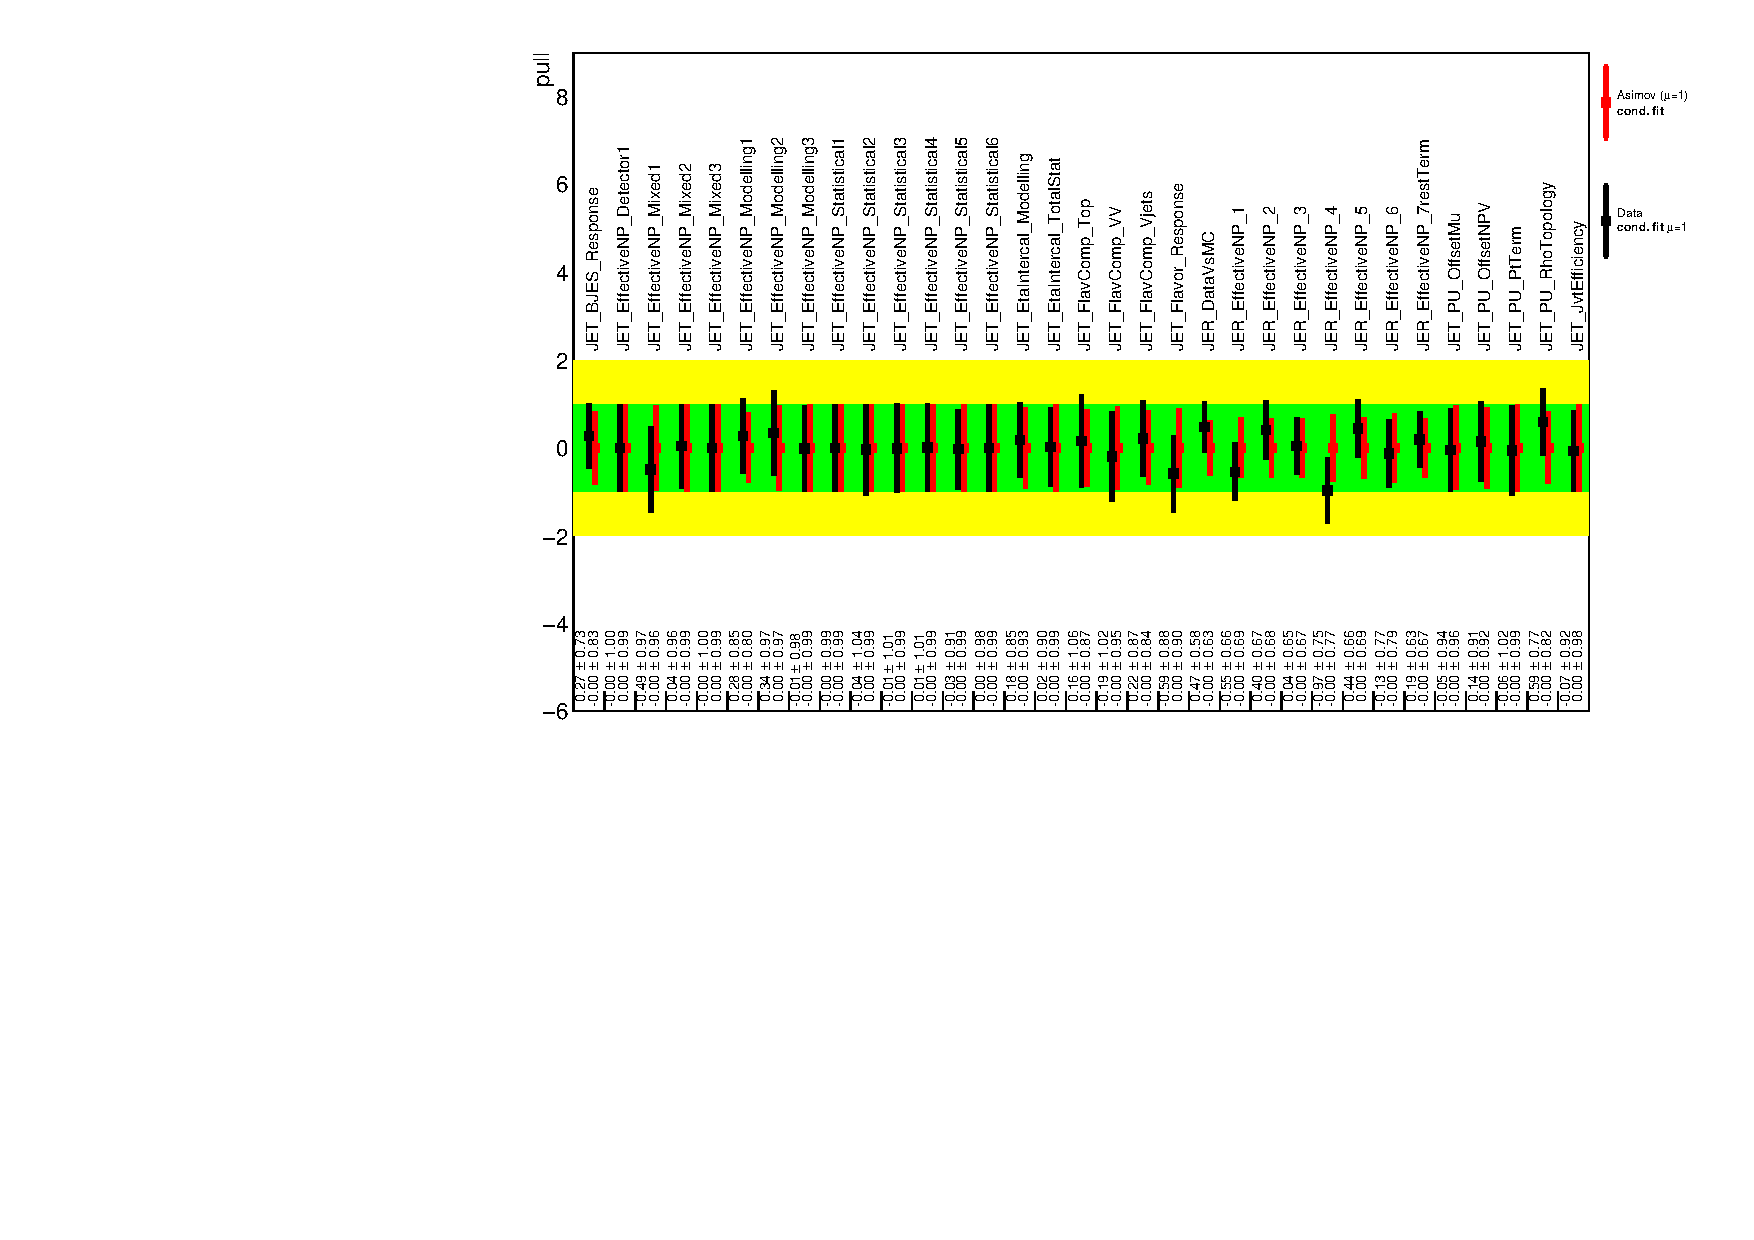
\includegraphics[width=0.49\linewidth]{final_fit_mva/pullComparisons/NP_Jet.pdf}
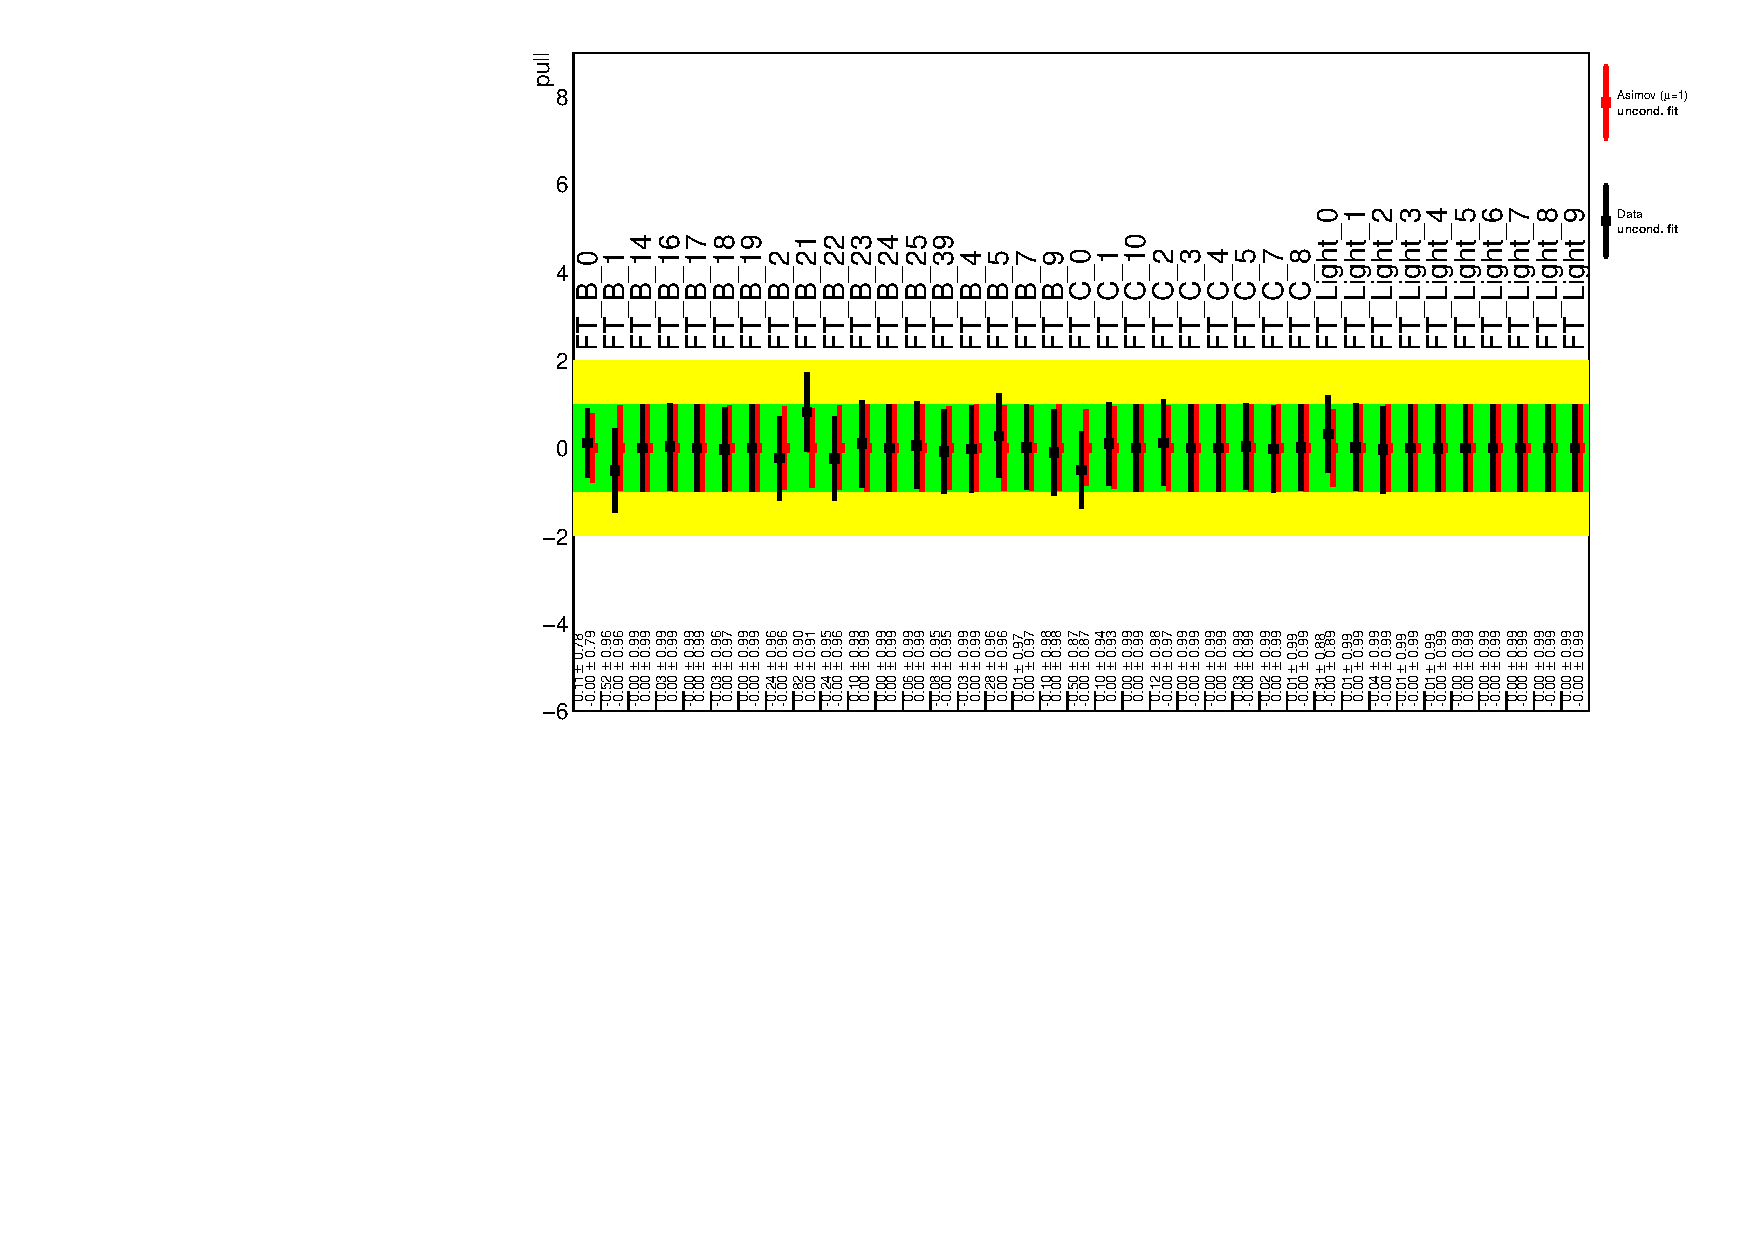
\includegraphics[width=0.49\linewidth]{final_fit_mva/pullComparisons/NP_BTag.pdf}
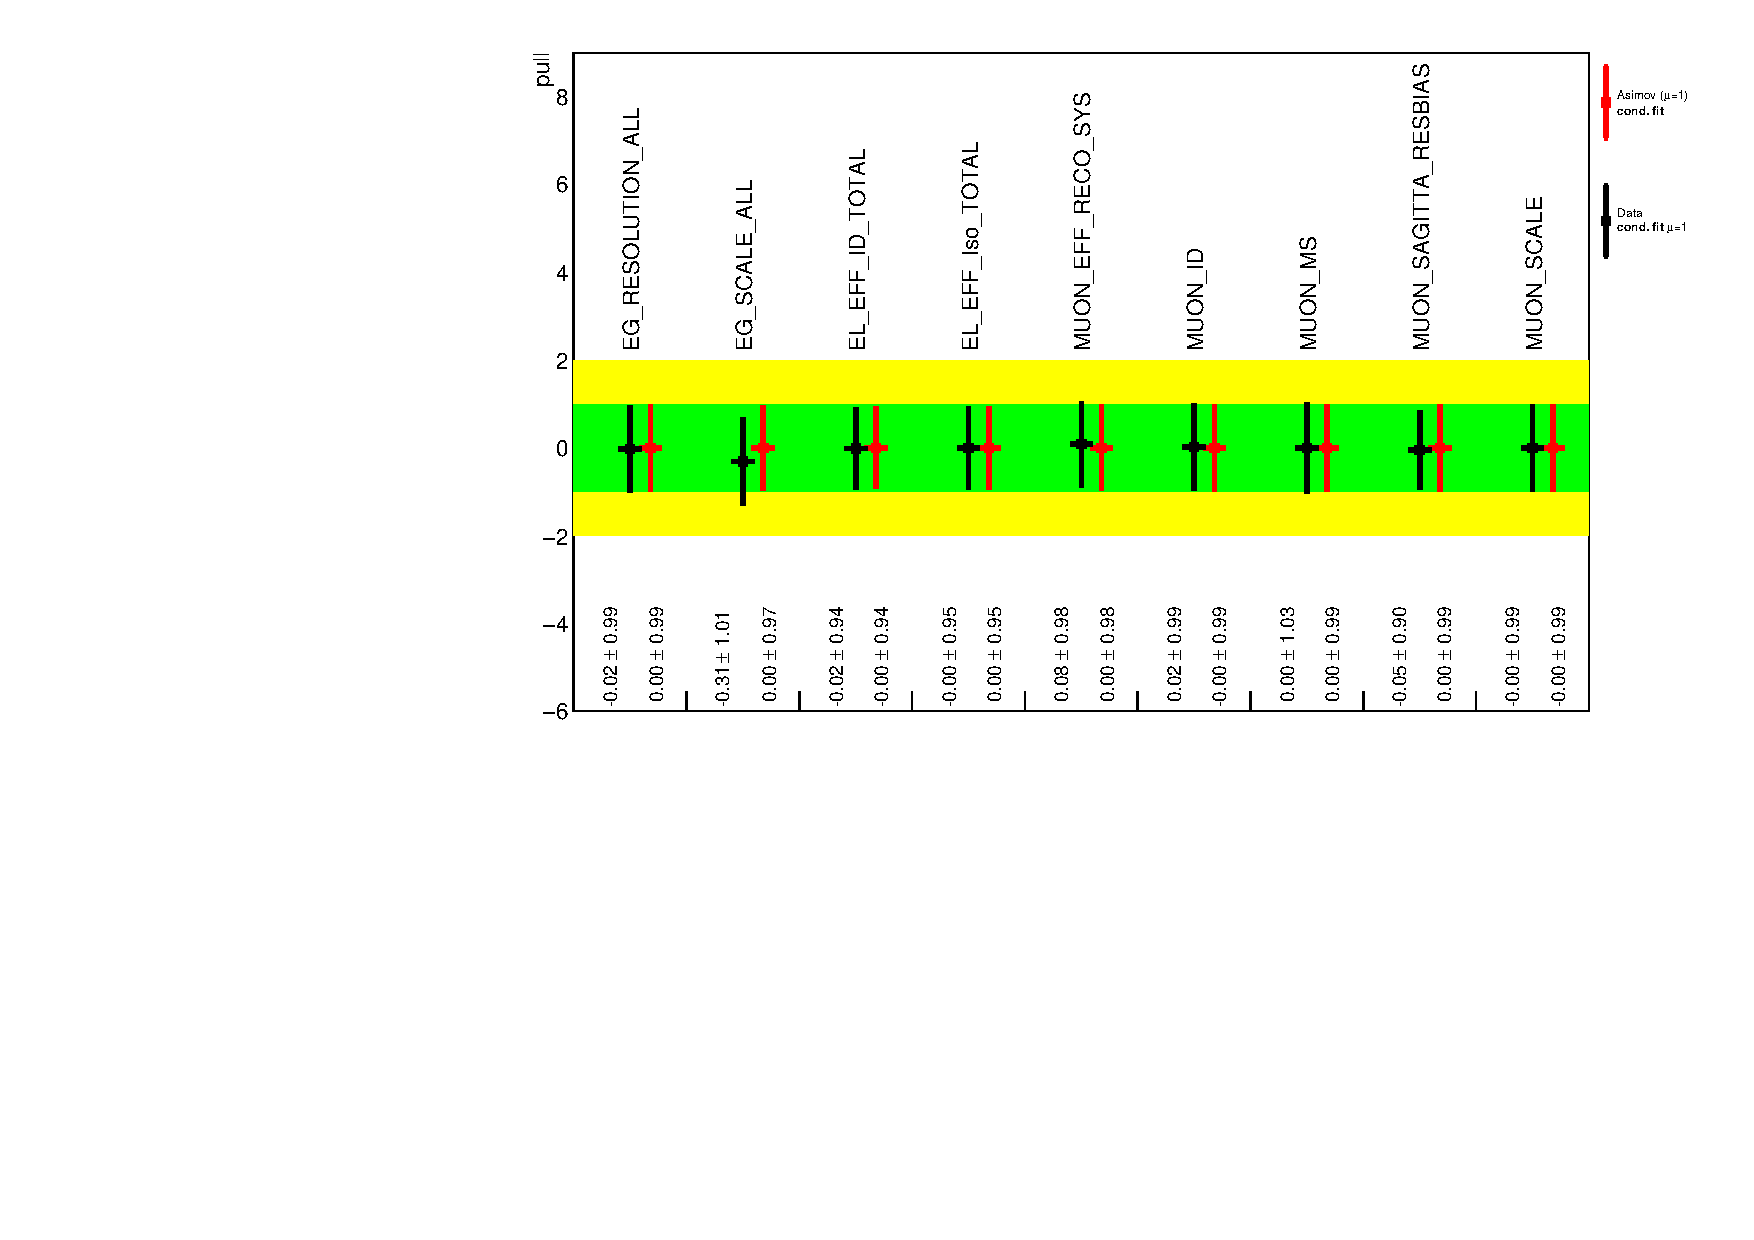
\includegraphics[width=0.49\linewidth]{final_fit_mva/pullComparisons/NP_Lepton.pdf}
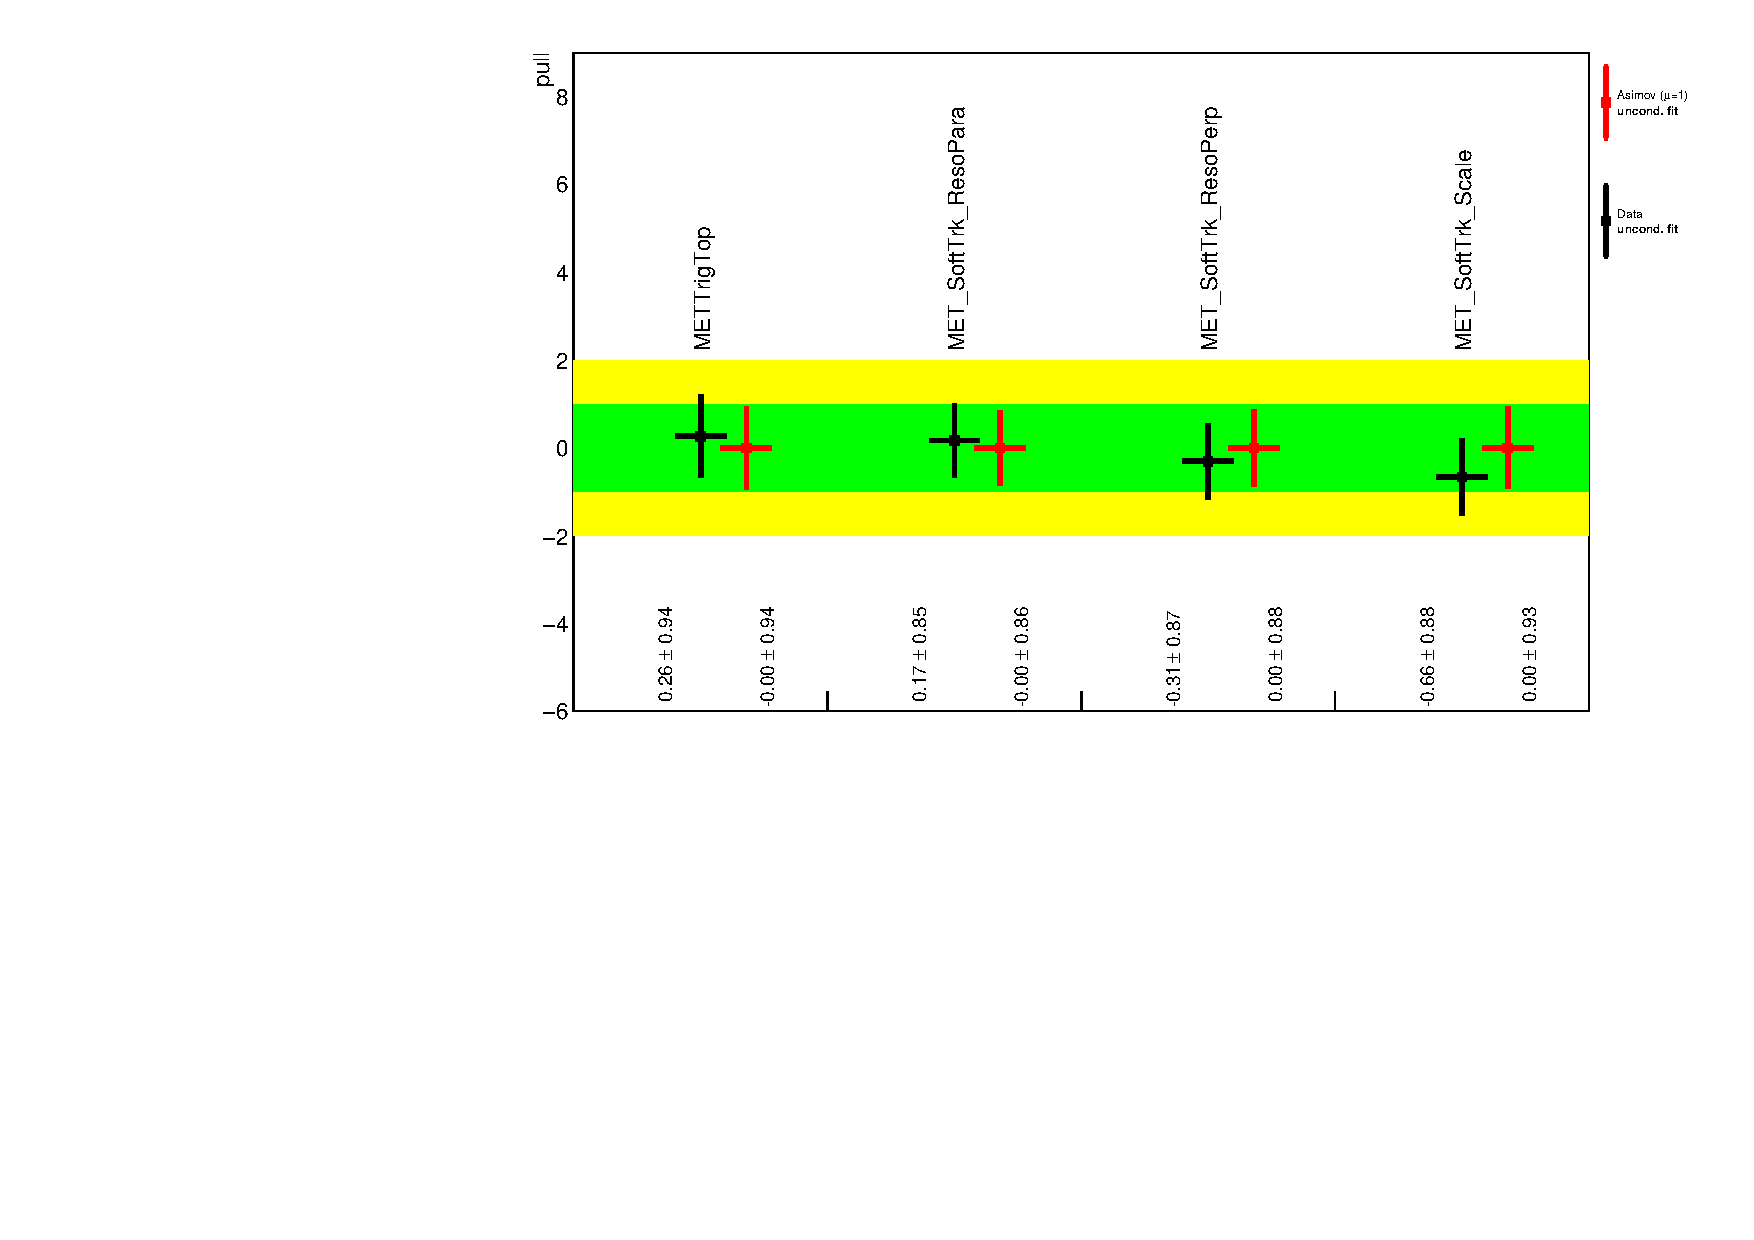
\includegraphics[width=0.49\linewidth]{final_fit_mva/pullComparisons/NP_MET.pdf}
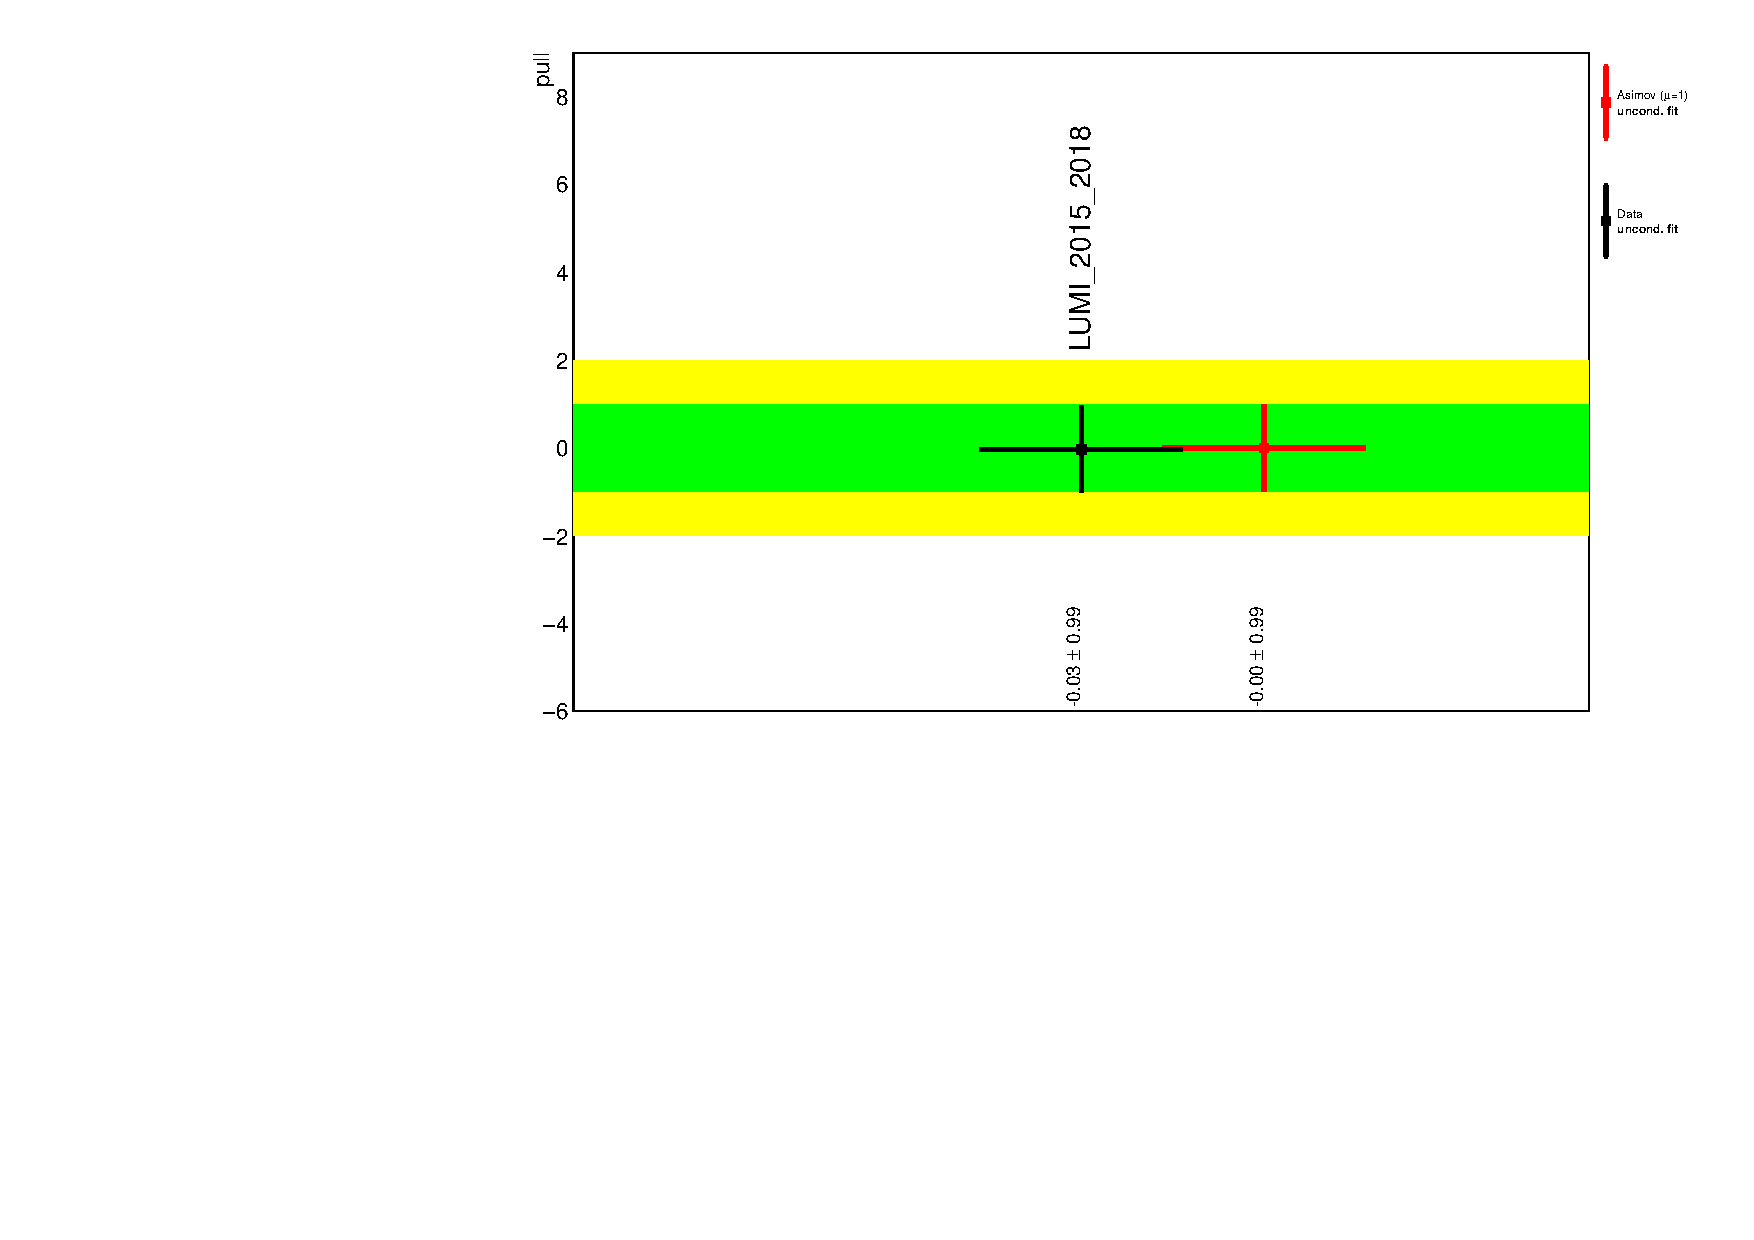
\includegraphics[width=0.49\linewidth]{final_fit_mva/pullComparisons/NP_LUMI.pdf}
\caption{caption}
% Detector and luminosity nuisance parameter pulls corresponding to a conditional
% combined fit performed to an Asimov dataset (red) and an unconditional combined
% fit to the \RunTwo data (black)
\label{fig:nppulls_012L_MVAVH_b}
\end{figure}
%
% \begin{figure}[hb]
% \centering
% 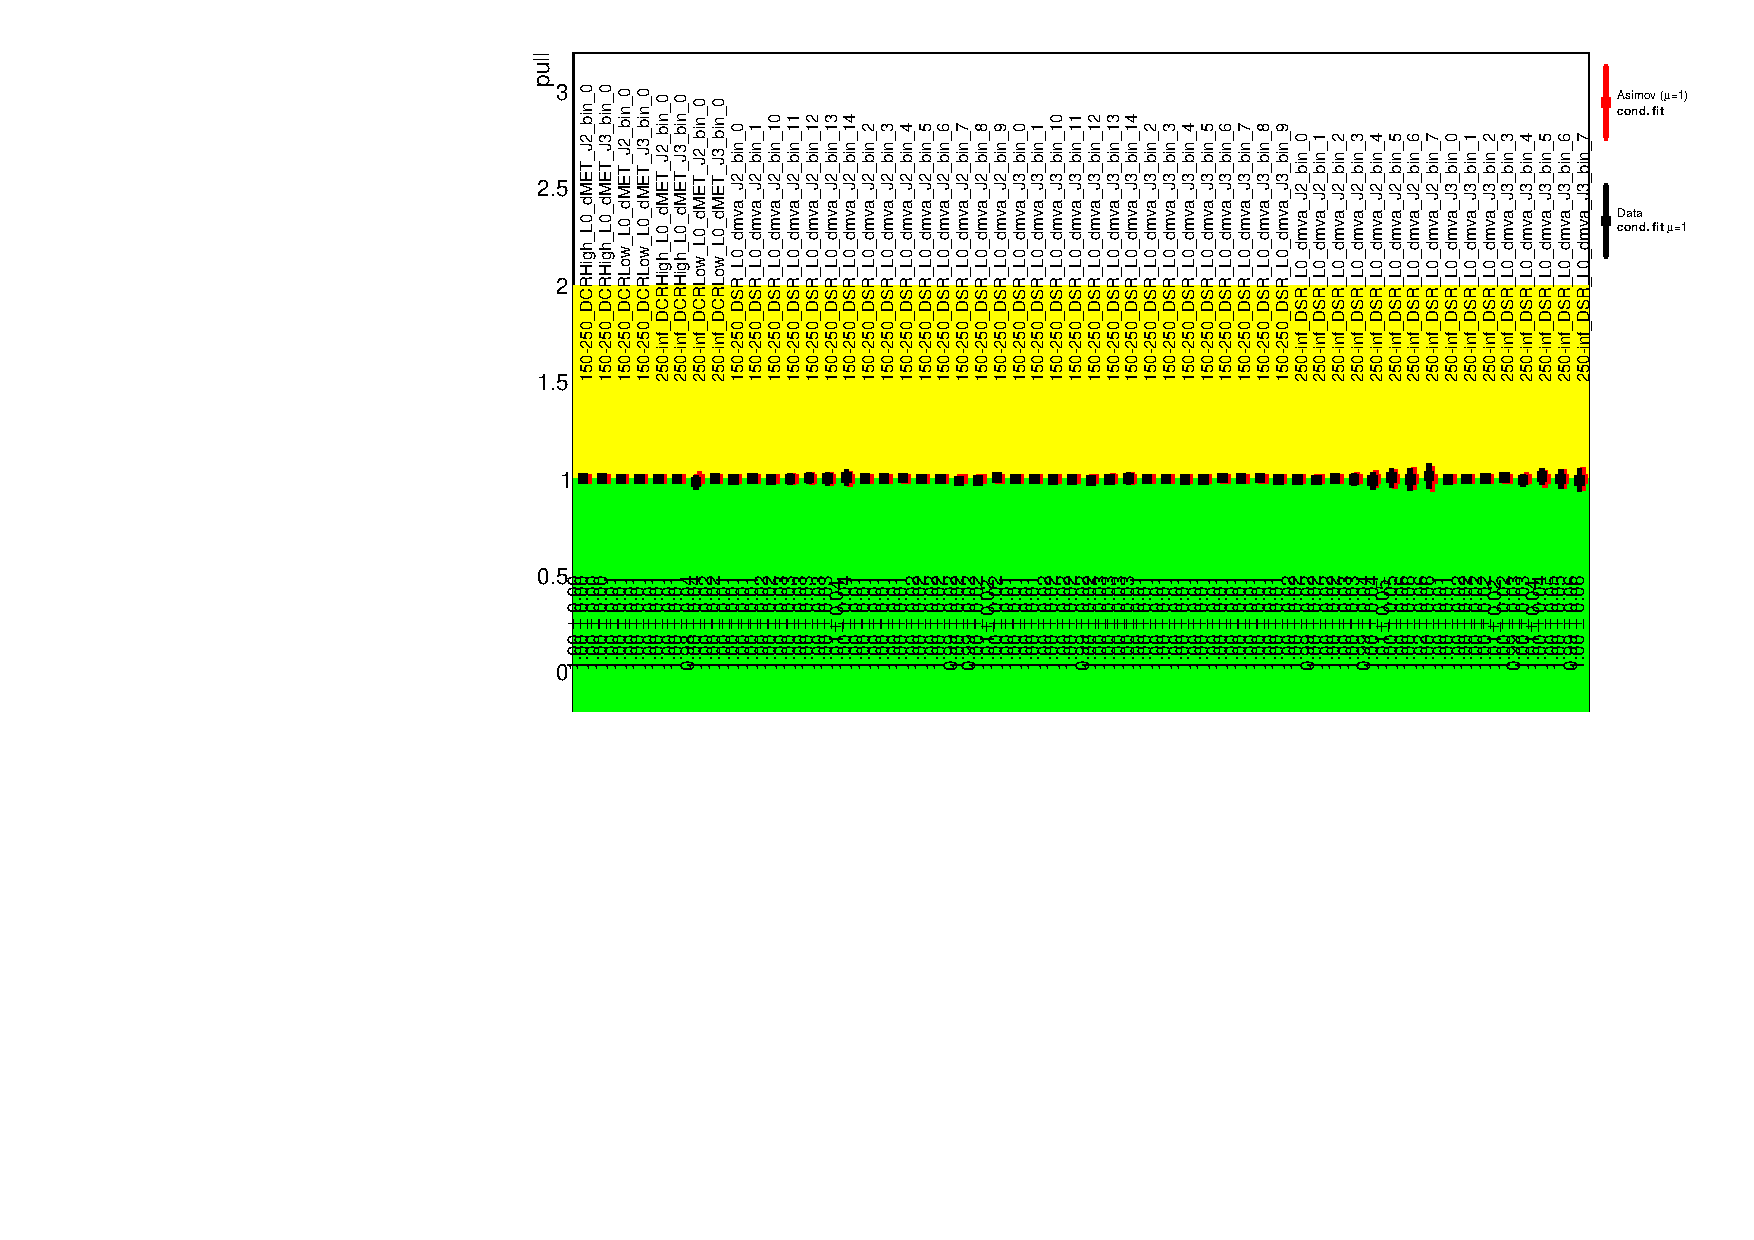
\includegraphics[width=0.49\linewidth]{final_fit_mva/pullComparisons/NP_GammasL0.pdf}
% 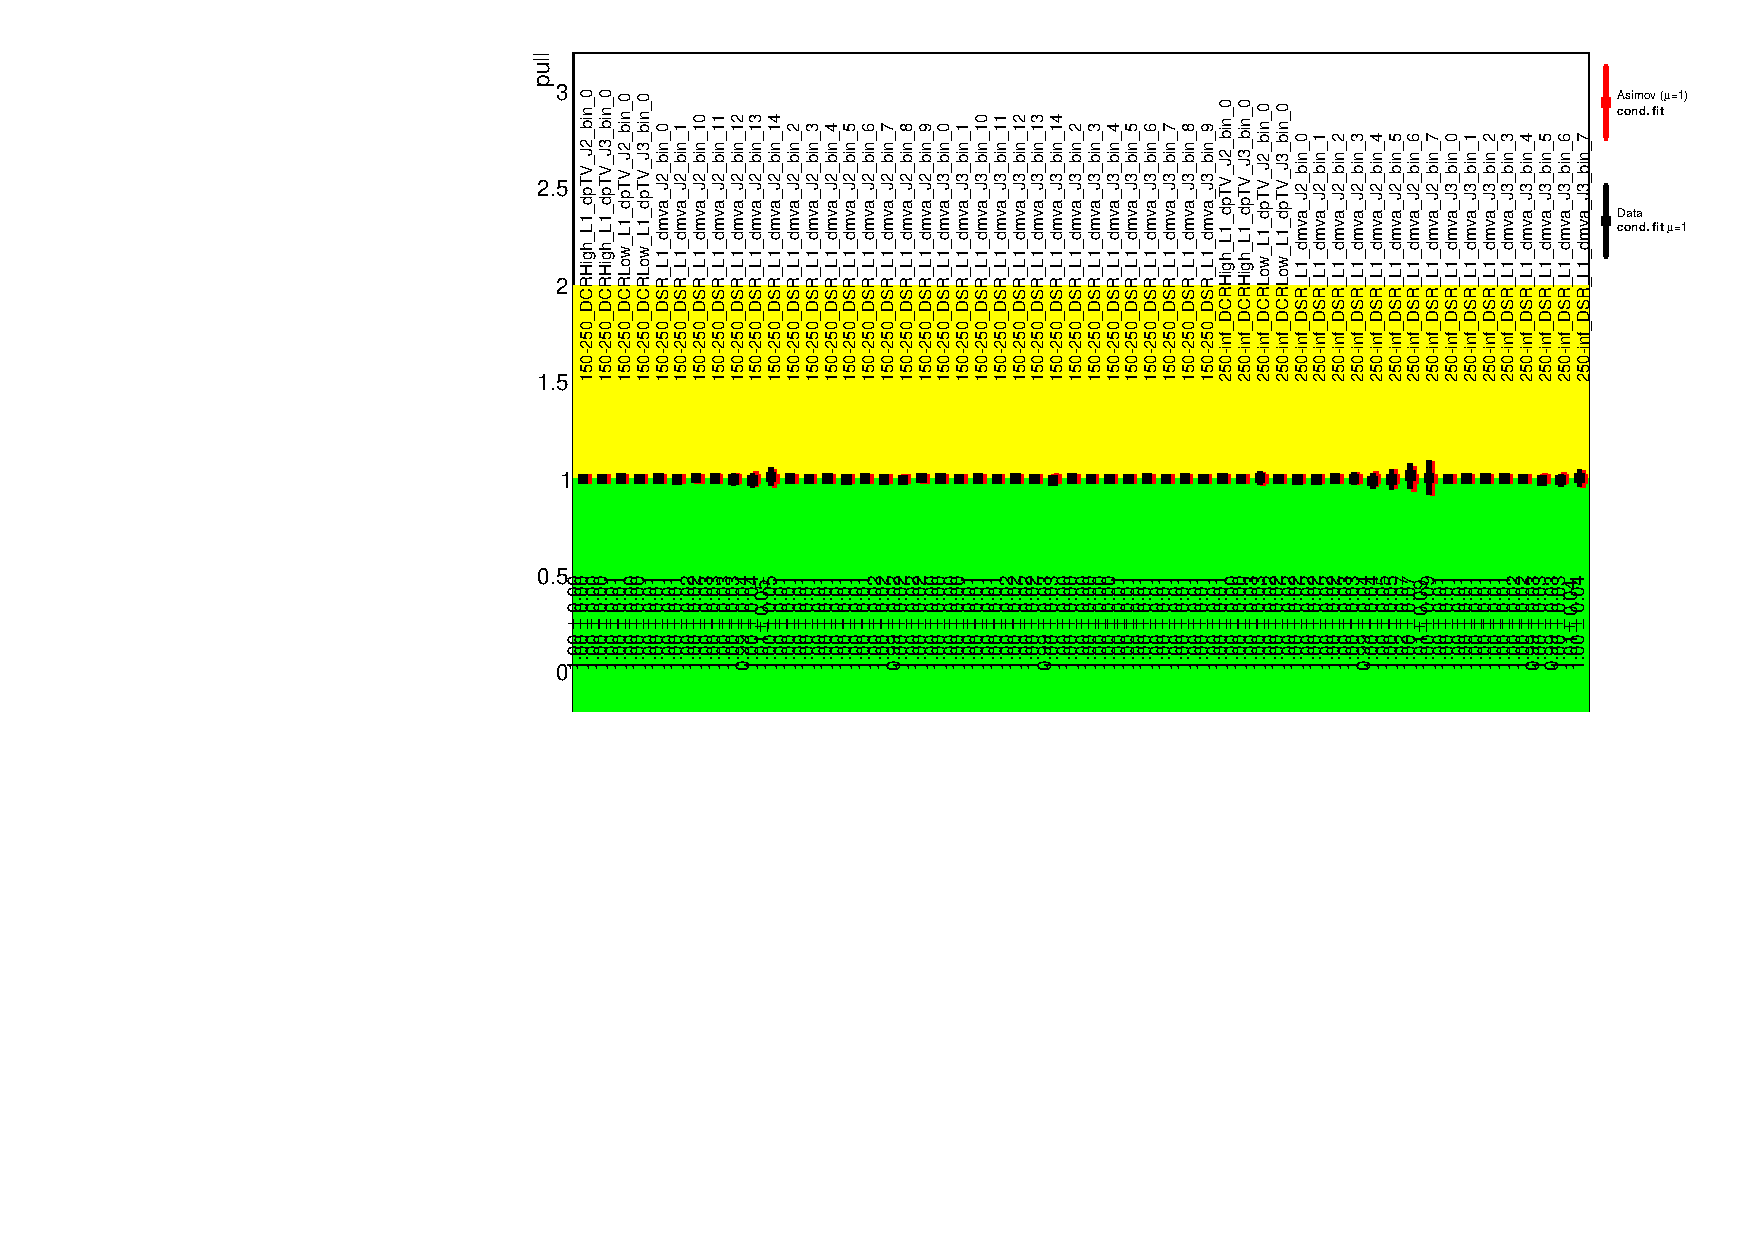
\includegraphics[width=0.49\linewidth]{final_fit_mva/pullComparisons/NP_GammasL1.pdf}
% 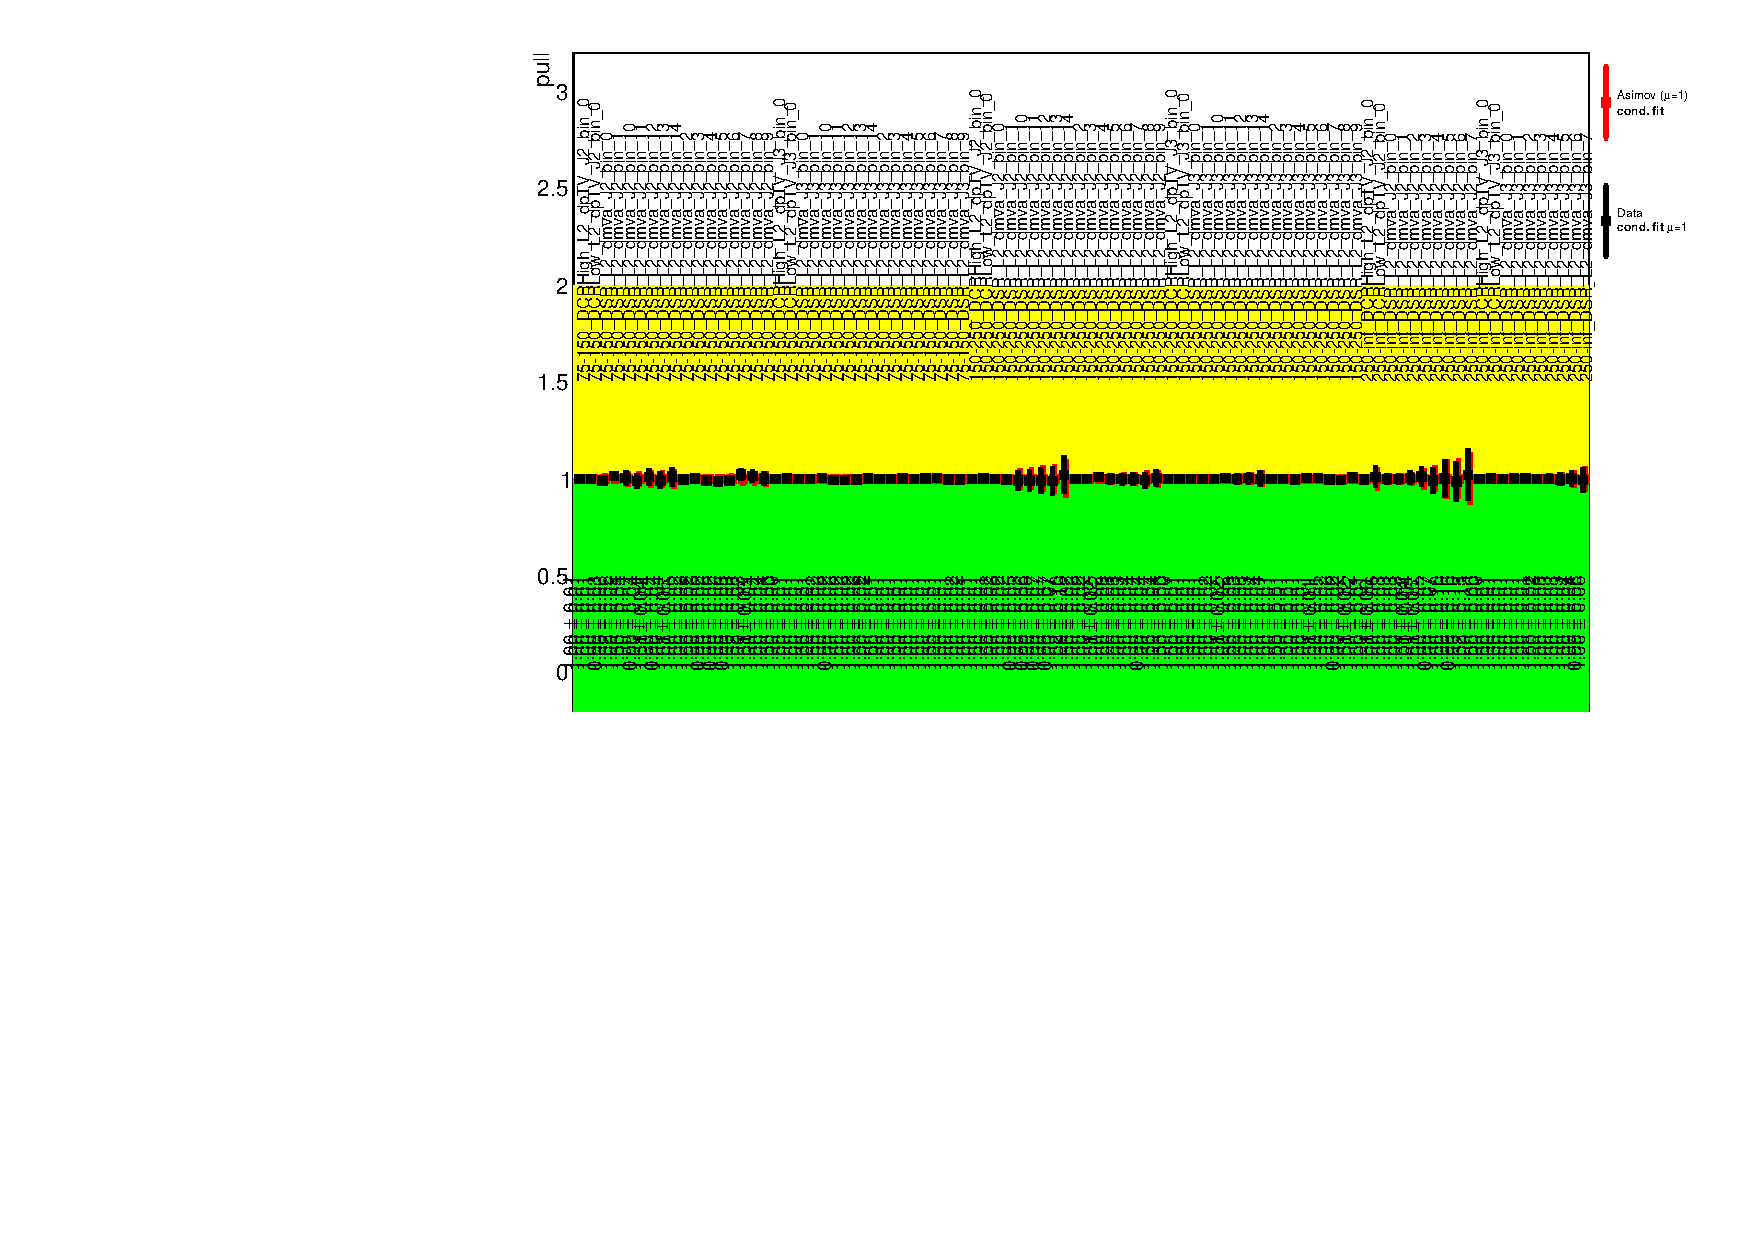
\includegraphics[width=0.49\linewidth]{final_fit_mva/pullComparisons/NP_GammasL2.pdf}
% 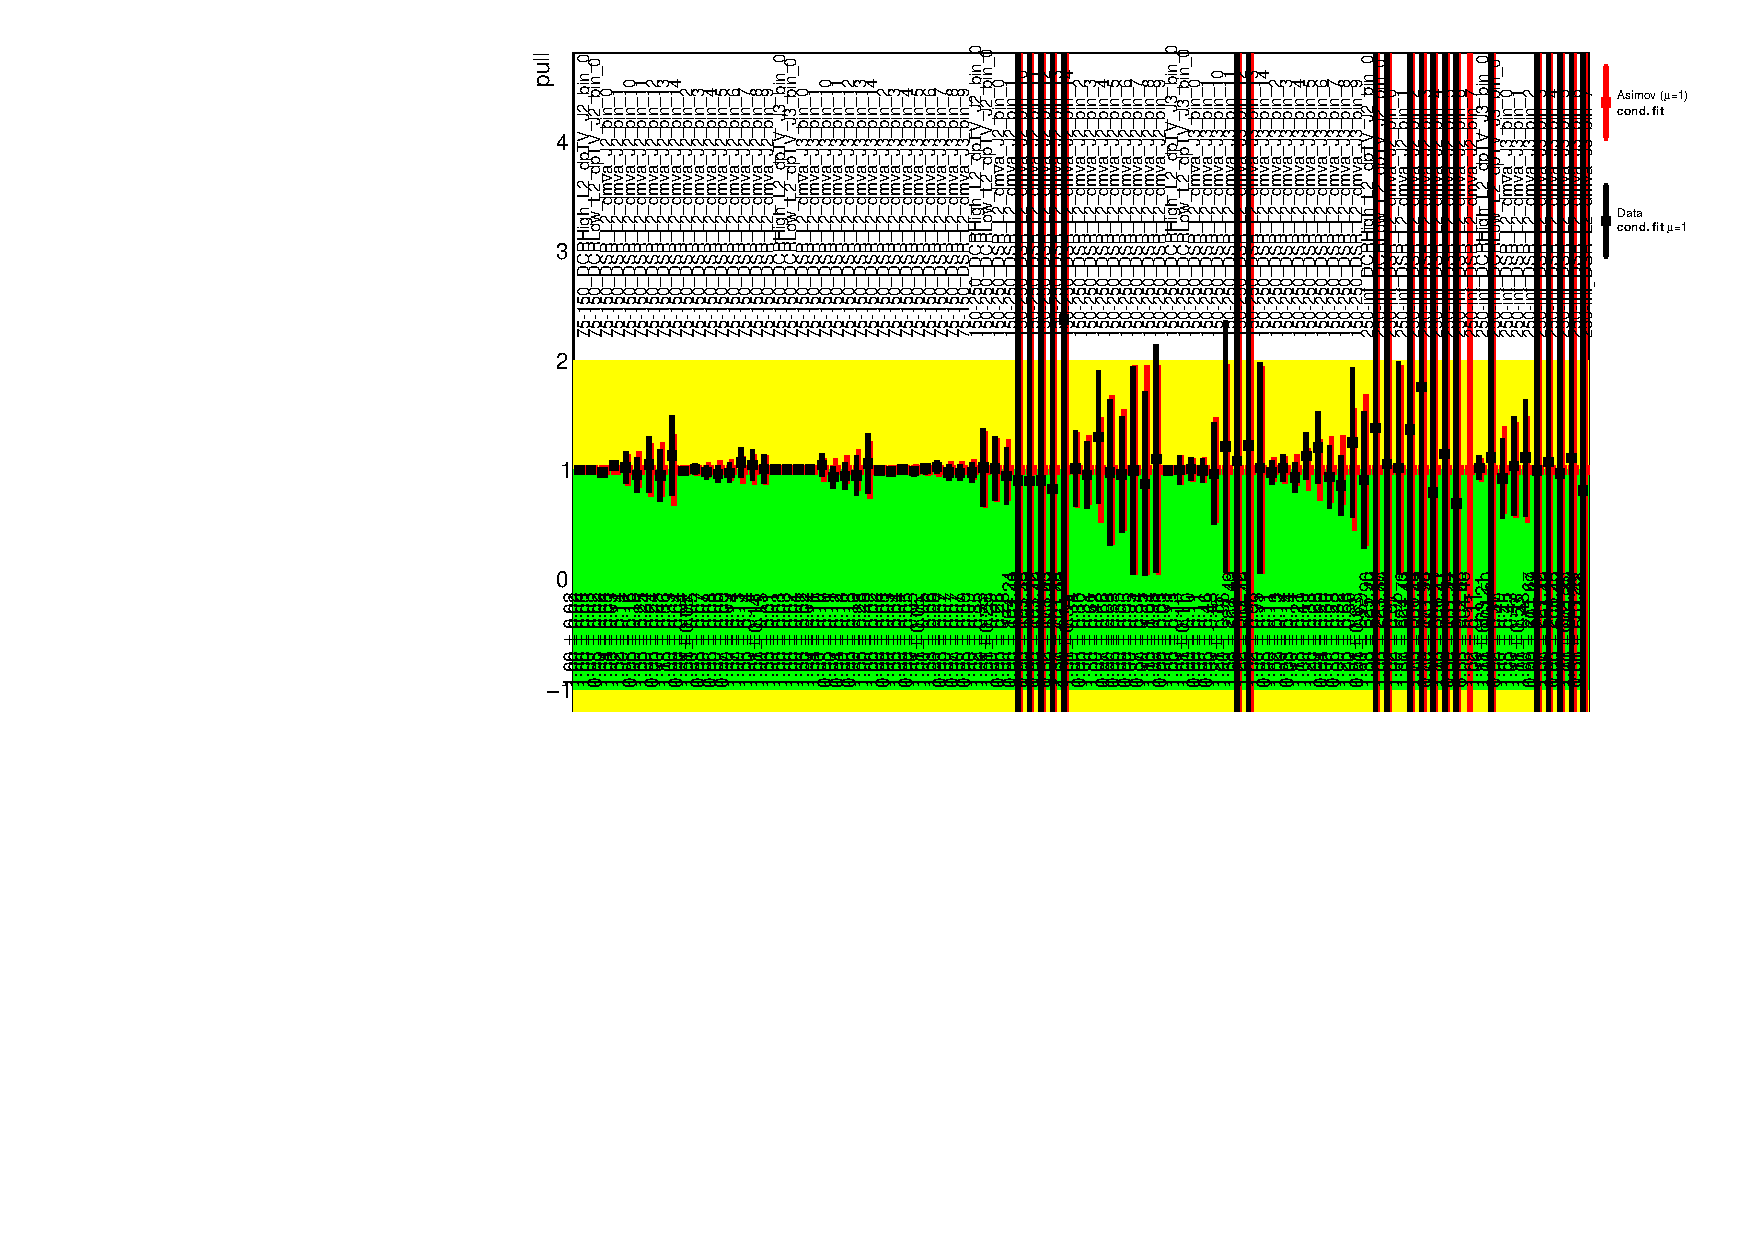
\includegraphics[width=0.49\linewidth]{final_fit_mva/pullComparisons/NP_DDttbar.pdf}
% \caption{caption}
% MC stat. nuisance parameter pulls and the free parameter scale factors
% corresponding to $0$-lepton, $1$-lepton and $2$-lepton as well as the Gamma
% parameter pulls for the data driven top template in the $2$-lepton channel
% corresponding to a conditional combined fit to the Asimov dataset (red) and an
% unconditional combined fit to the \RunTwo data (black)
% \label{fig:nppulls_012L_MVAVH_c} 
% \end{figure}

\subsection{Post-fit Data Versus Predictions}
Describe agreement here.
\begin{figure}
  \centering
  \begin{tabular}{cc}
    % top row
    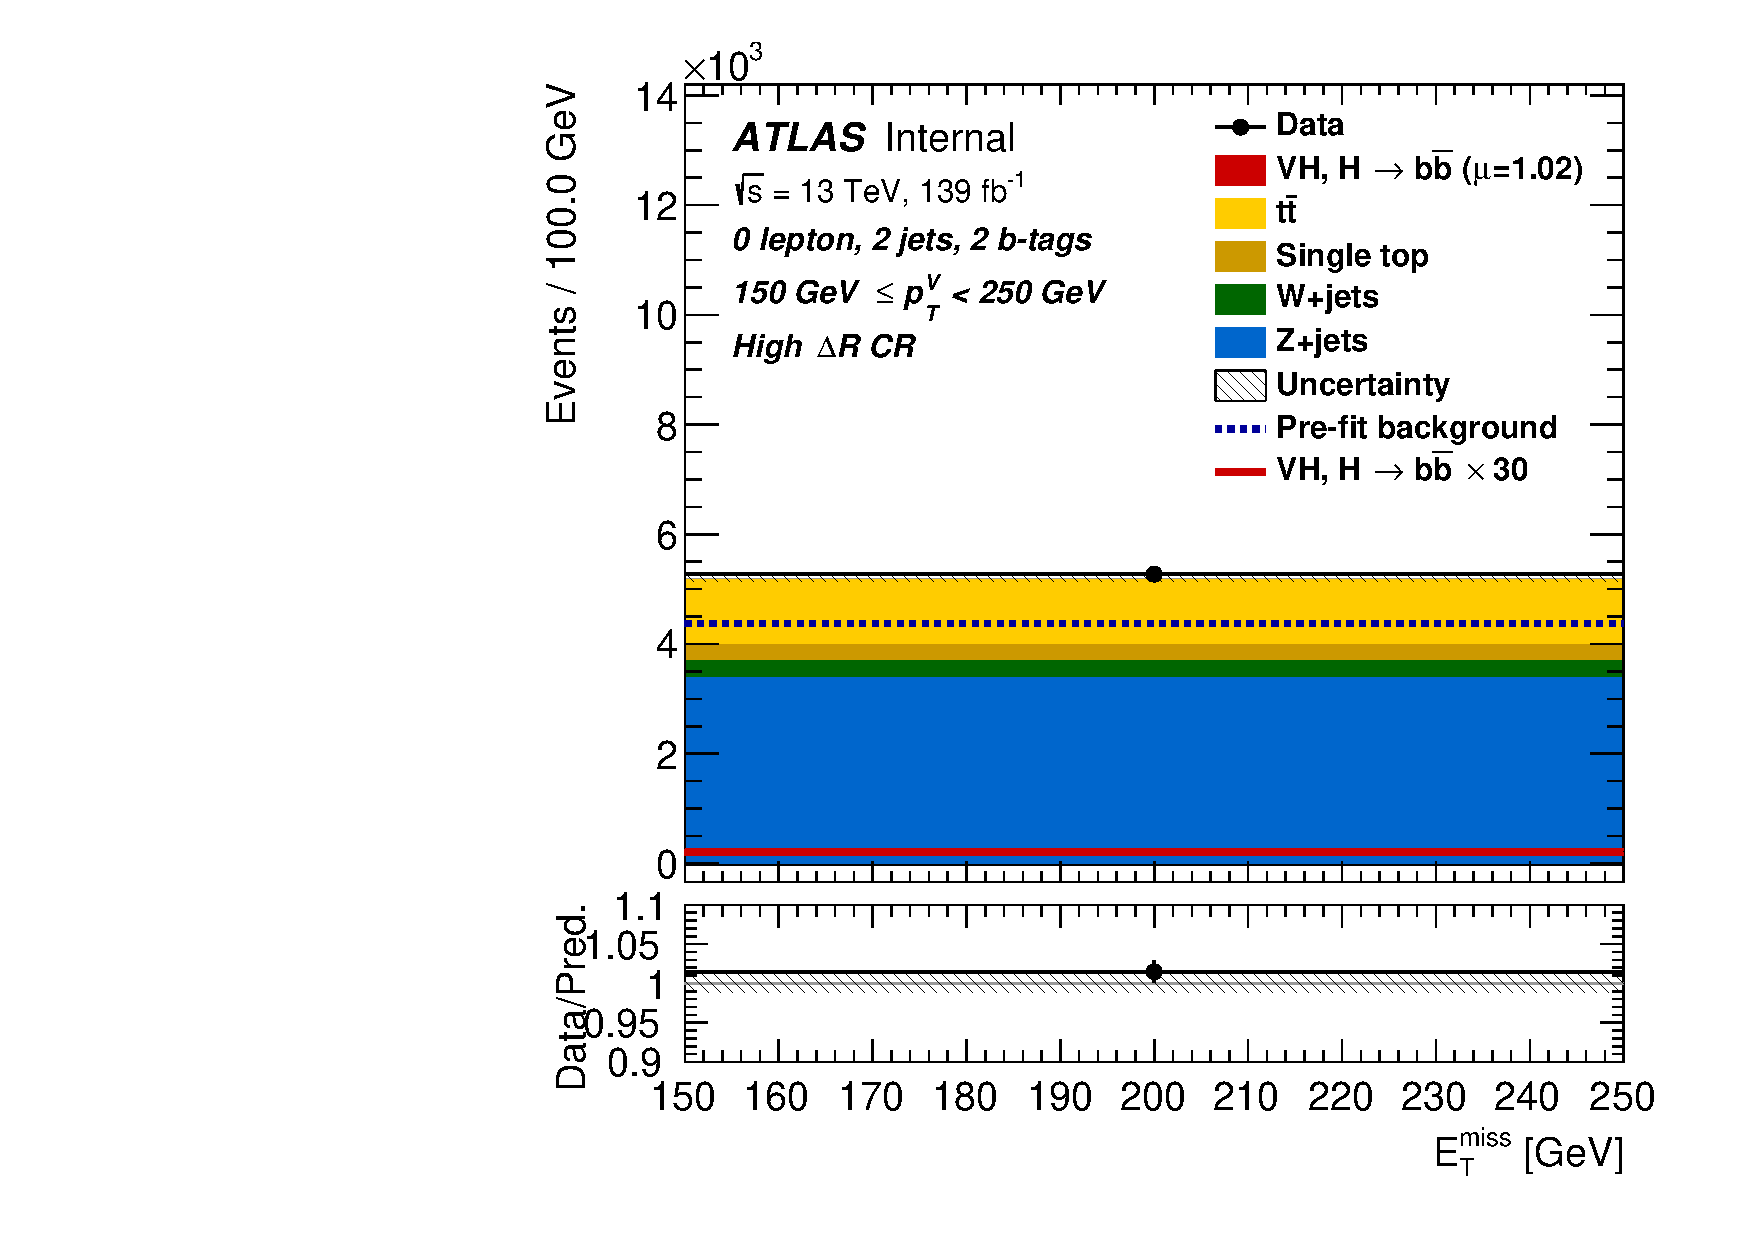
\includegraphics[width=.49\textwidth]{final_fit_mva/postfit/Region_BMax250_BMin150_Y6051_DCRHigh_T2_L0_distMET_J2_GlobalFit_unconditionnal_mu1}%
    & 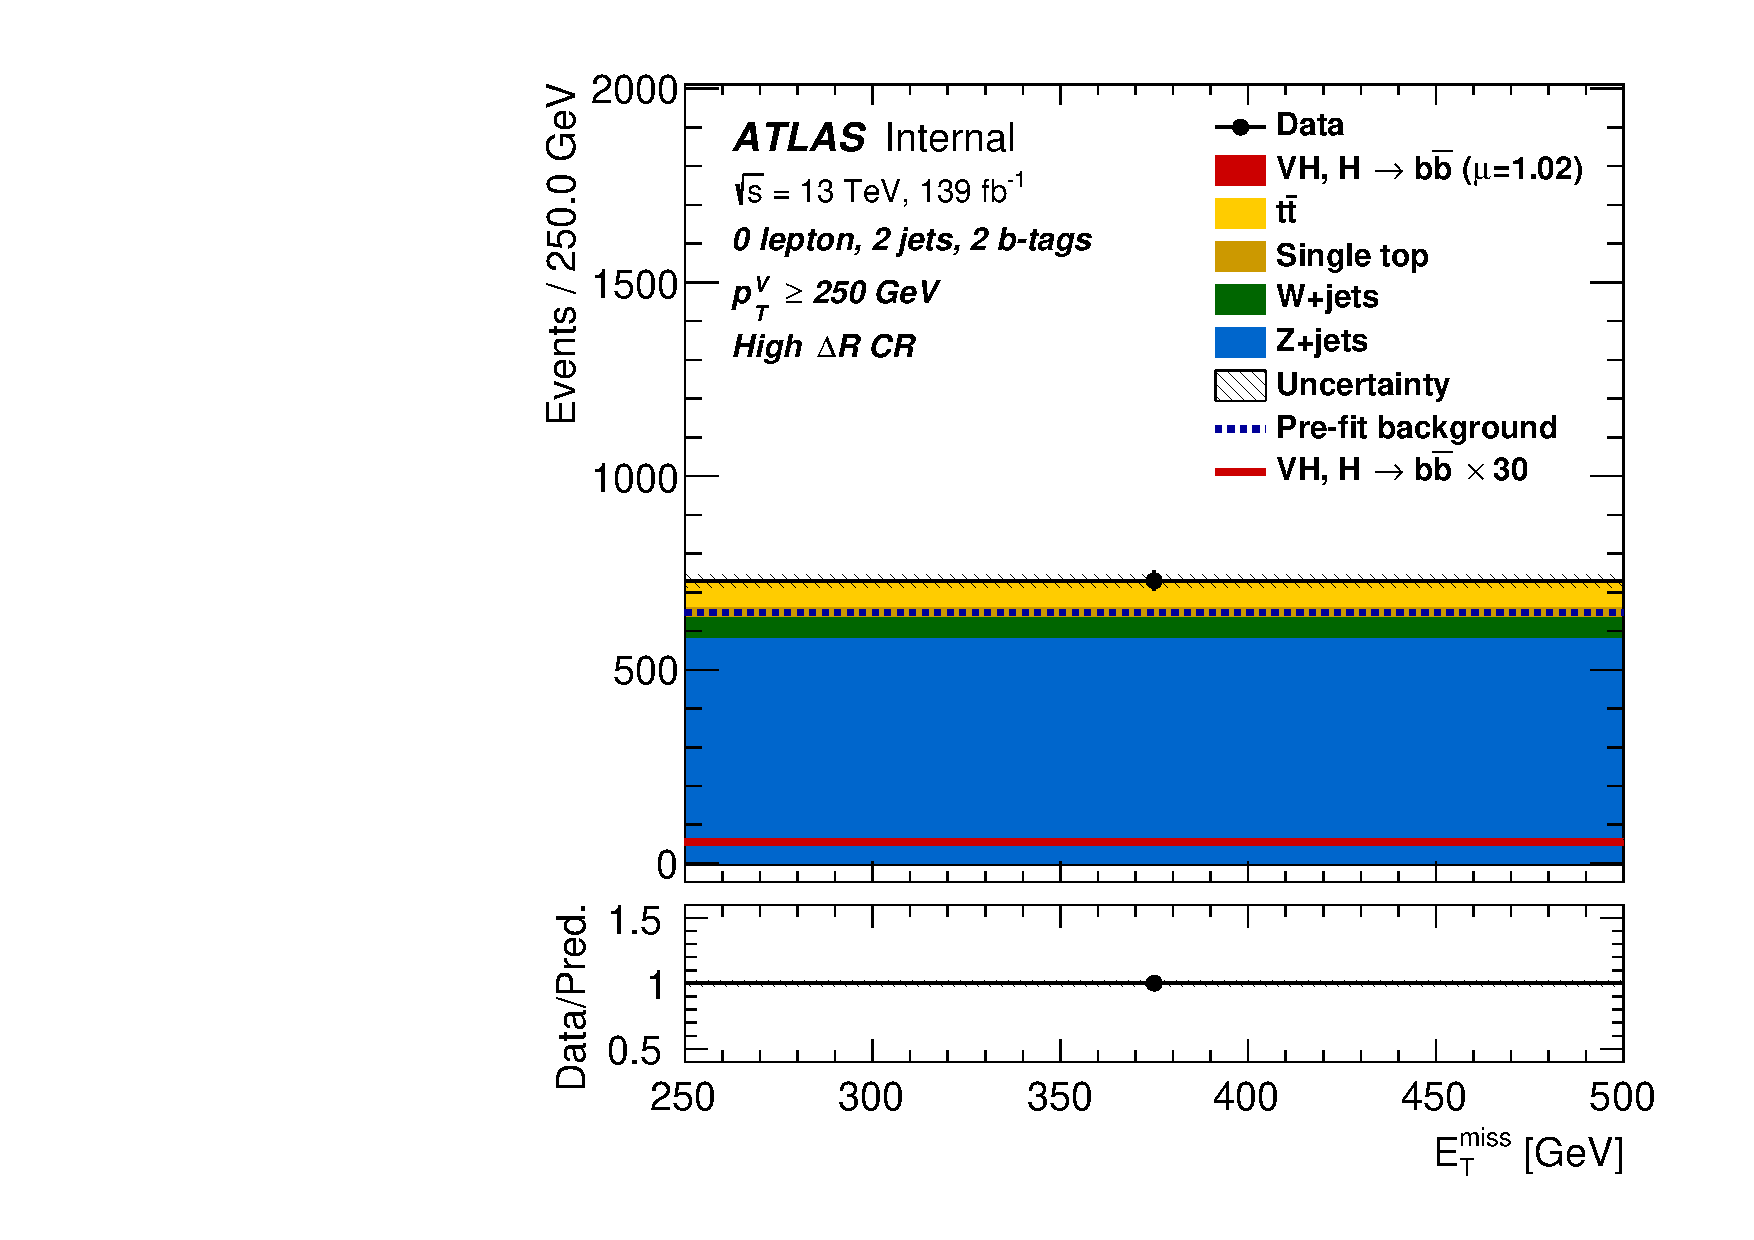
\includegraphics[width=.49\textwidth]{final_fit_mva/postfit/Region_BMin250_Y6051_DCRHigh_T2_L0_distMET_J2_GlobalFit_unconditionnal_mu1} \\

    % middle row
    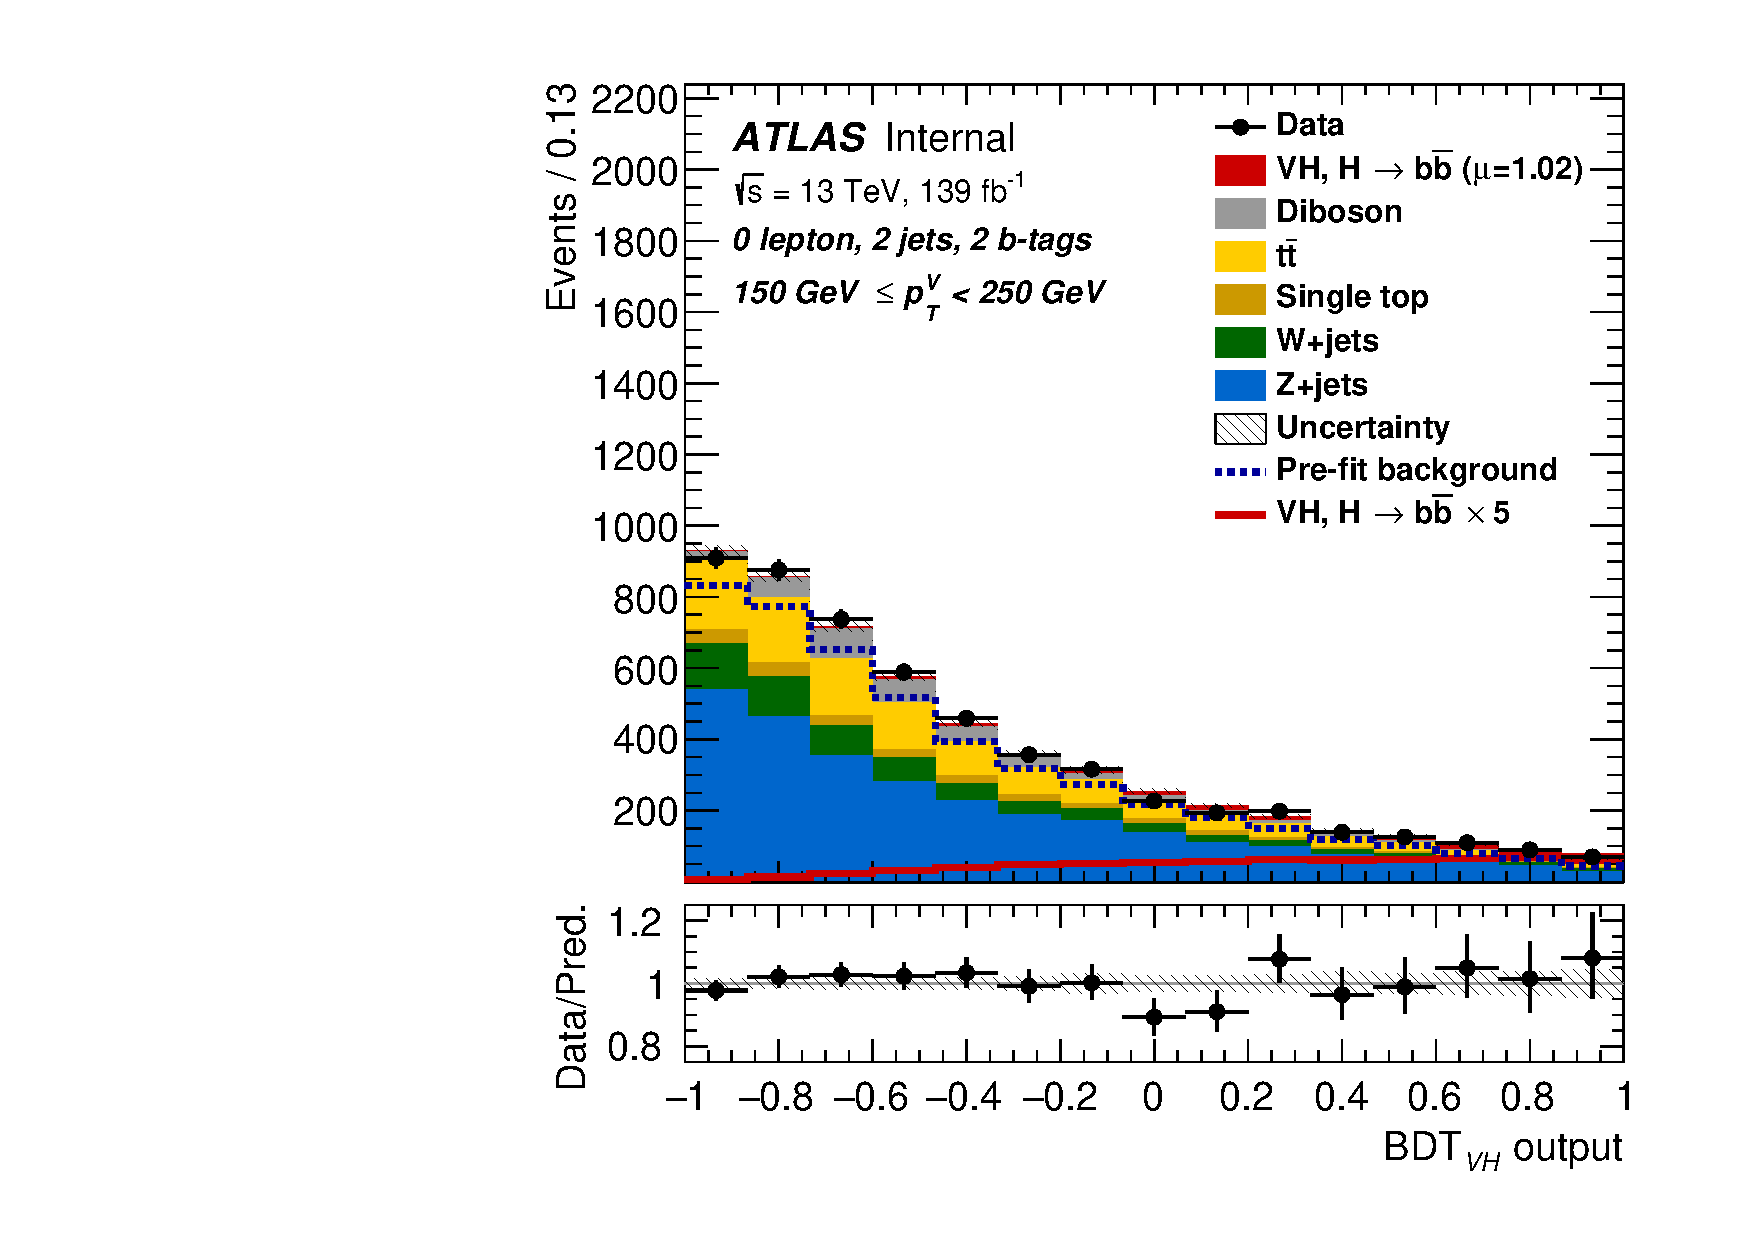
\includegraphics[width=.49\textwidth]{final_fit_mva/postfit/Region_BMax250_BMin150_Y6051_DSR_T2_L0_distmva_J2_GlobalFit_unconditionnal_mu1}%
    & 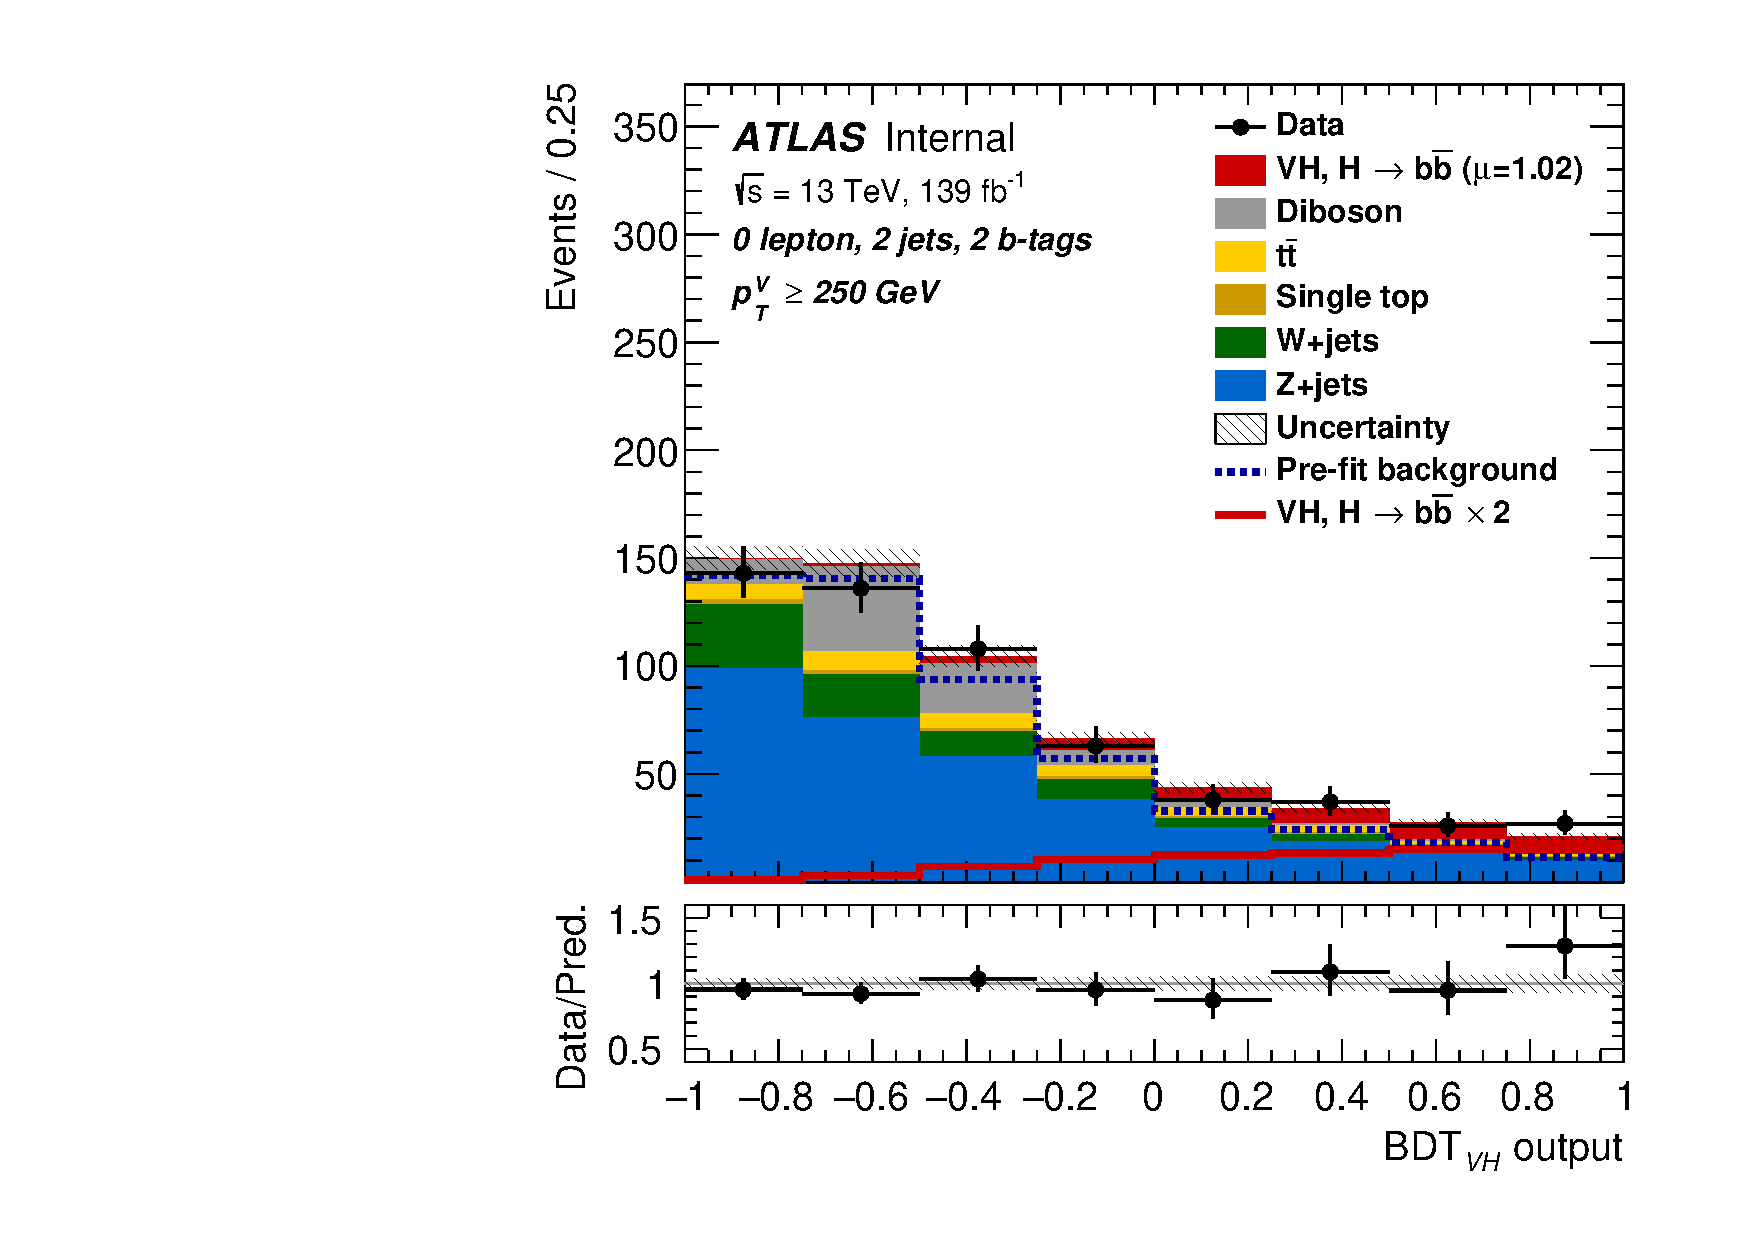
\includegraphics[width=.49\textwidth]{final_fit_mva/postfit/Region_BMin250_Y6051_DSR_T2_L0_distmva_J2_GlobalFit_unconditionnal_mu1} \\

    % bottom row
    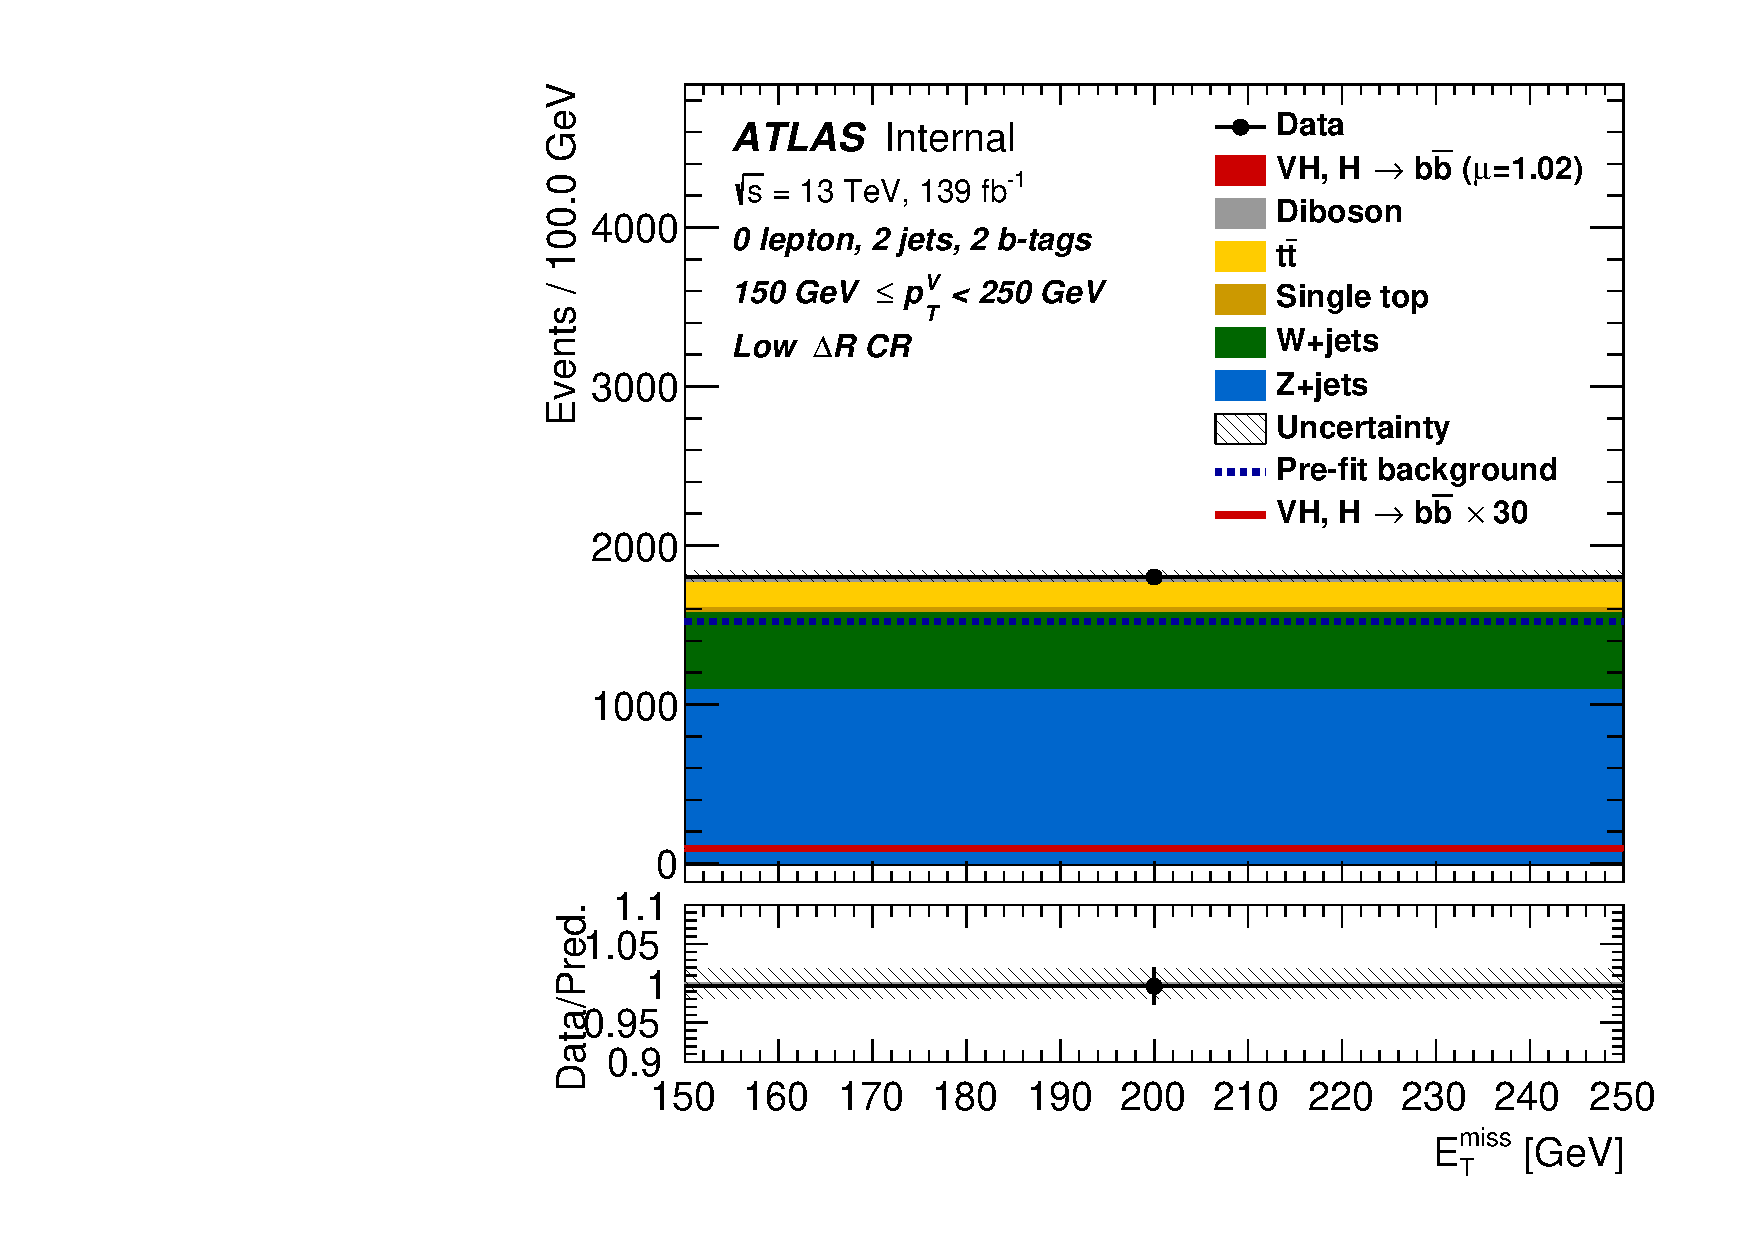
\includegraphics[width=.49\textwidth]{final_fit_mva/postfit/Region_BMax250_BMin150_Y6051_DCRLow_T2_L0_distMET_J2_GlobalFit_unconditionnal_mu1}%
    & 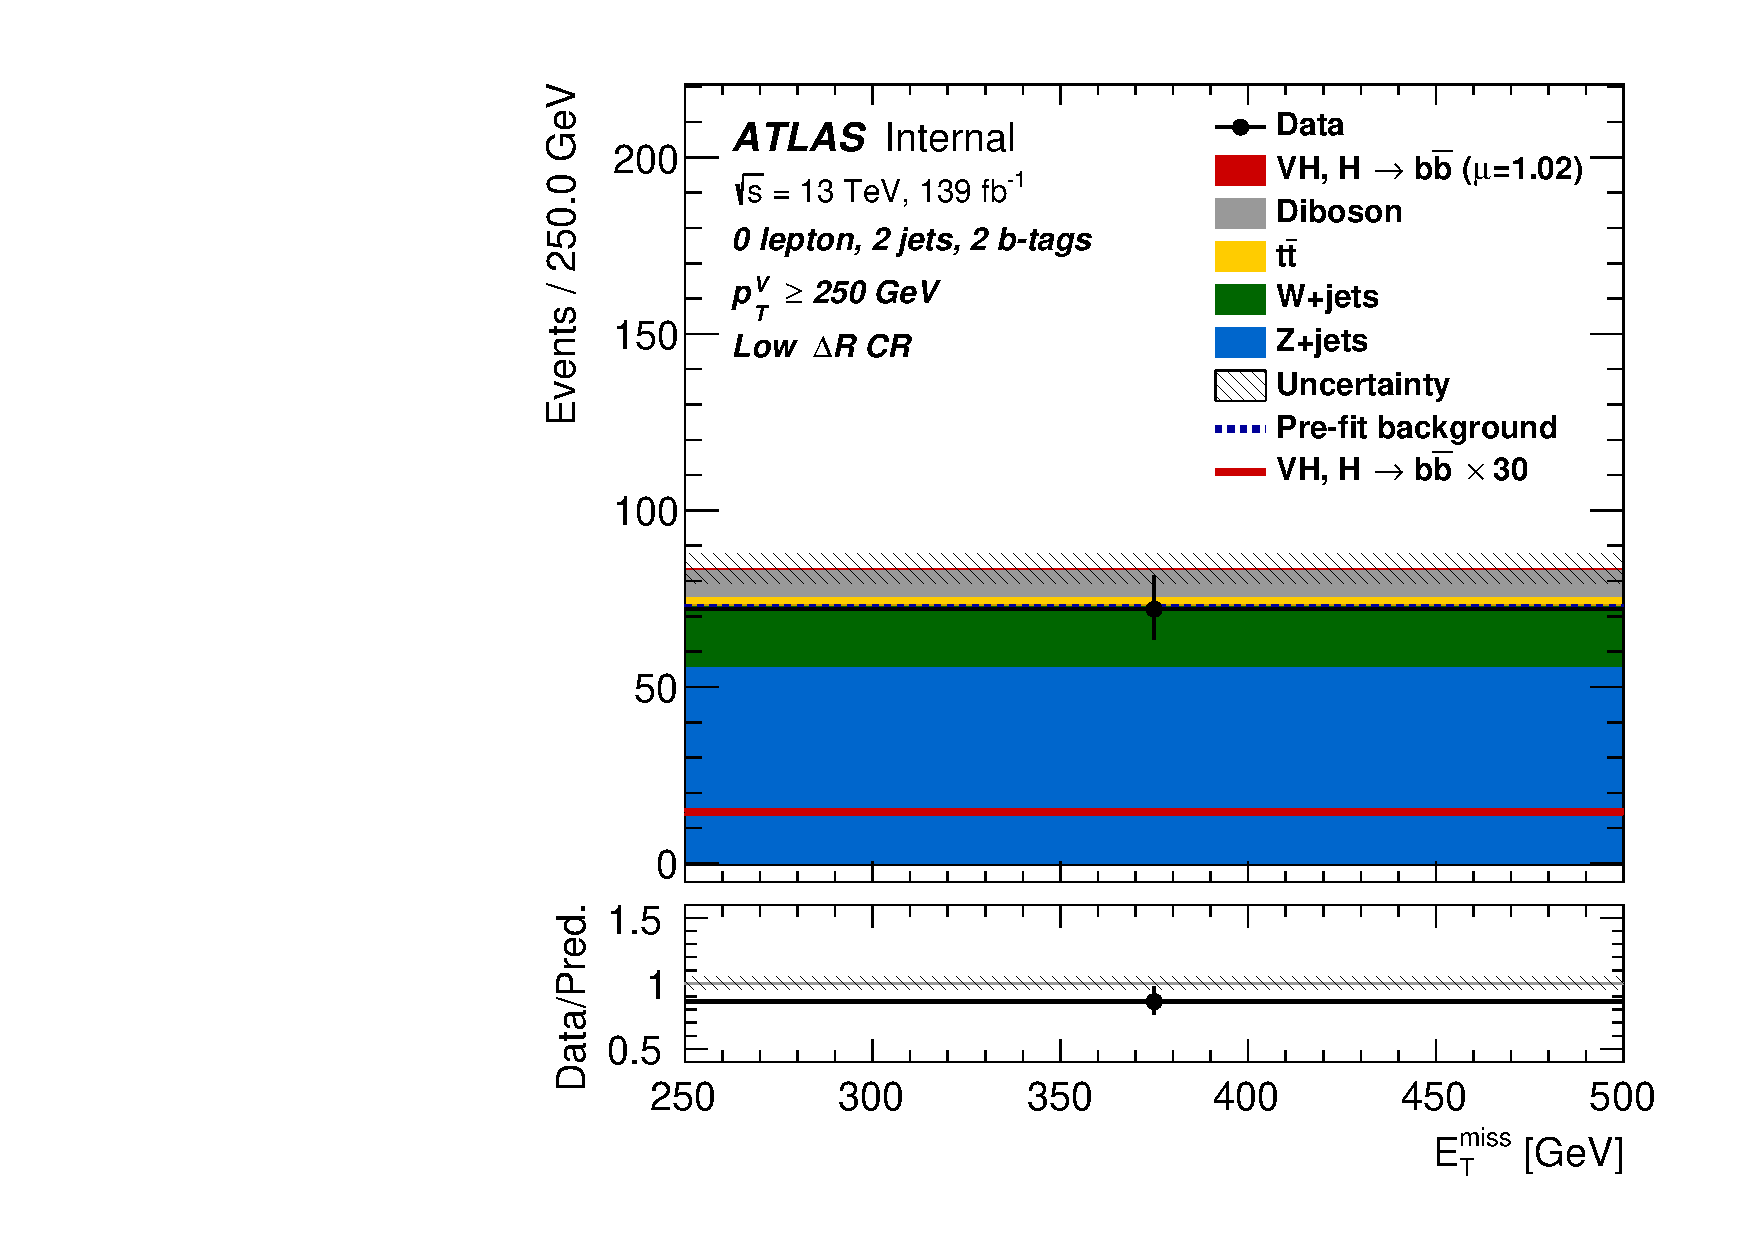
\includegraphics[width=.49\textwidth]{final_fit_mva/postfit/Region_BMin250_Y6051_DCRLow_T2_L0_distMET_J2_GlobalFit_unconditionnal_mu1} \\
  \end{tabular}
  \caption{Post-fit distributions in the 0--lepton 2--jet channel.}
  \label{fig:0lep2jet-postfit}
\end{figure}
\begin{figure}
  \centering
  \begin{tabular}{cc}
    % top row
    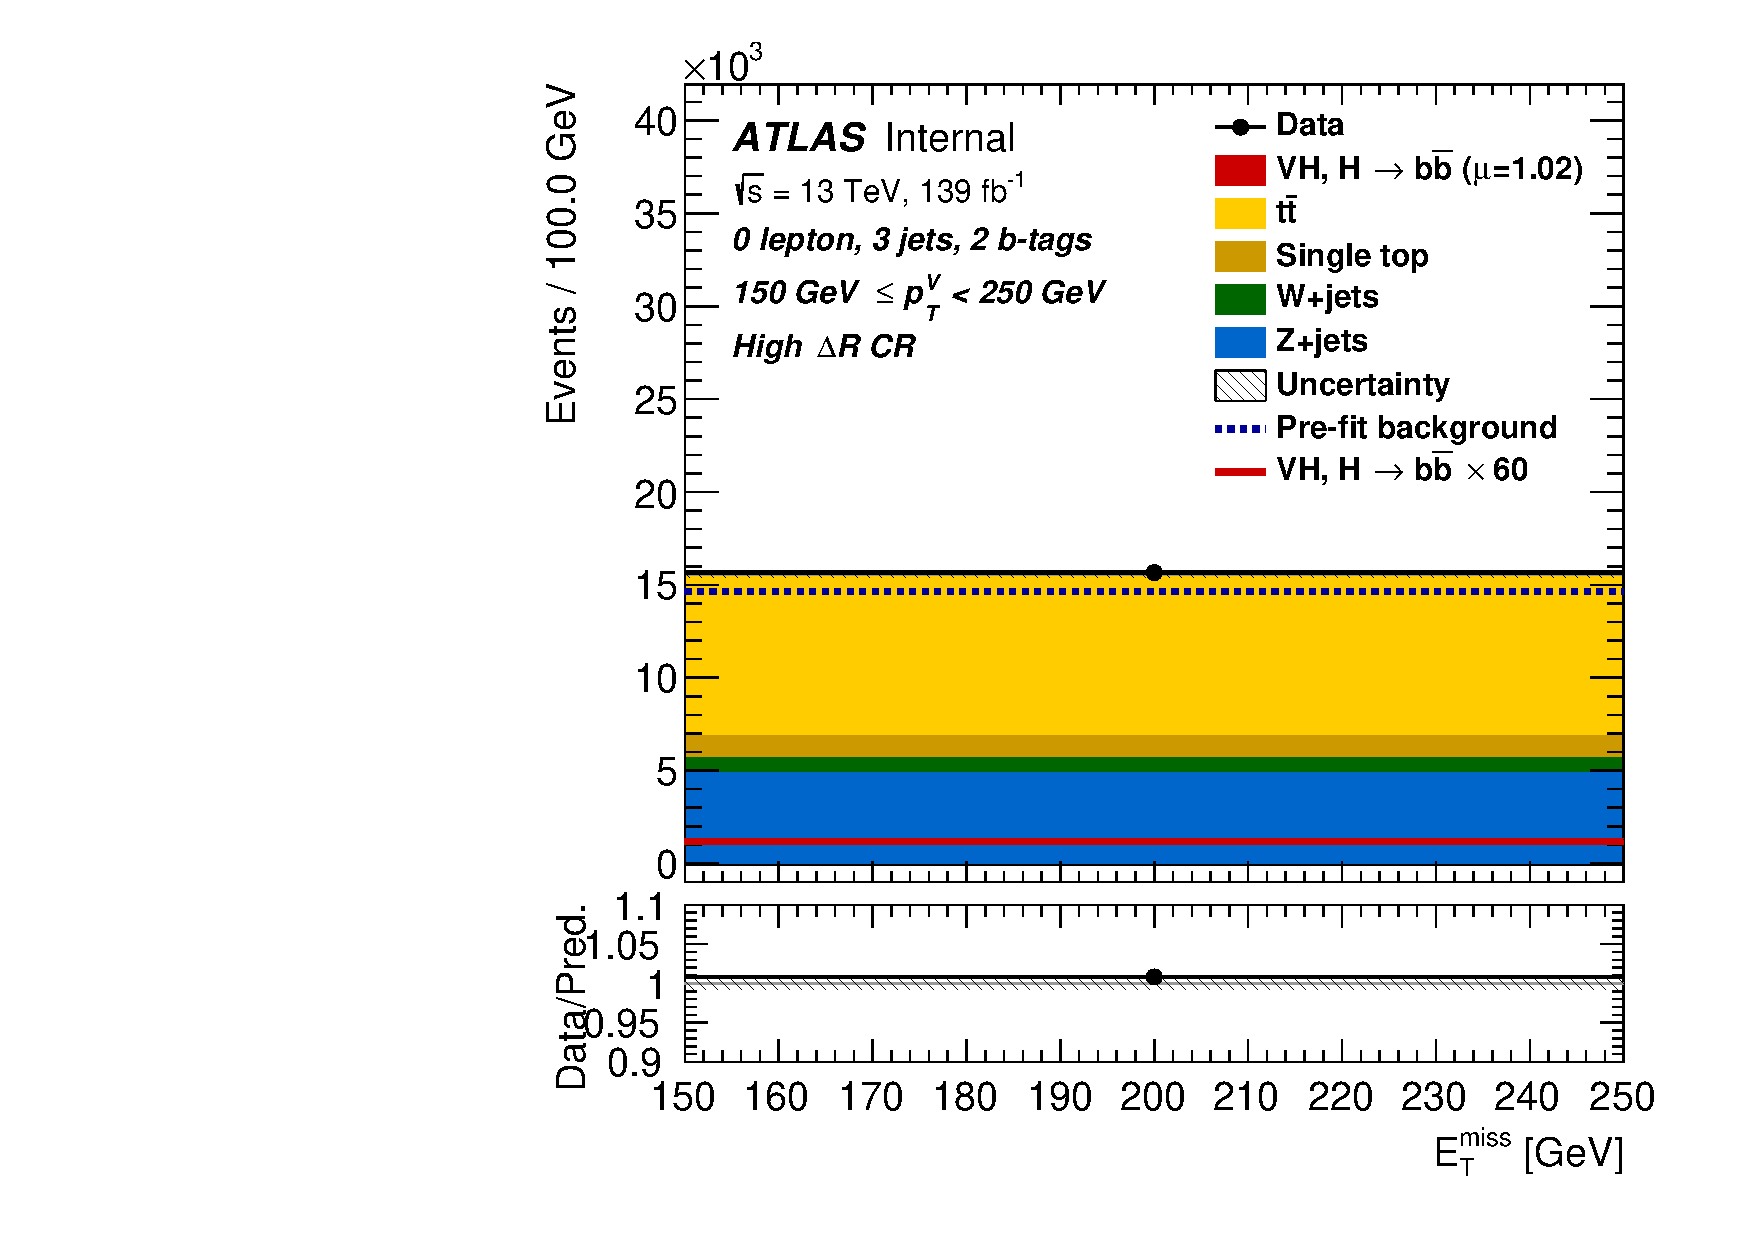
\includegraphics[width=.3\textwidth]{final_fit_mva/postfit/Region_BMax250_BMin150_Y6051_DCRHigh_T2_L0_distMET_J3_GlobalFit_unconditionnal_mu1}%
    & 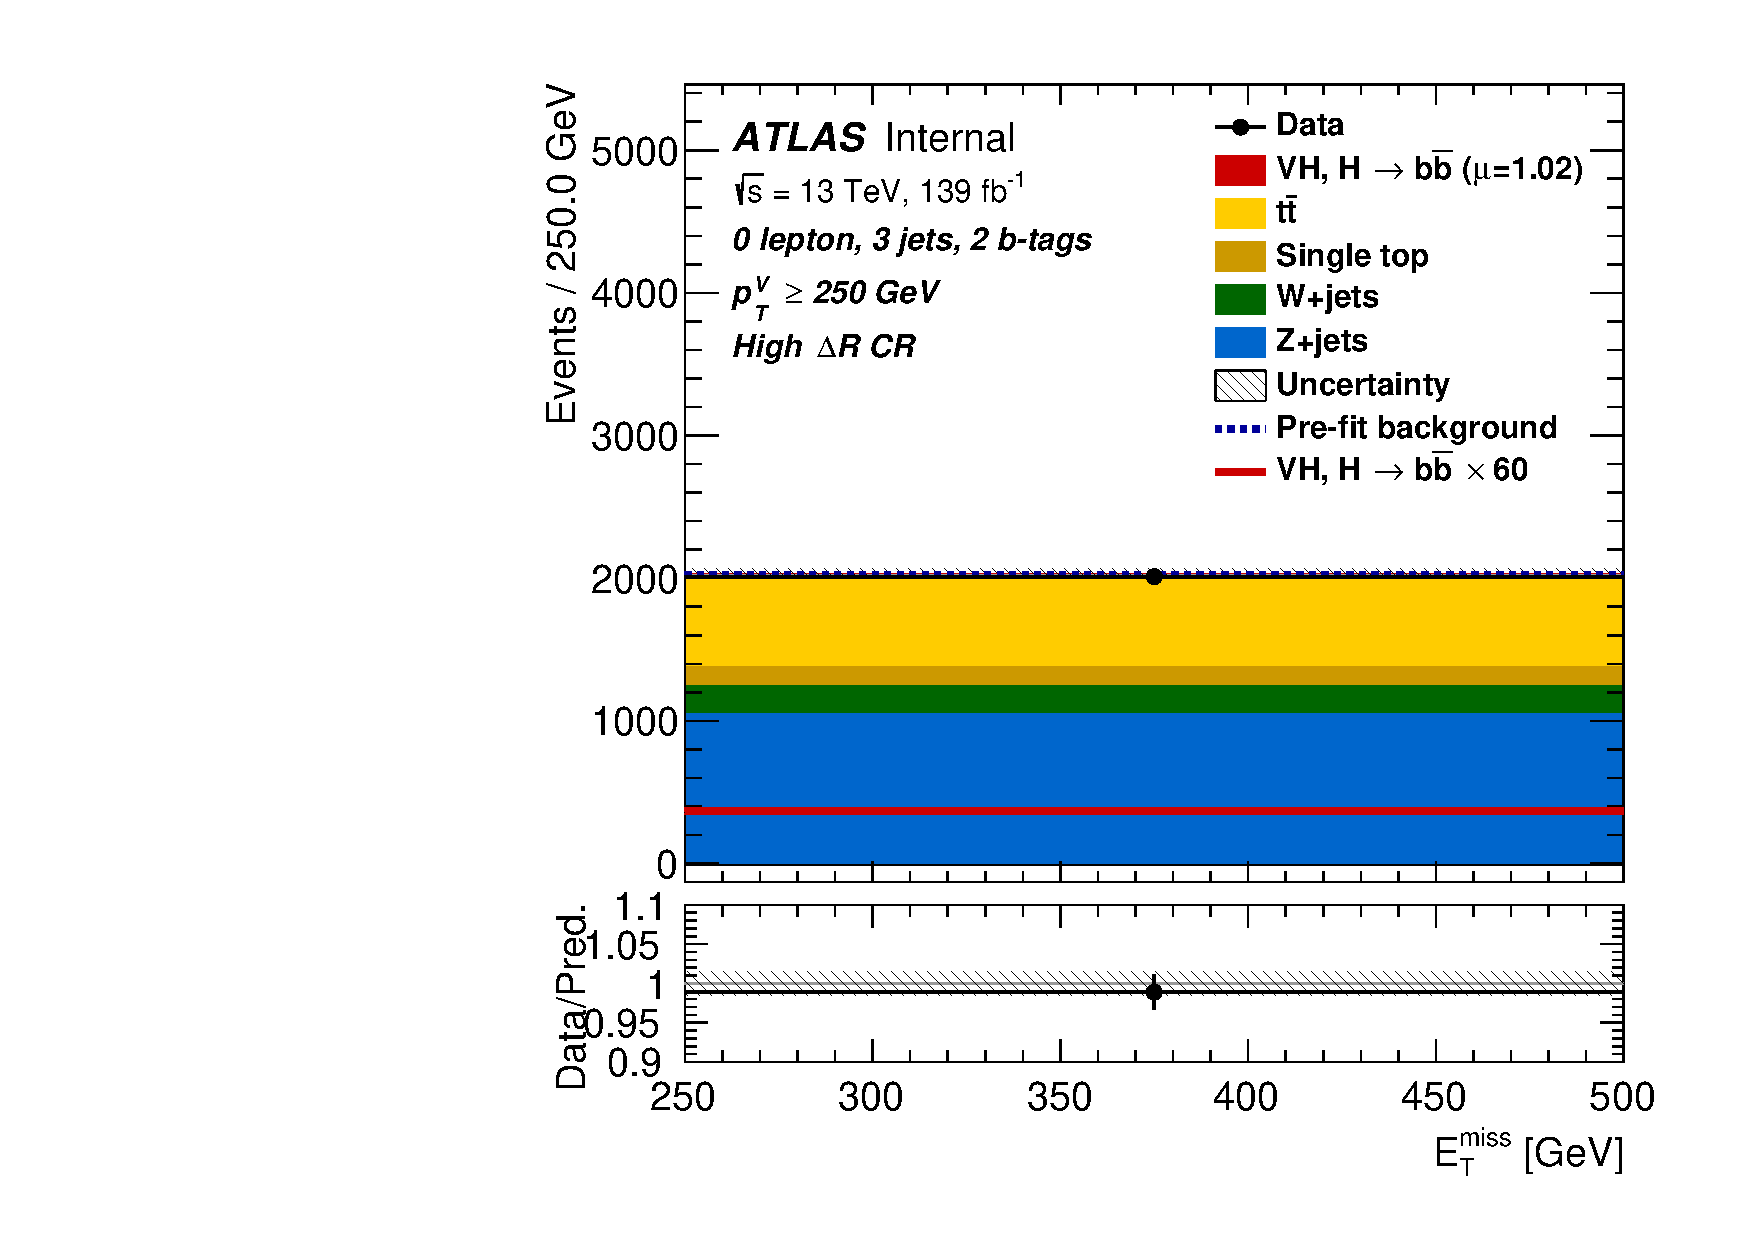
\includegraphics[width=.3\textwidth]{final_fit_mva/postfit/Region_BMin250_Y6051_DCRHigh_T2_L0_distMET_J3_GlobalFit_unconditionnal_mu1} \\

    % middle row
    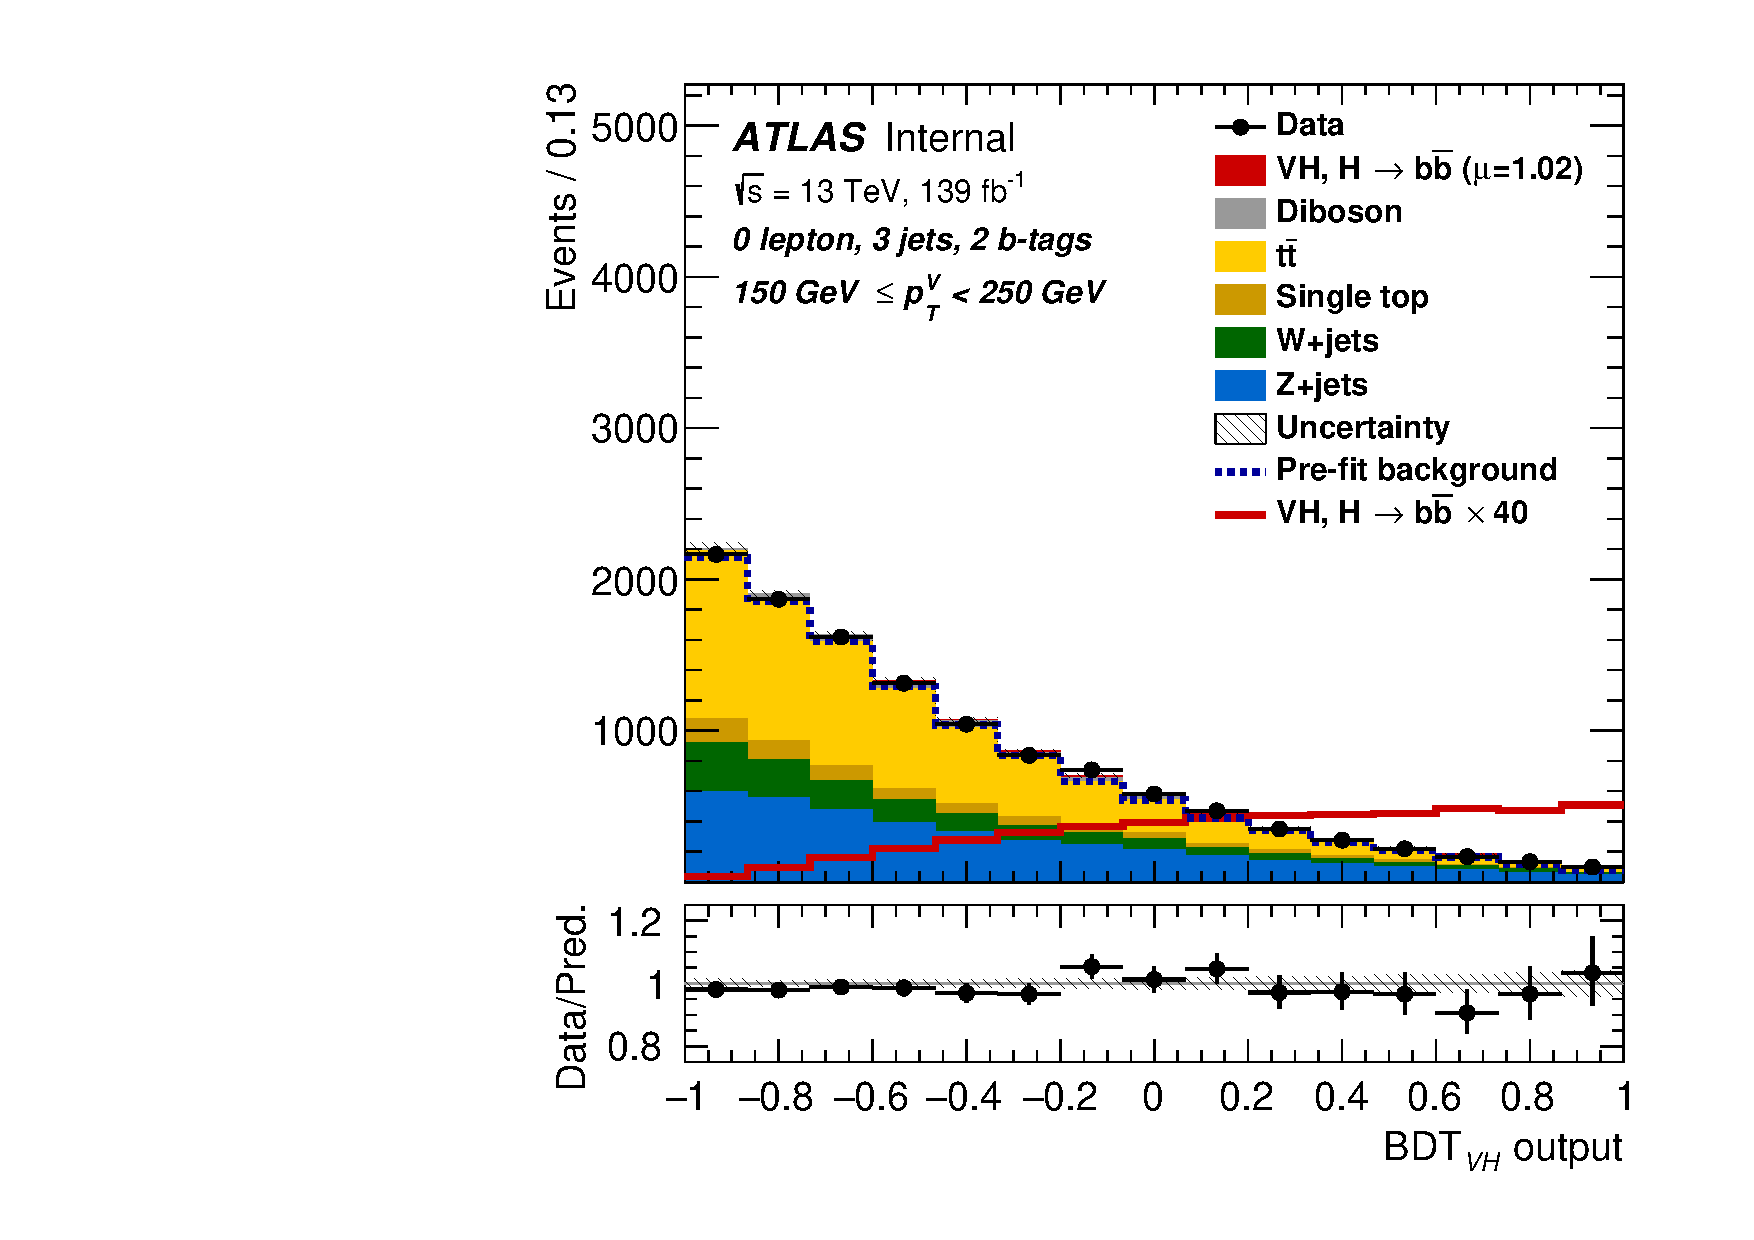
\includegraphics[width=.3\textwidth]{final_fit_mva/postfit/Region_BMax250_BMin150_Y6051_DSR_T2_L0_distmva_J3_GlobalFit_unconditionnal_mu1}%
    & 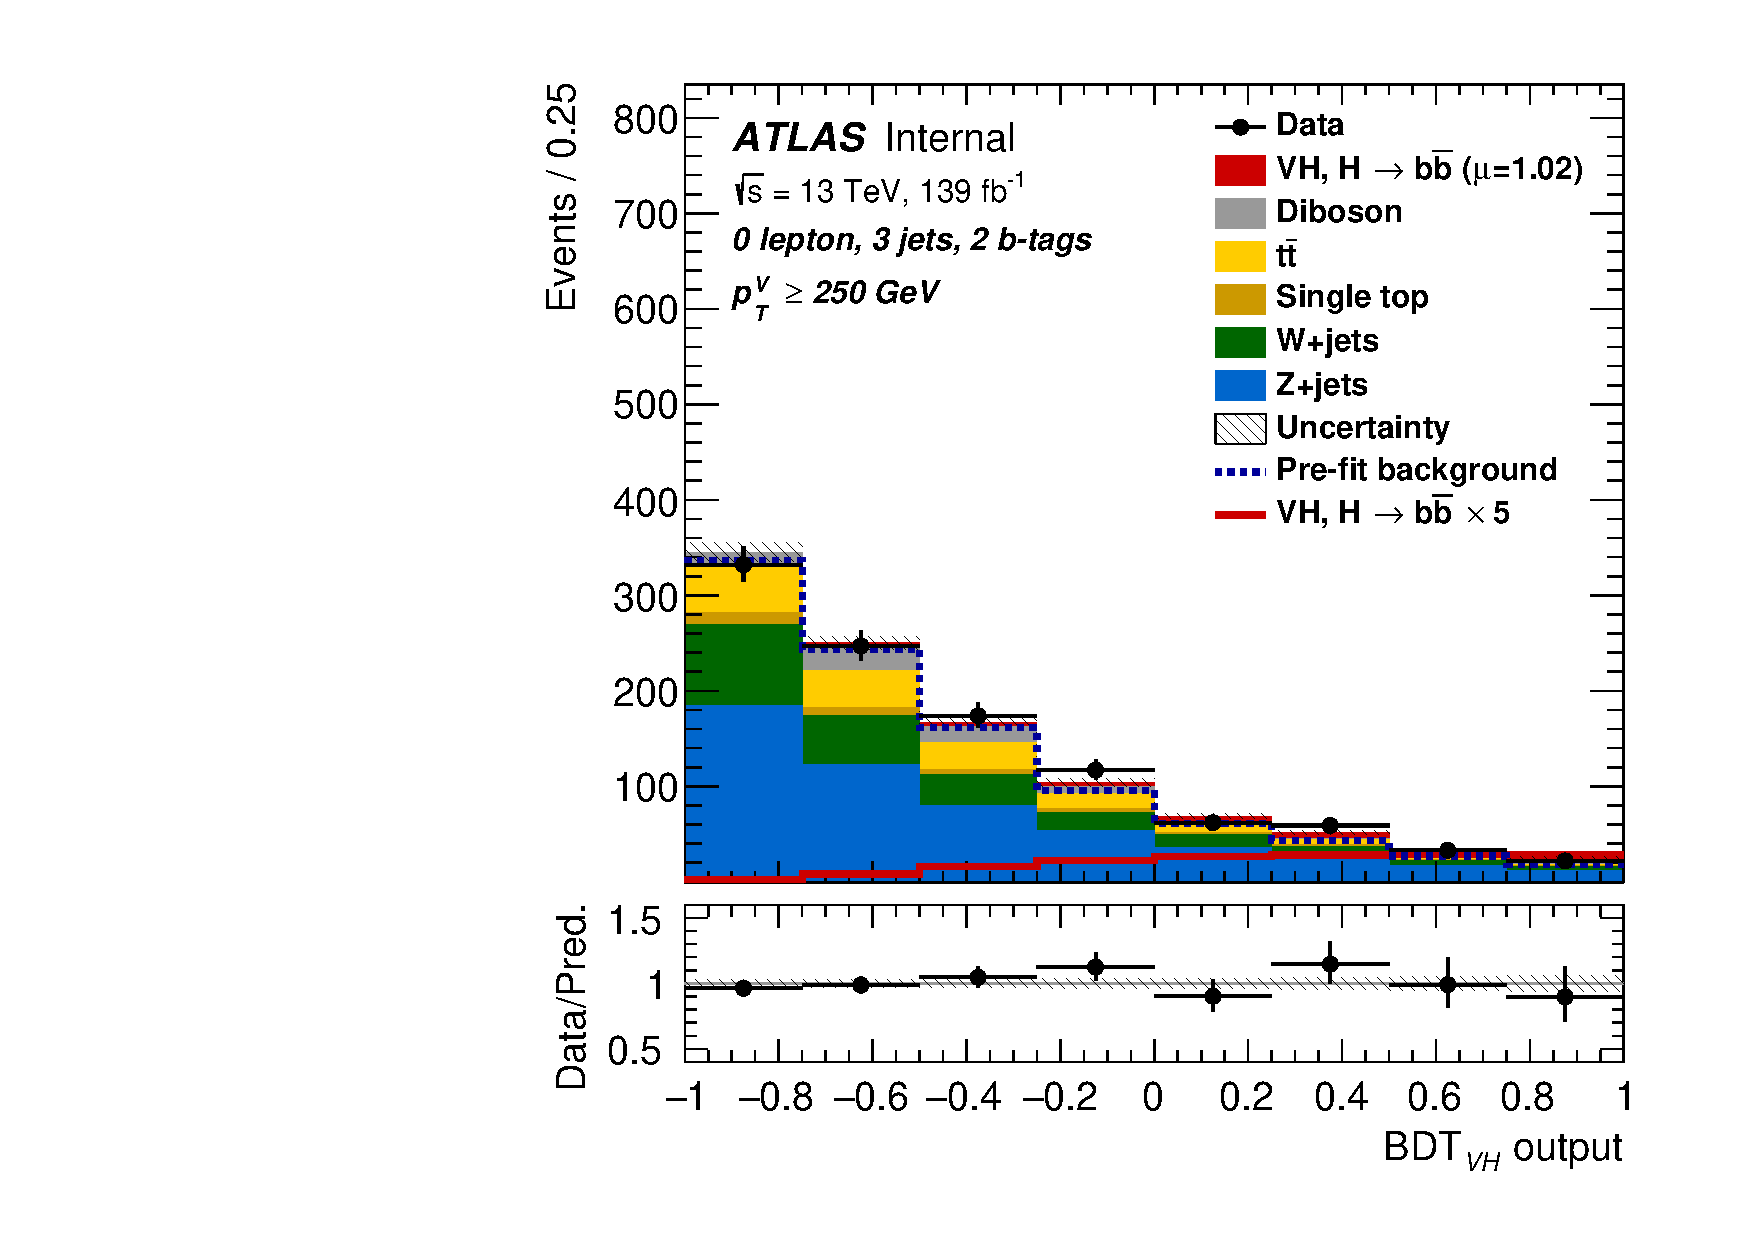
\includegraphics[width=.3\textwidth]{final_fit_mva/postfit/Region_BMin250_Y6051_DSR_T2_L0_distmva_J3_GlobalFit_unconditionnal_mu1} \\

    % bottom row
    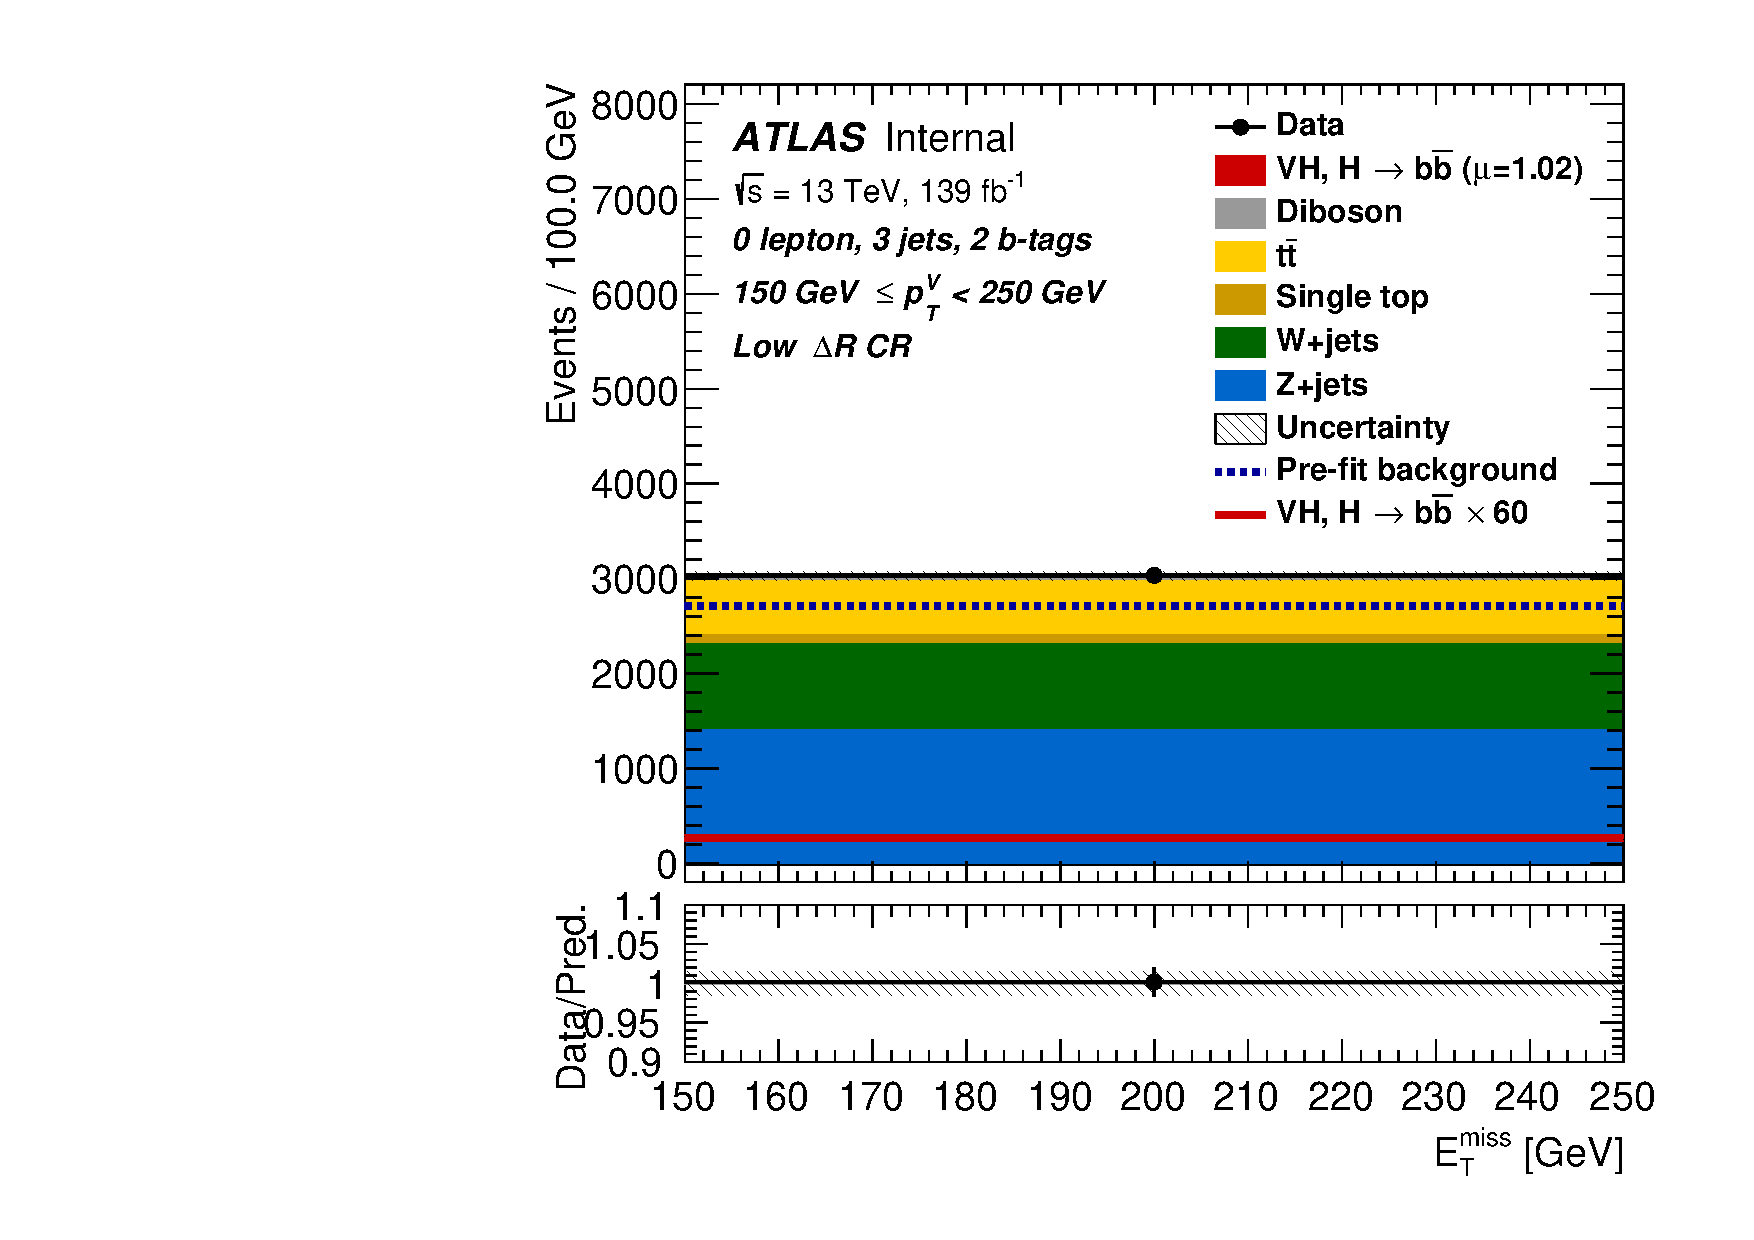
\includegraphics[width=.3\textwidth]{final_fit_mva/postfit/Region_BMax250_BMin150_Y6051_DCRLow_T2_L0_distMET_J3_GlobalFit_unconditionnal_mu1}%
    & 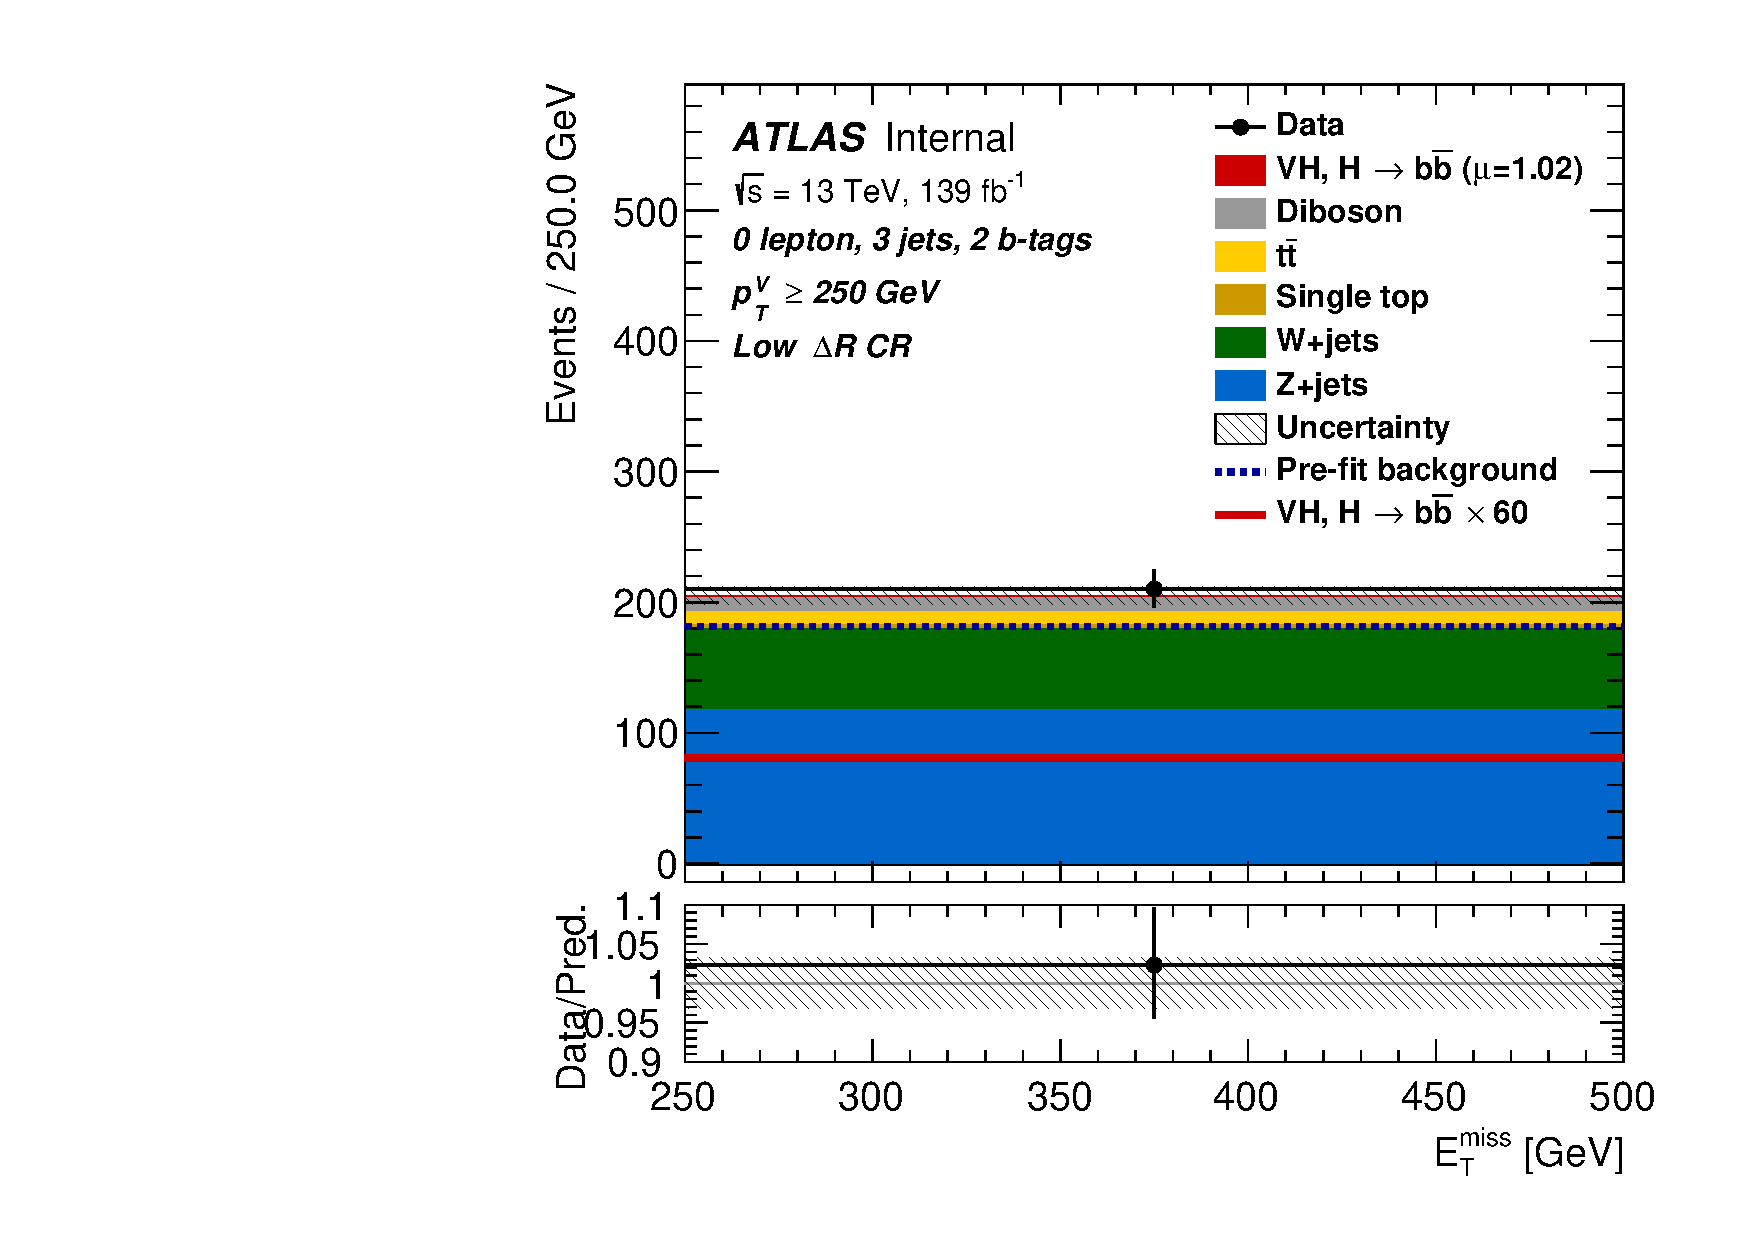
\includegraphics[width=.3\textwidth]{final_fit_mva/postfit/Region_BMin250_Y6051_DCRLow_T2_L0_distMET_J3_GlobalFit_unconditionnal_mu1} \\
  \end{tabular}
  \caption{Post-fit distributions in the 0 lepton 3 jet channel.}
\end{figure}
\begin{figure}
  \centering
  \begin{tabular}{cc}
    % top row
    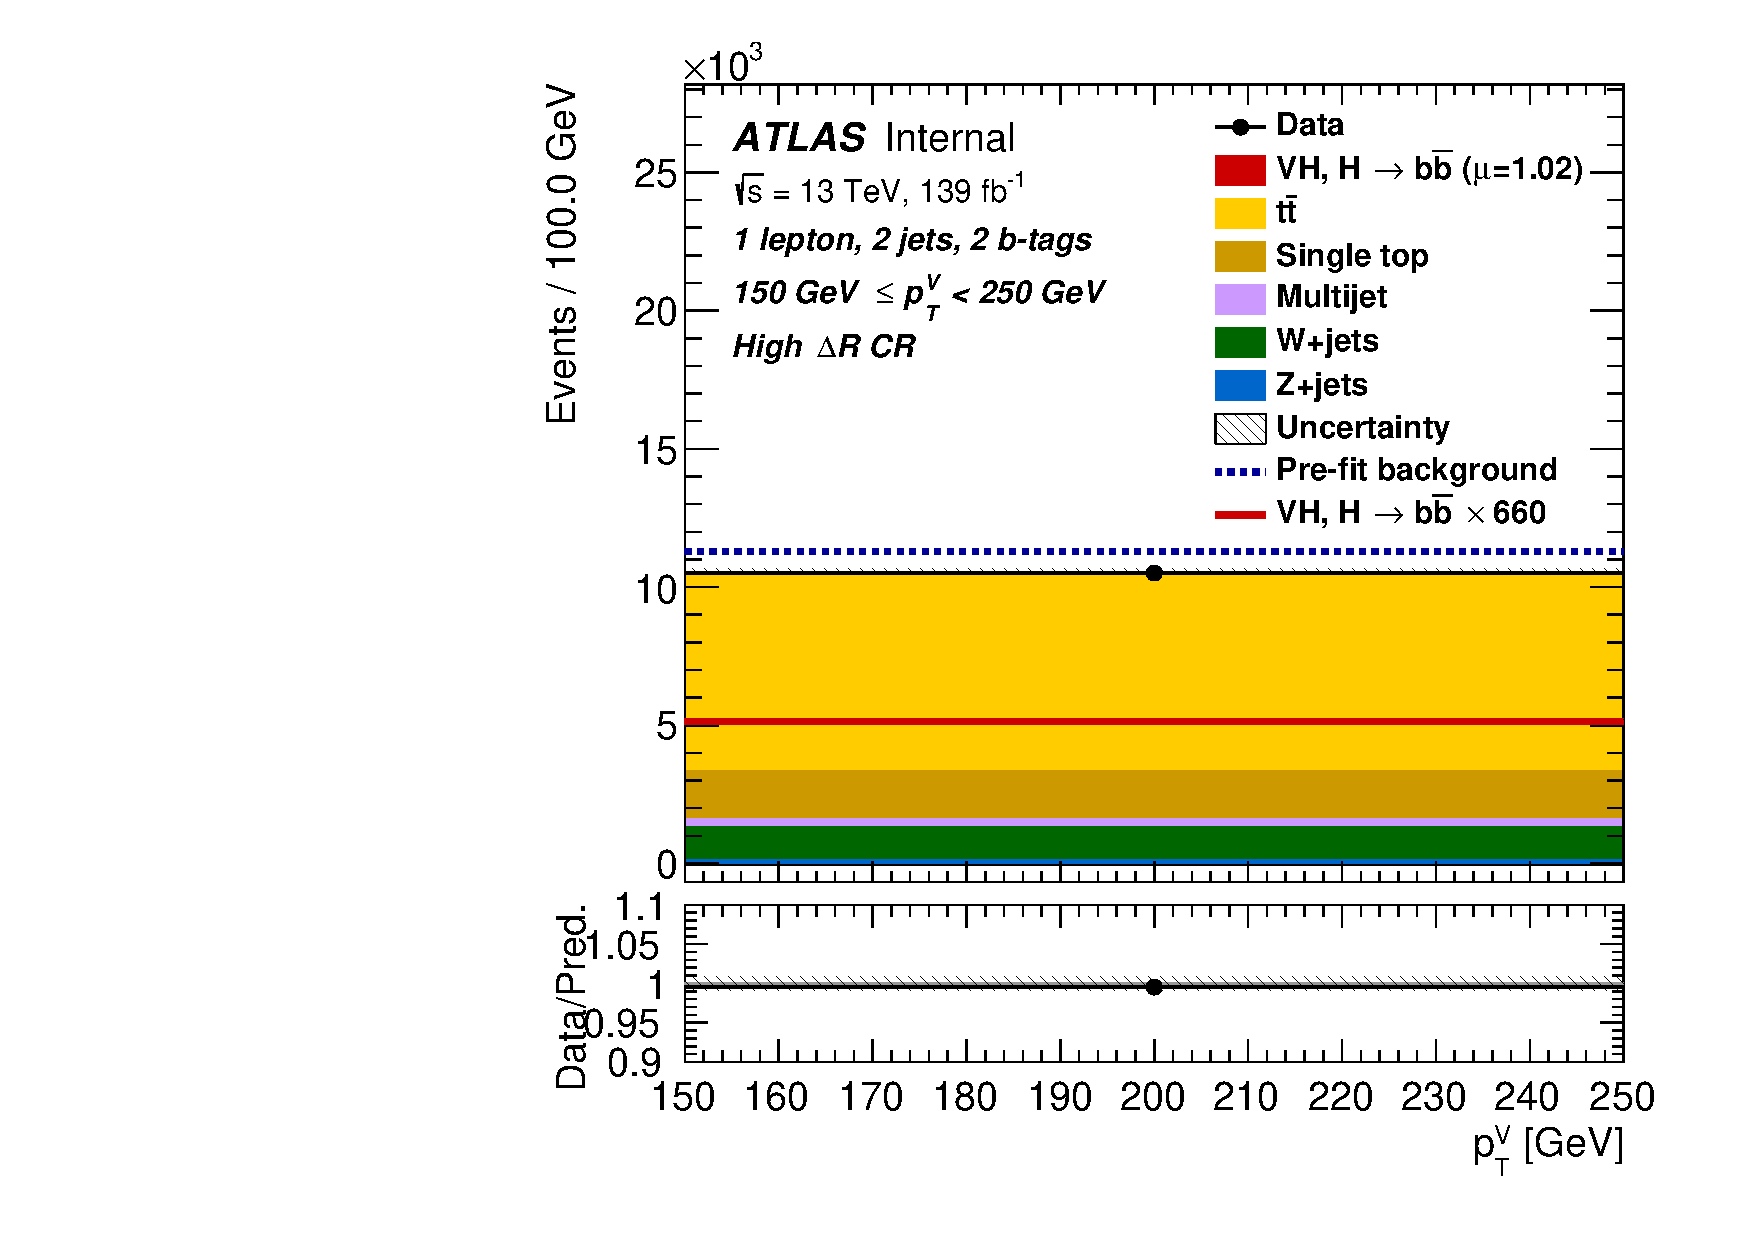
\includegraphics[width=.49\textwidth]{final_fit_mva/postfit/Region_BMax250_BMin150_Y6051_DCRHigh_T2_L1_distpTV_J2_GlobalFit_unconditionnal_mu1}%
    & 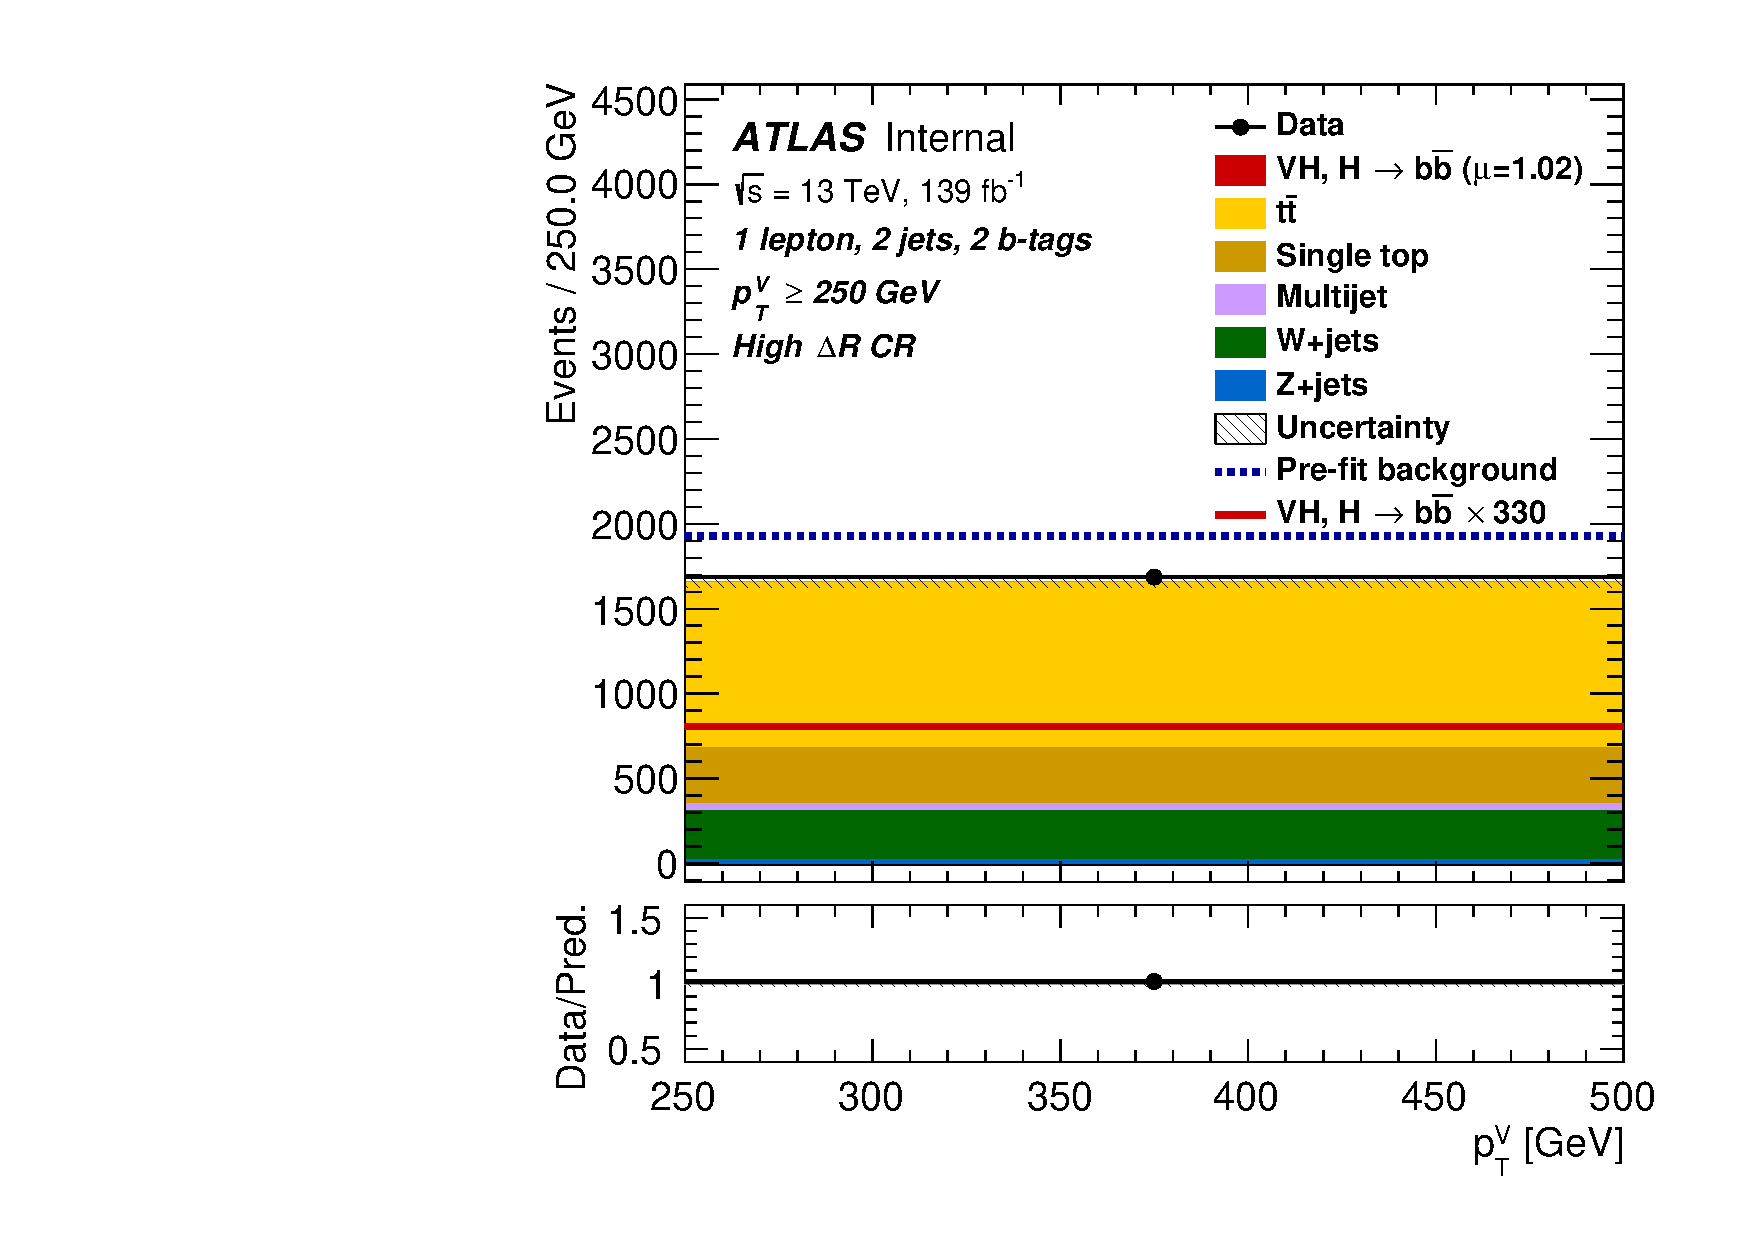
\includegraphics[width=.49\textwidth]{final_fit_mva/postfit/Region_BMin250_Y6051_DCRHigh_T2_L1_distpTV_J2_GlobalFit_unconditionnal_mu1} \\

    % middle row
    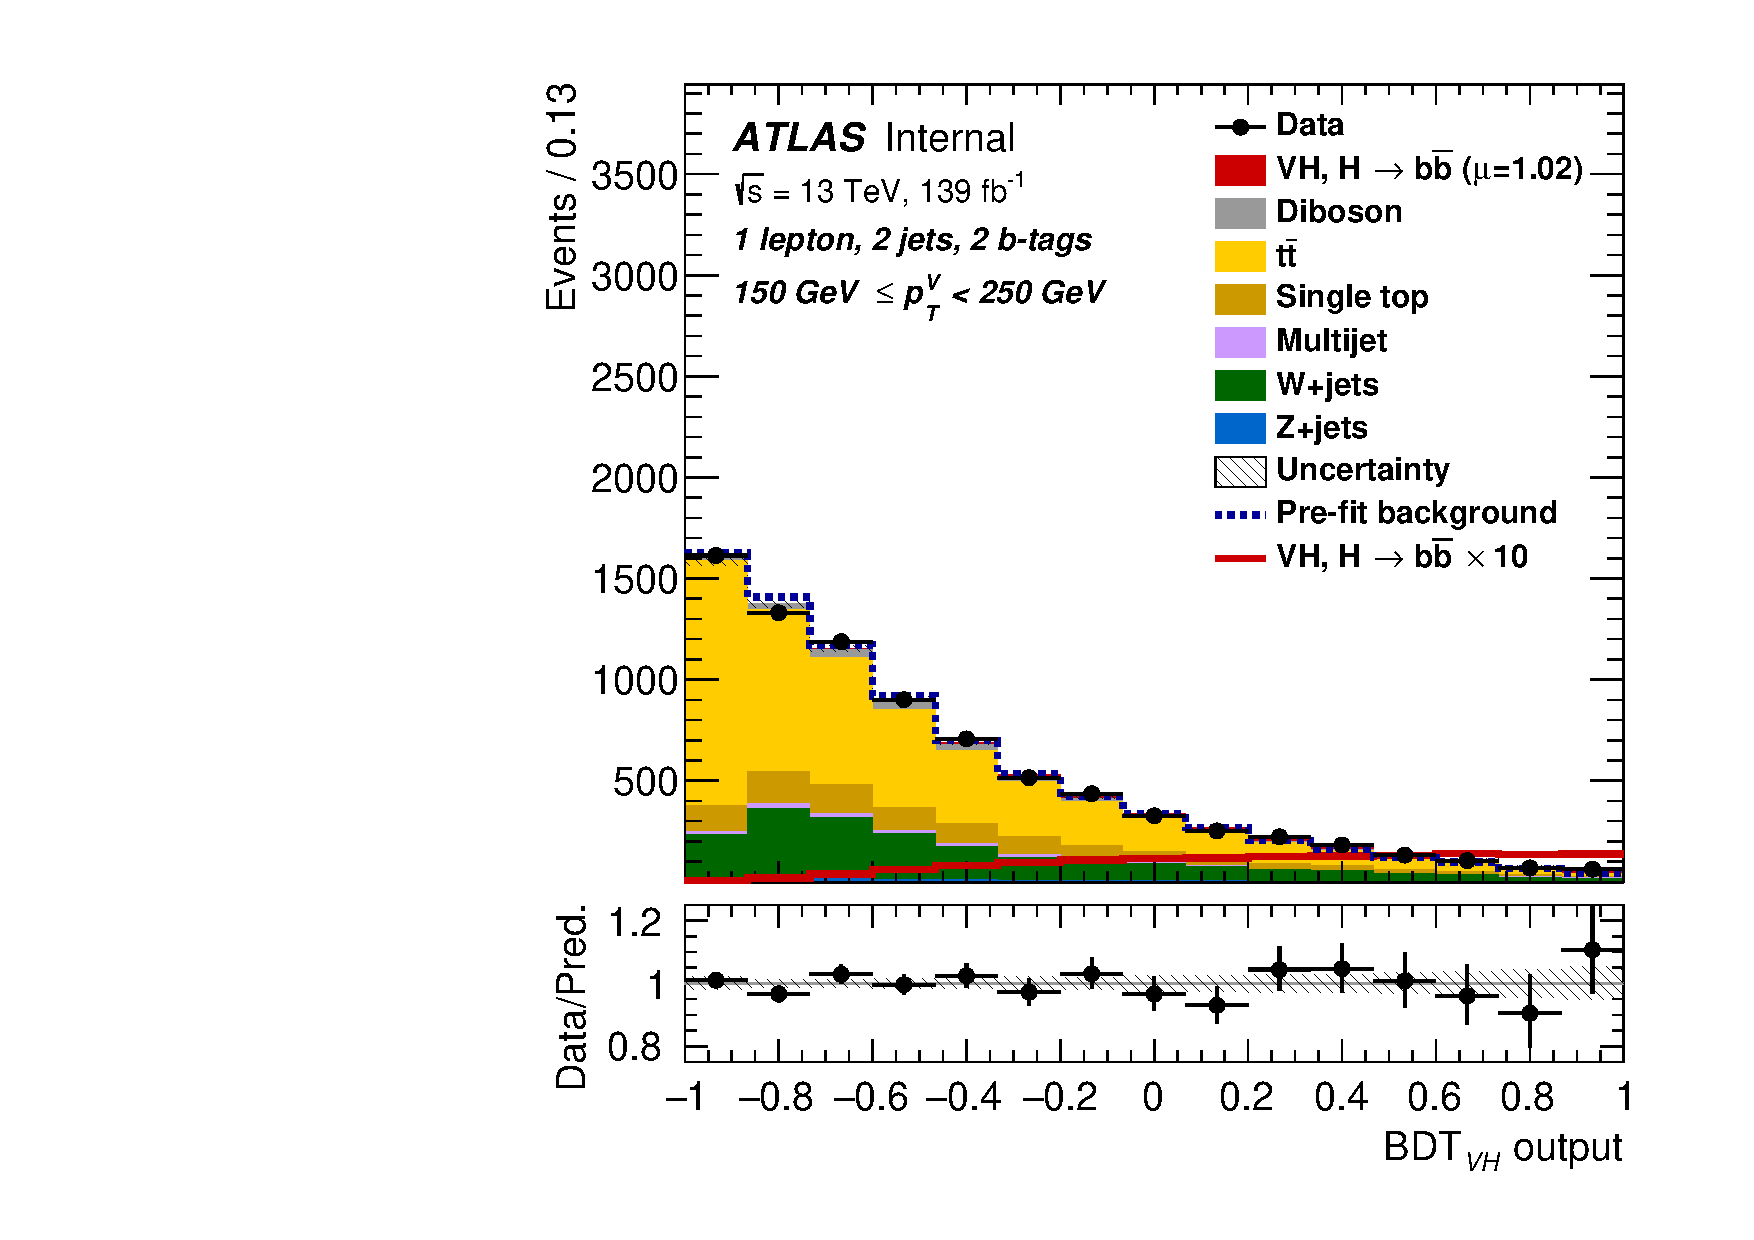
\includegraphics[width=.49\textwidth]{final_fit_mva/postfit/Region_BMax250_BMin150_Y6051_DSR_T2_L1_distmva_J2_GlobalFit_unconditionnal_mu1}%
    & 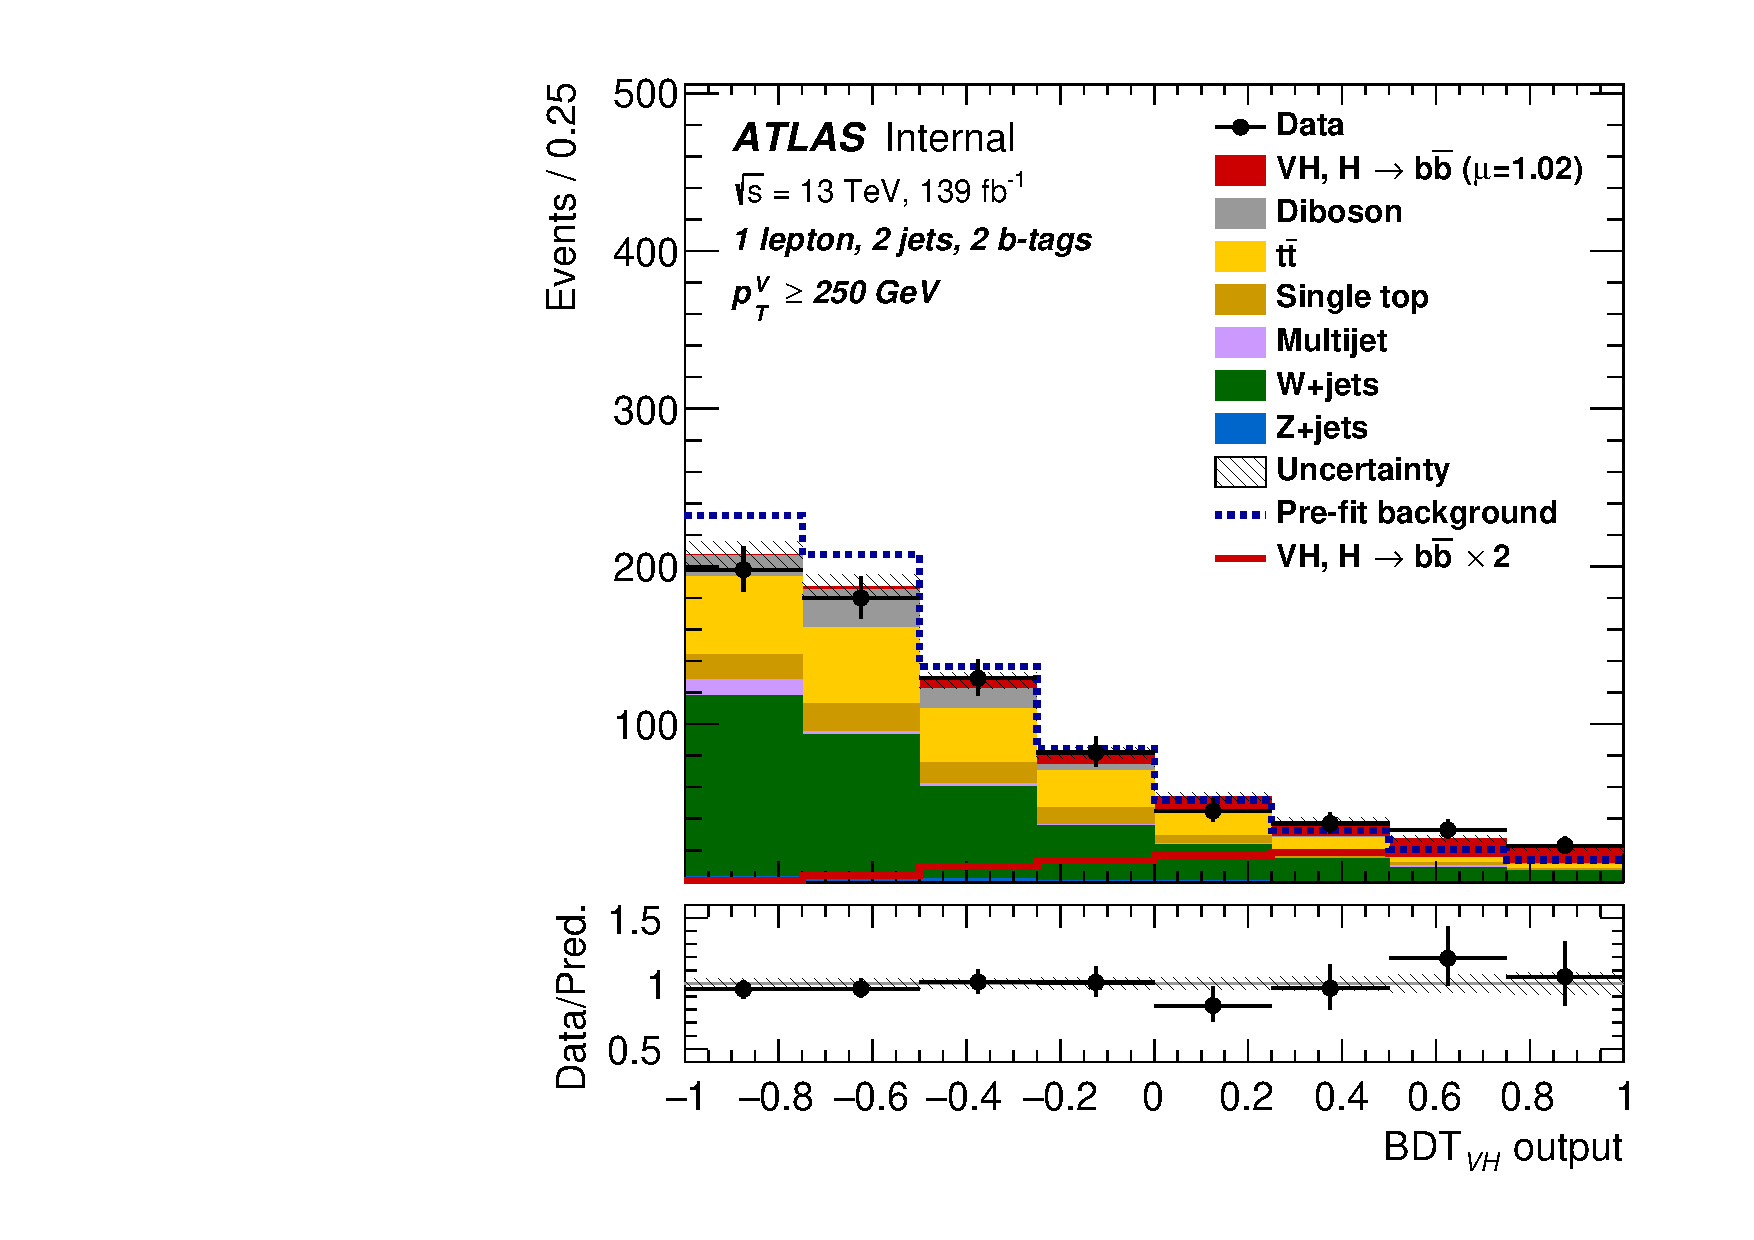
\includegraphics[width=.49\textwidth]{final_fit_mva/postfit/Region_BMin250_Y6051_DSR_T2_L1_distmva_J2_GlobalFit_unconditionnal_mu1} \\

    % bottom row
    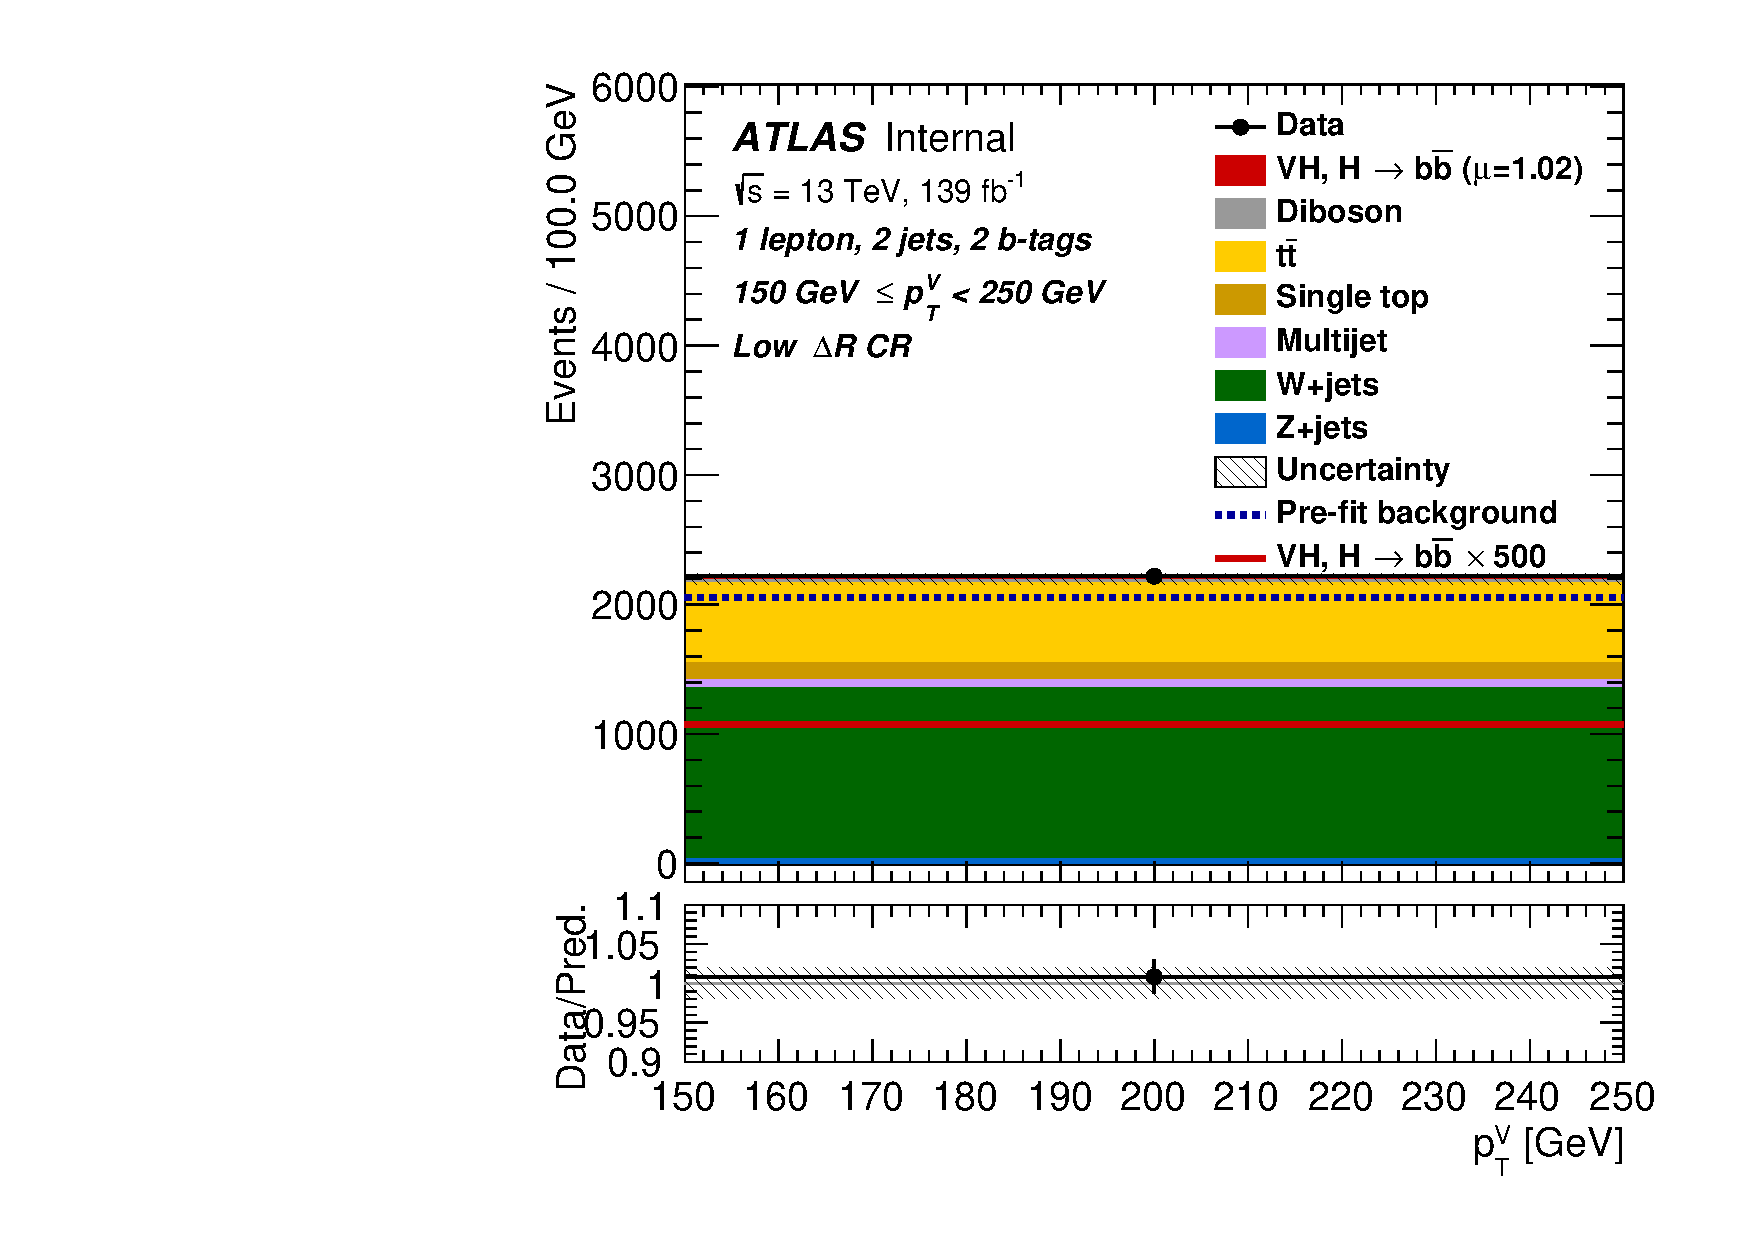
\includegraphics[width=.49\textwidth]{final_fit_mva/postfit/Region_BMax250_BMin150_Y6051_DCRLow_T2_L1_distpTV_J2_GlobalFit_unconditionnal_mu1}%
    & 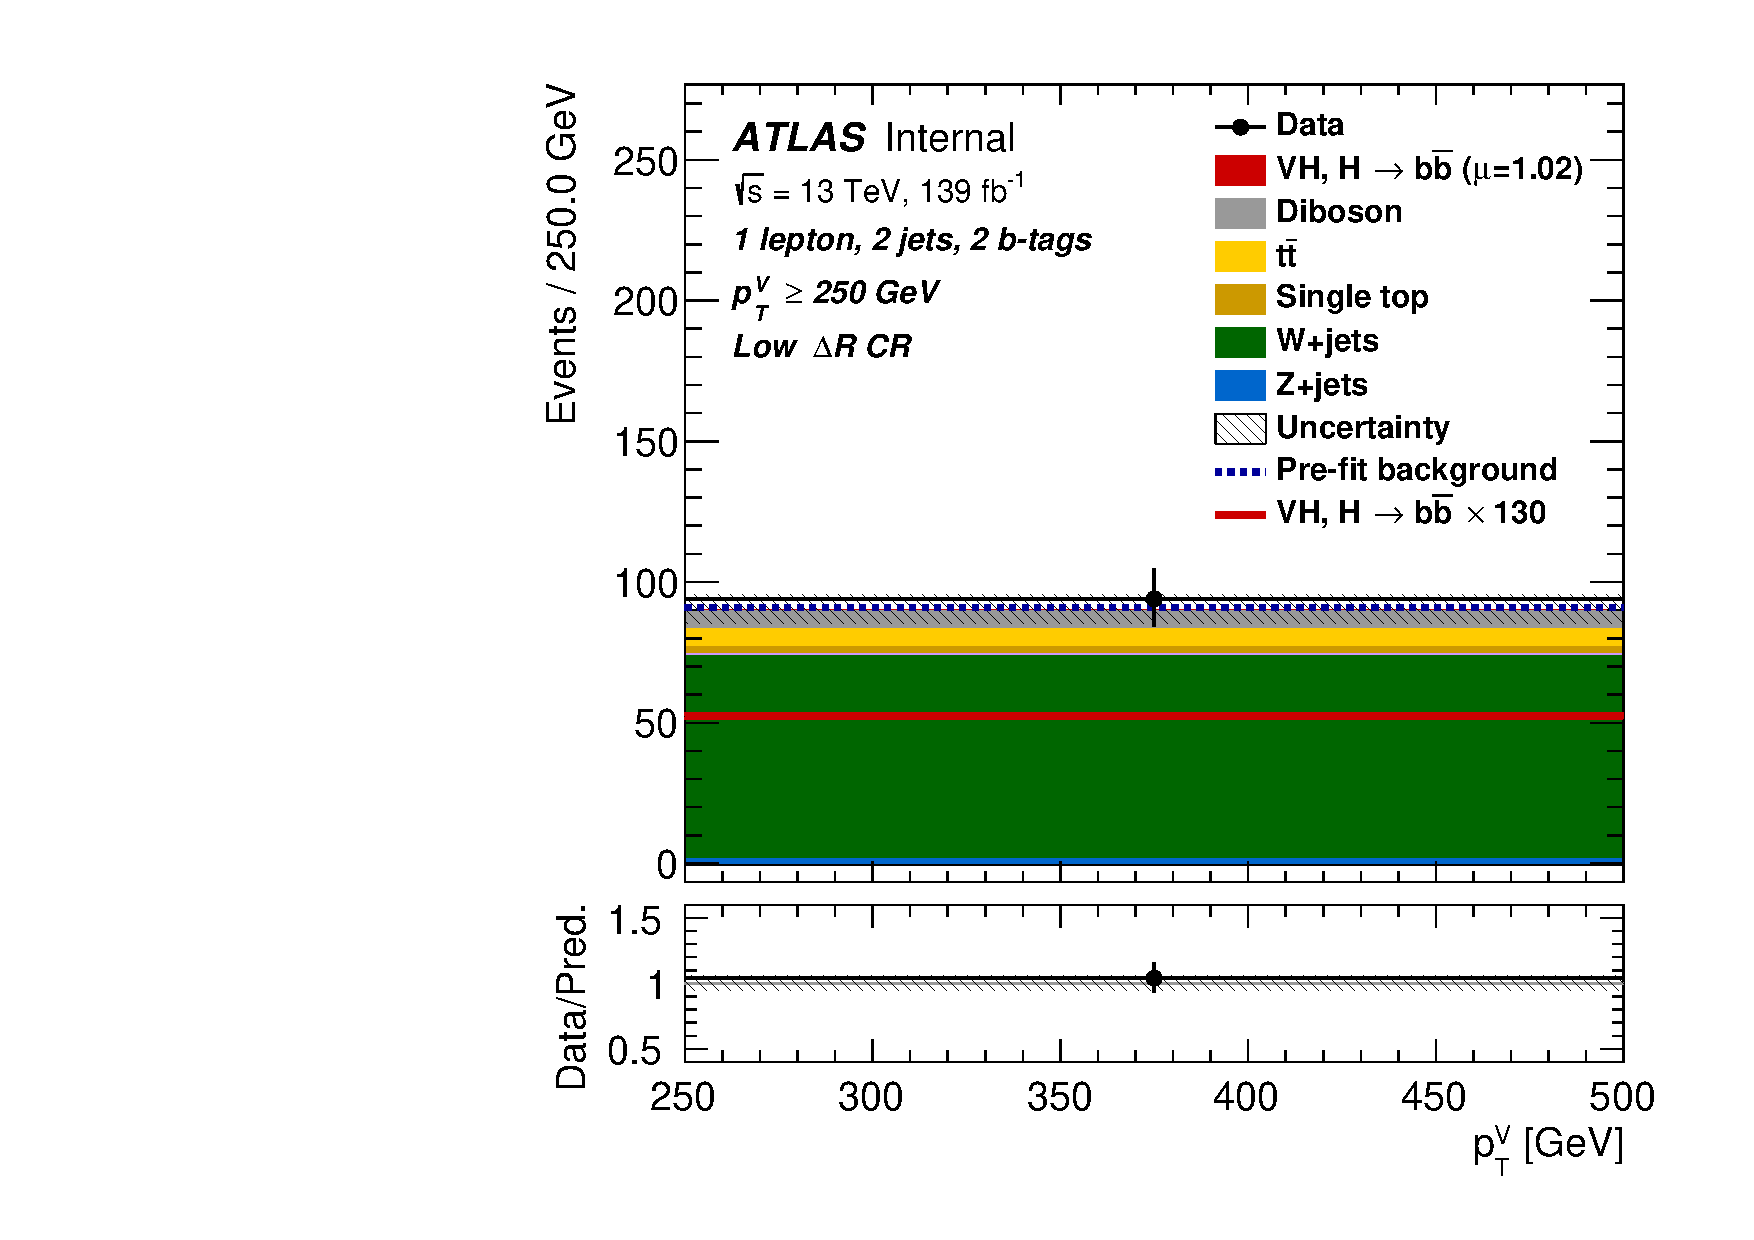
\includegraphics[width=.49\textwidth]{final_fit_mva/postfit/Region_BMin250_Y6051_DCRLow_T2_L1_distpTV_J2_GlobalFit_unconditionnal_mu1} \\
  \end{tabular}
  \caption{Post-fit distributions in the 1--lepton 2--jet channel.}
\end{figure}
\begin{figure}
  \centering
  \begin{tabular}{cc}
    % top row
    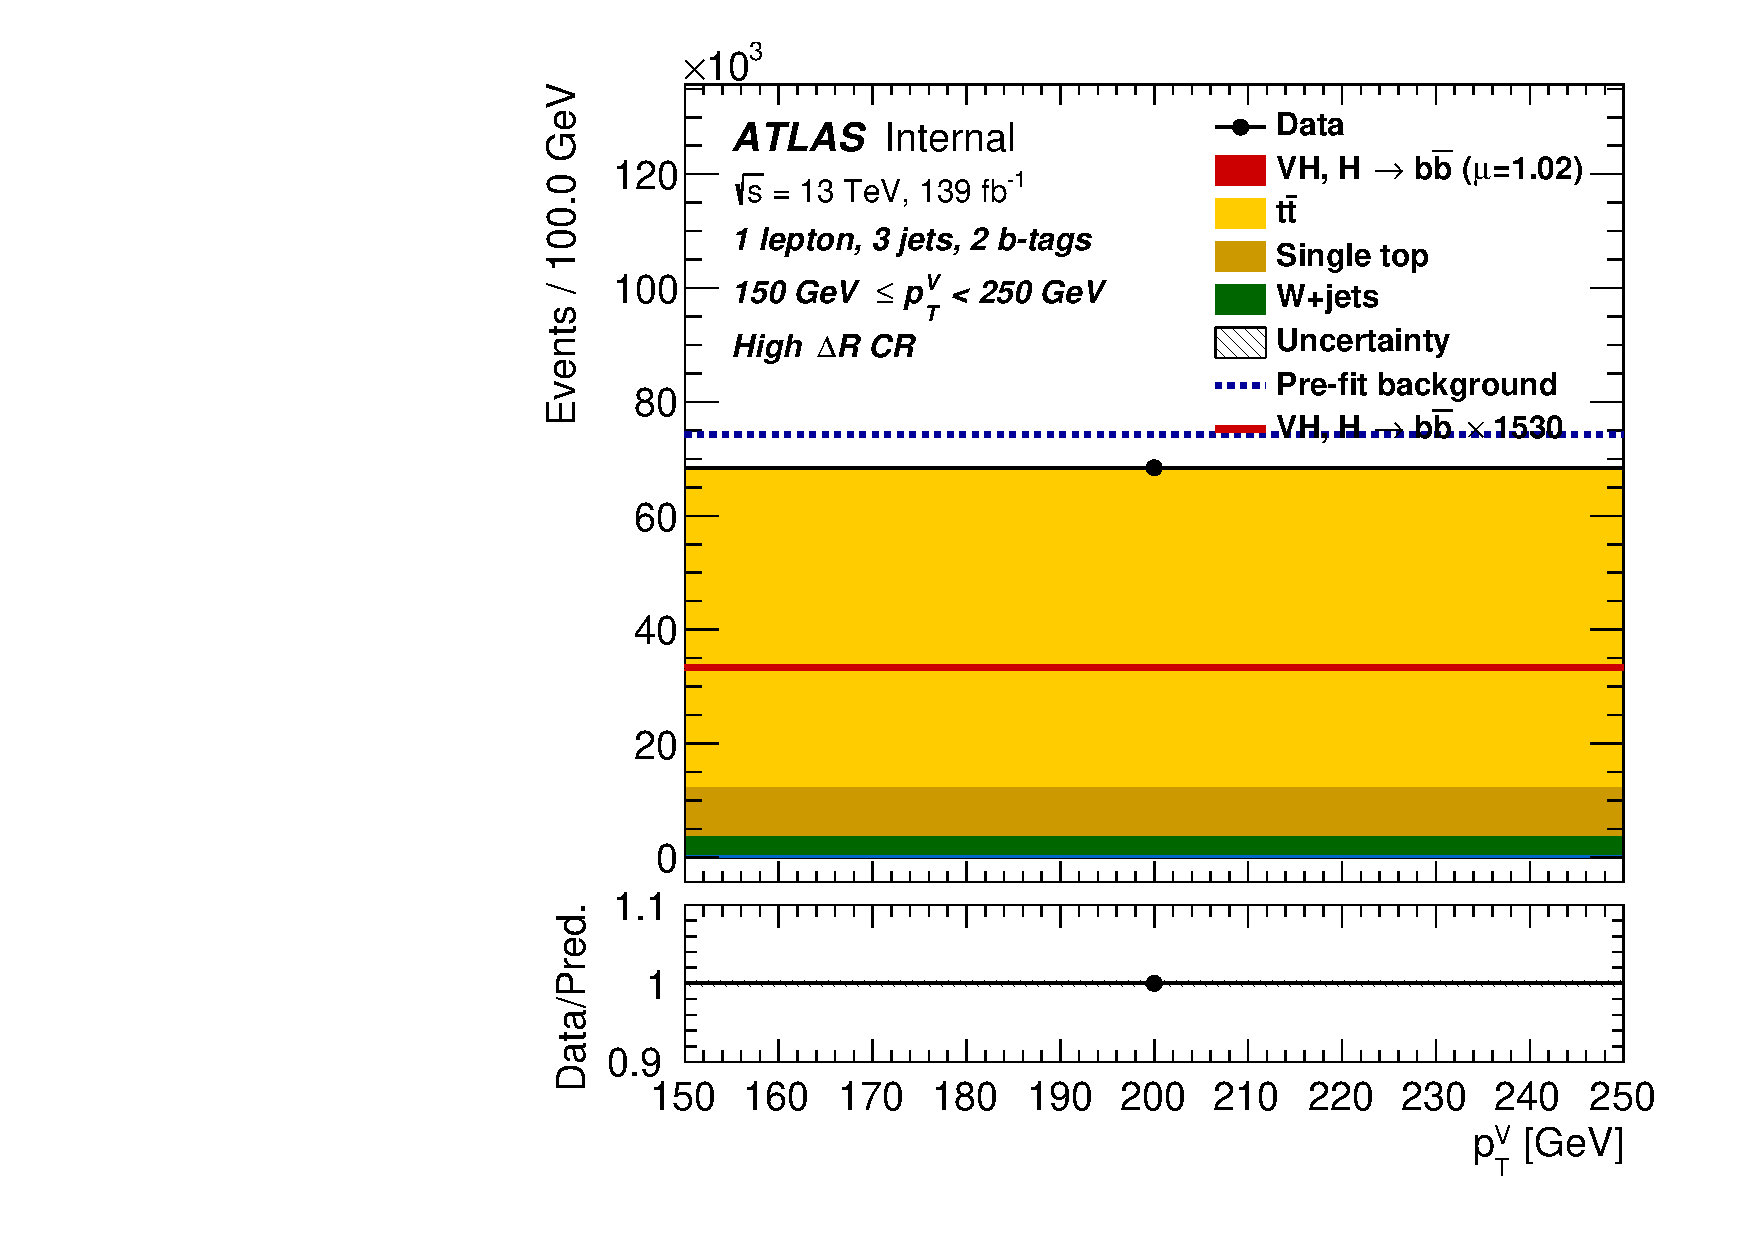
\includegraphics[width=.3\textwidth]{final_fit_mva/postfit/Region_BMax250_BMin150_Y6051_DCRHigh_T2_L1_distpTV_J3_GlobalFit_unconditionnal_mu1}%
    & 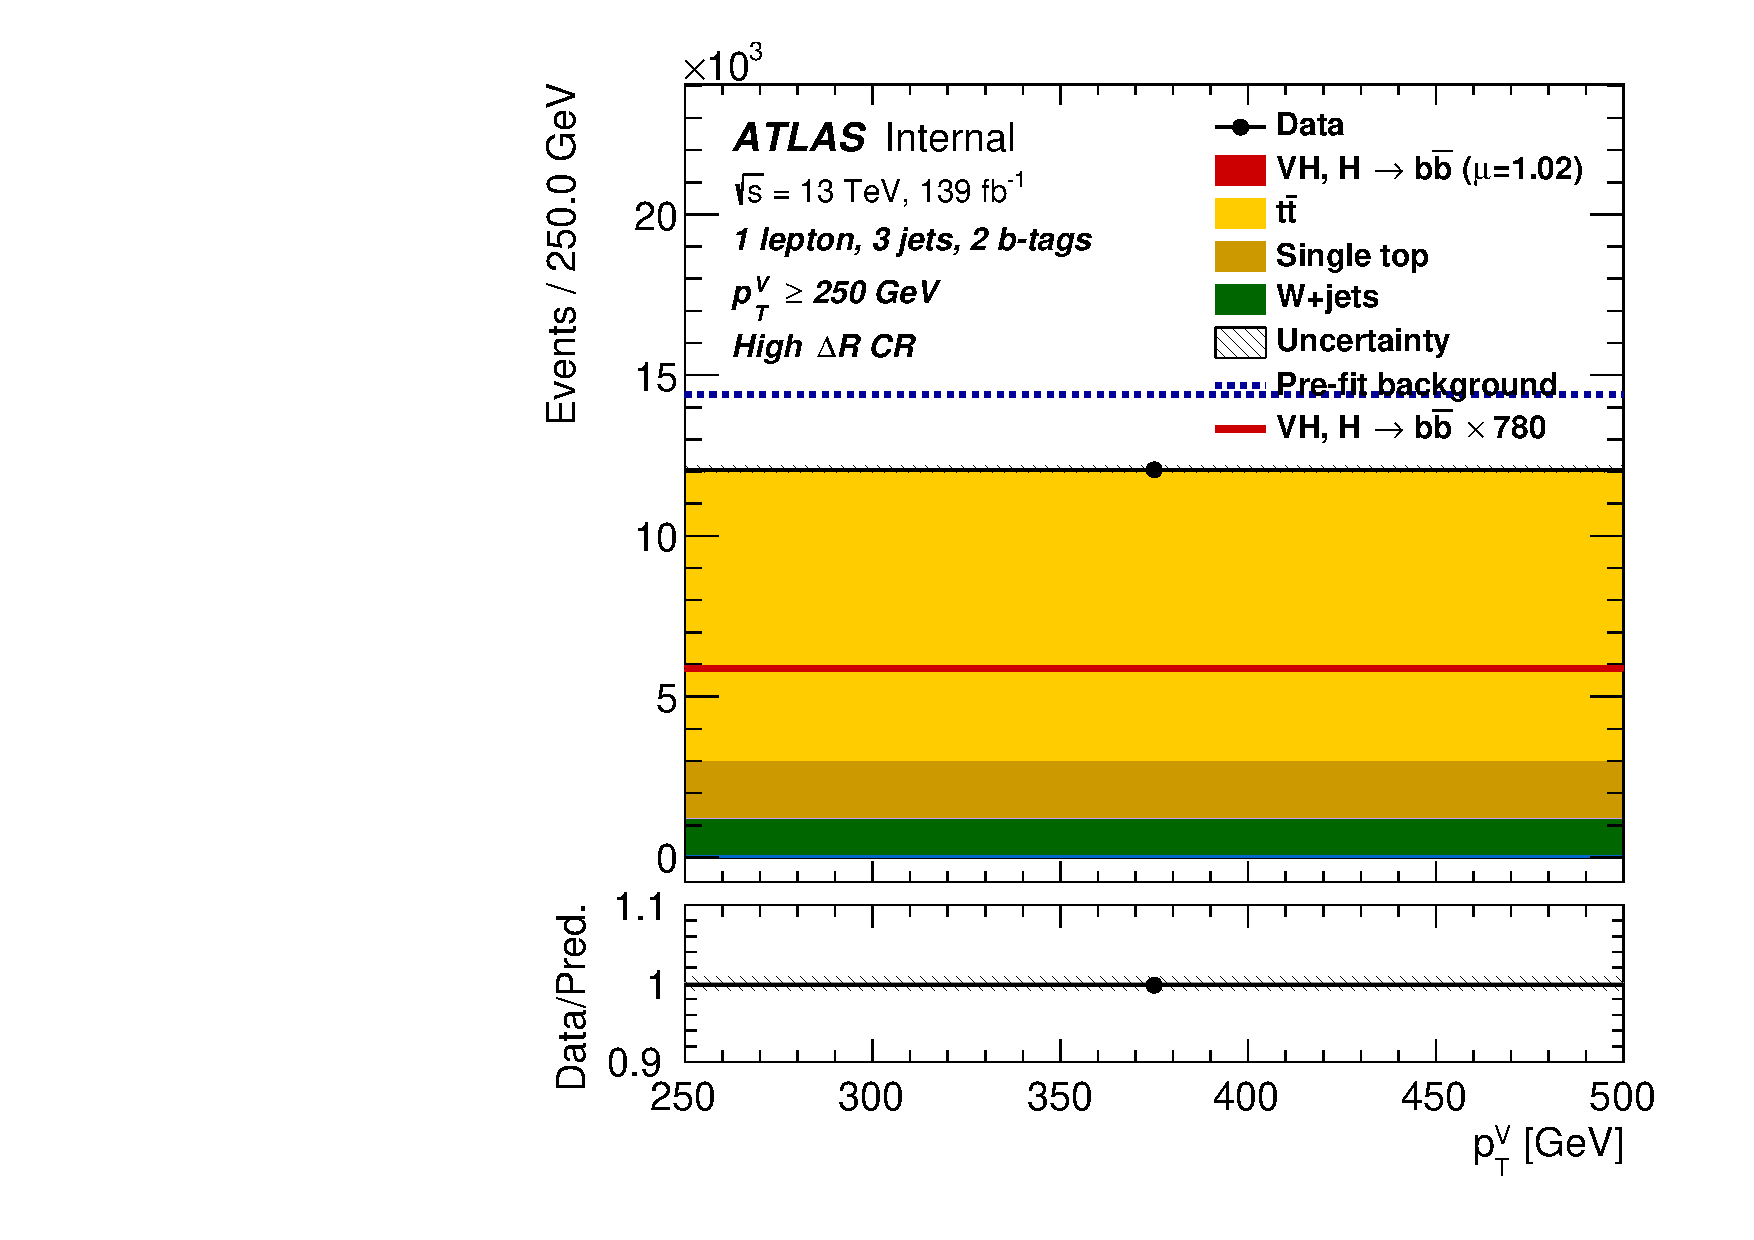
\includegraphics[width=.3\textwidth]{final_fit_mva/postfit/Region_BMin250_Y6051_DCRHigh_T2_L1_distpTV_J3_GlobalFit_unconditionnal_mu1} \\

    % middle row
    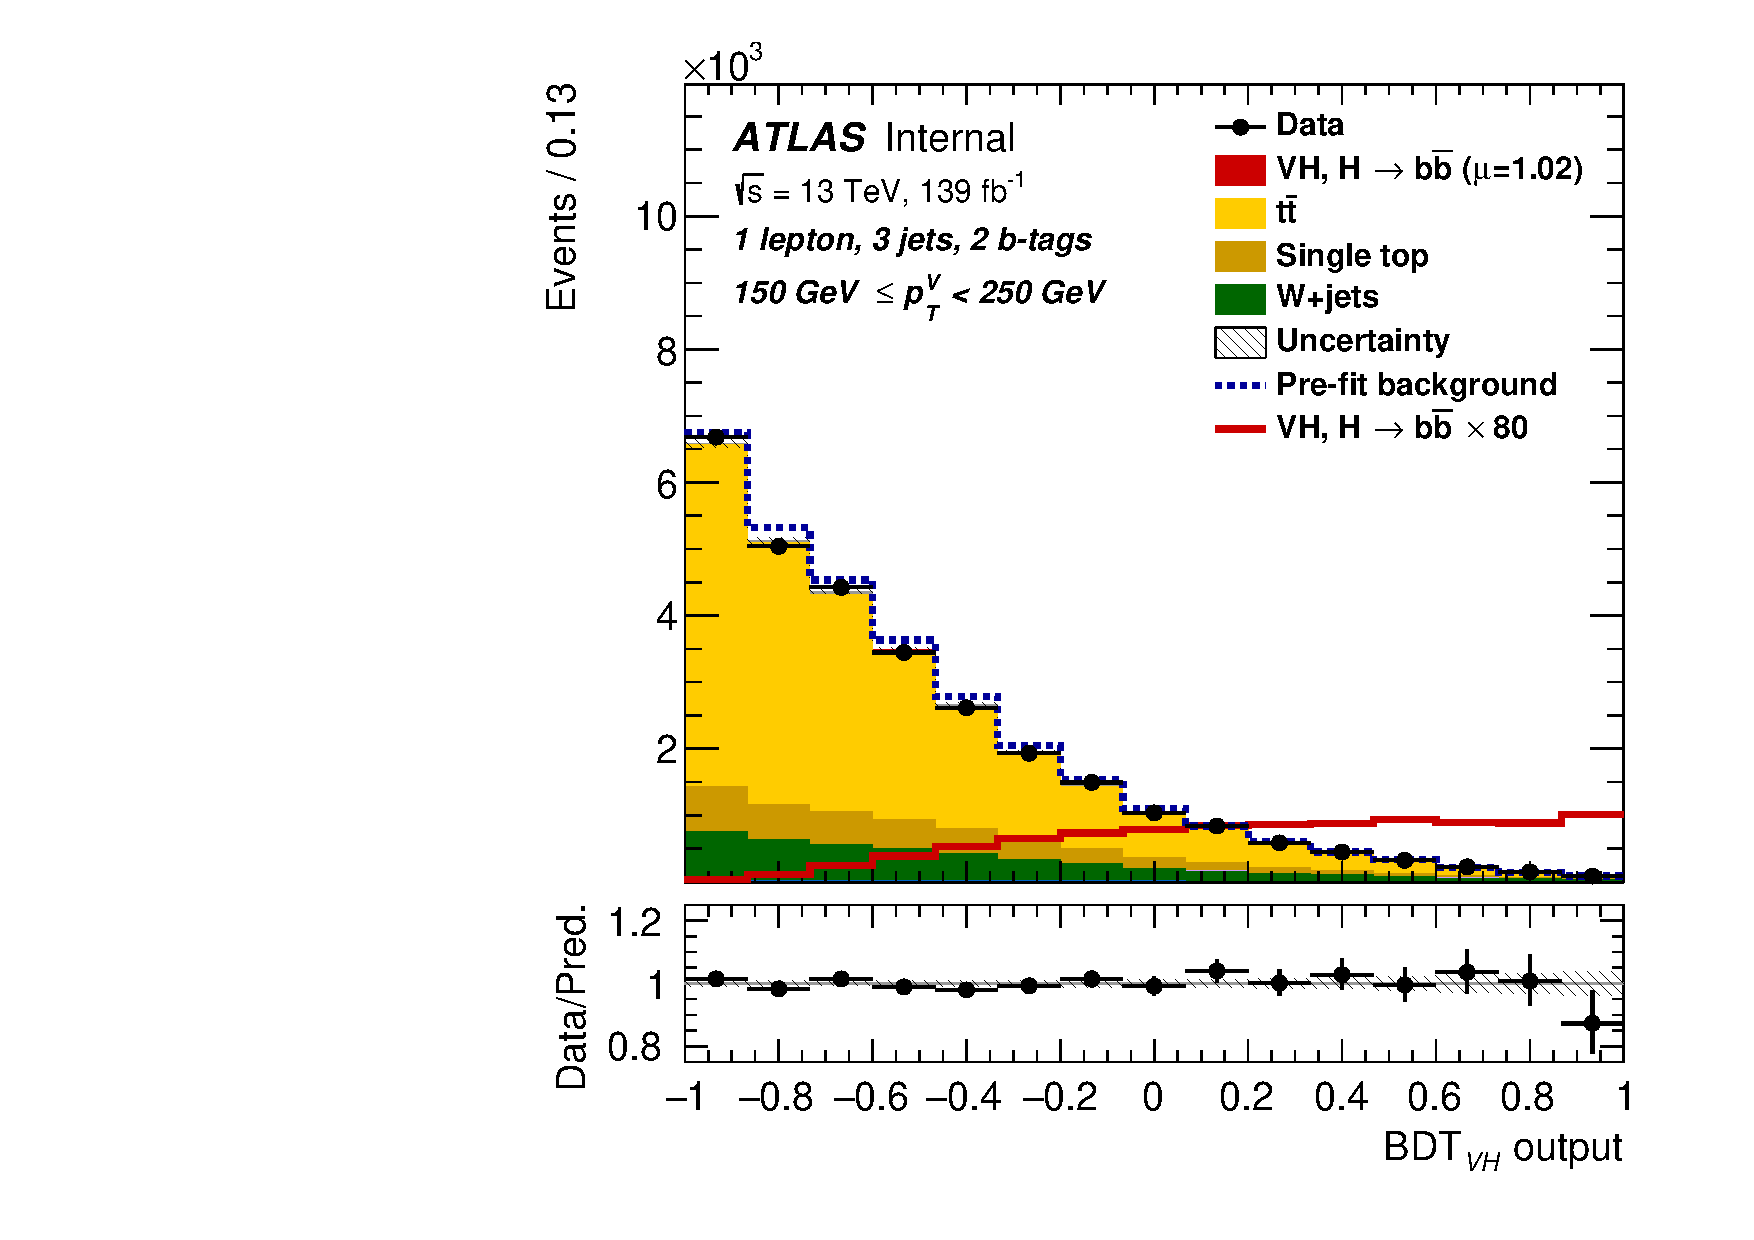
\includegraphics[width=.3\textwidth]{final_fit_mva/postfit/Region_BMax250_BMin150_Y6051_DSR_T2_L1_distmva_J3_GlobalFit_unconditionnal_mu1}%
    & 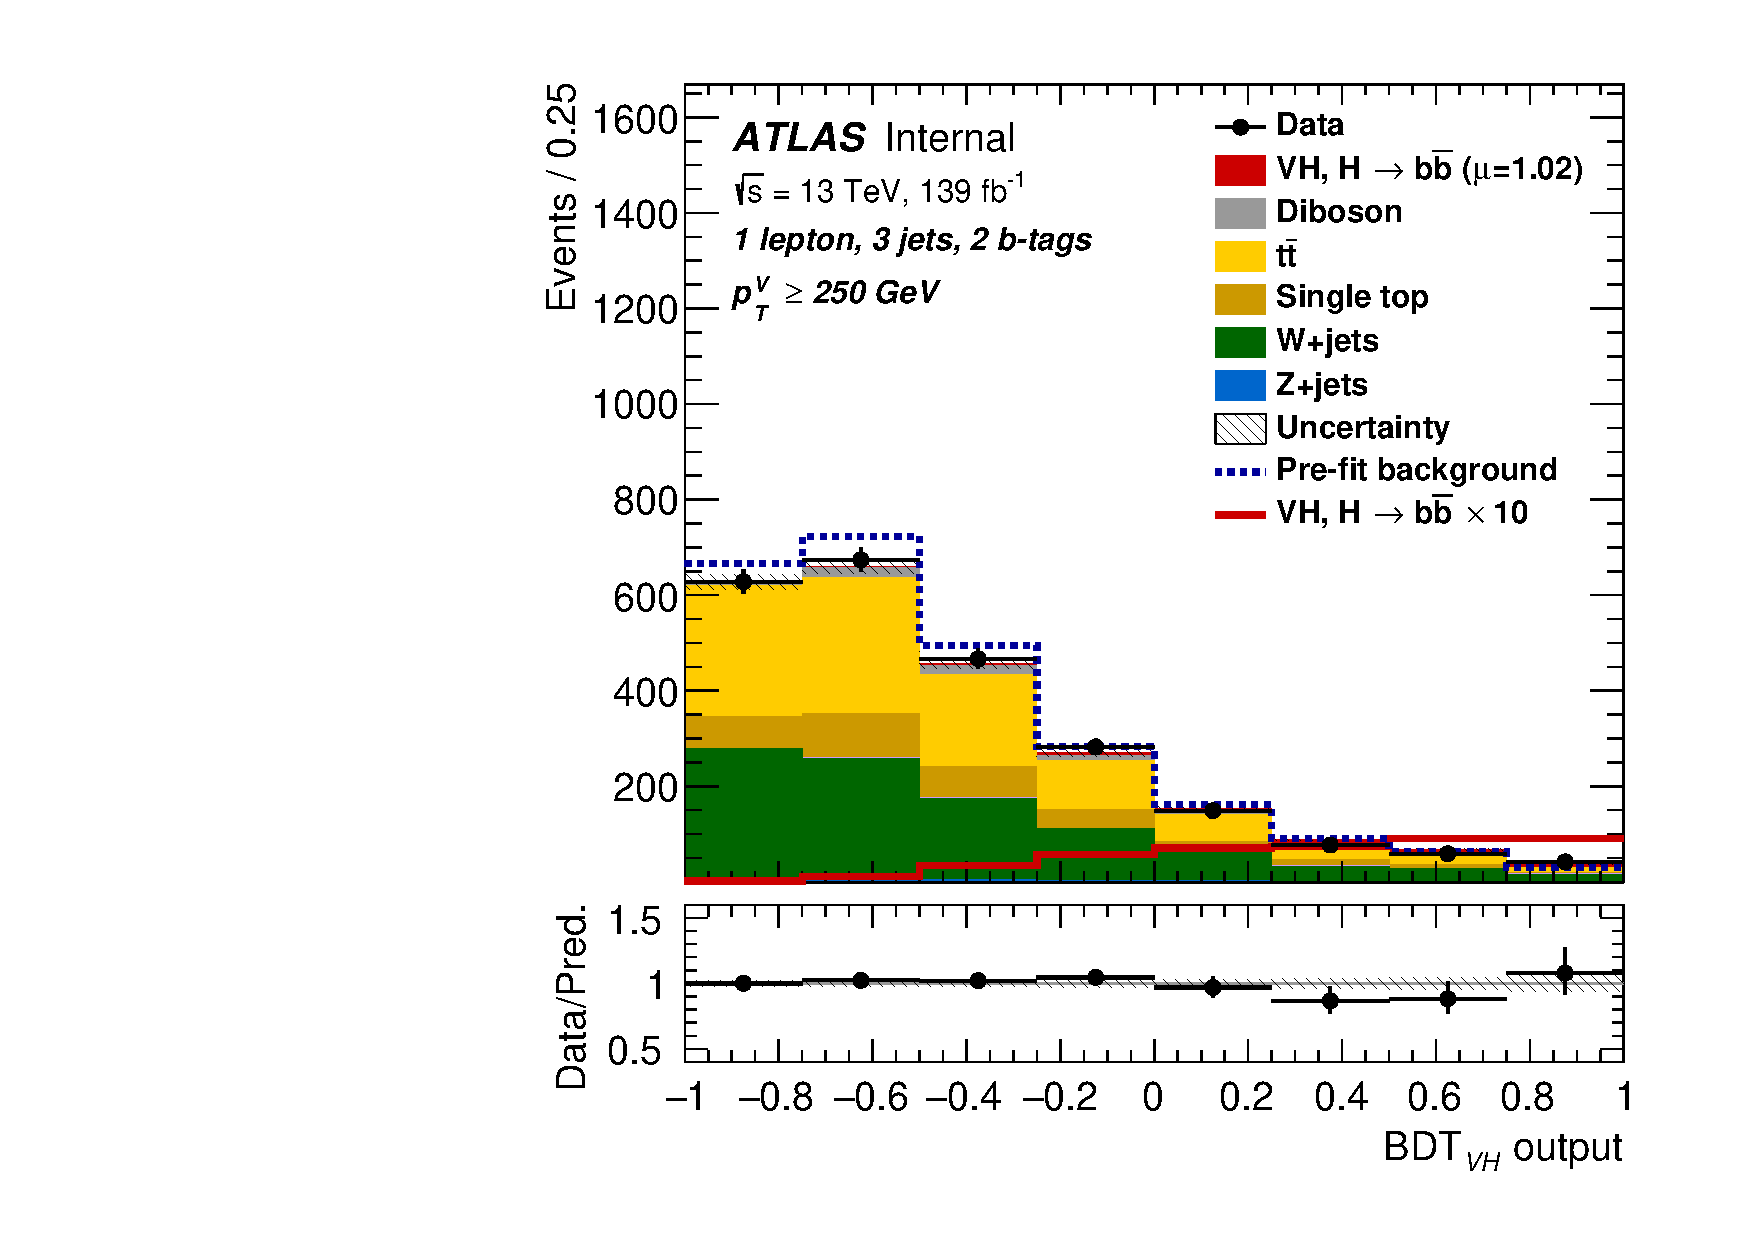
\includegraphics[width=.3\textwidth]{final_fit_mva/postfit/Region_BMin250_Y6051_DSR_T2_L1_distmva_J3_GlobalFit_unconditionnal_mu1} \\

    % bottom row
    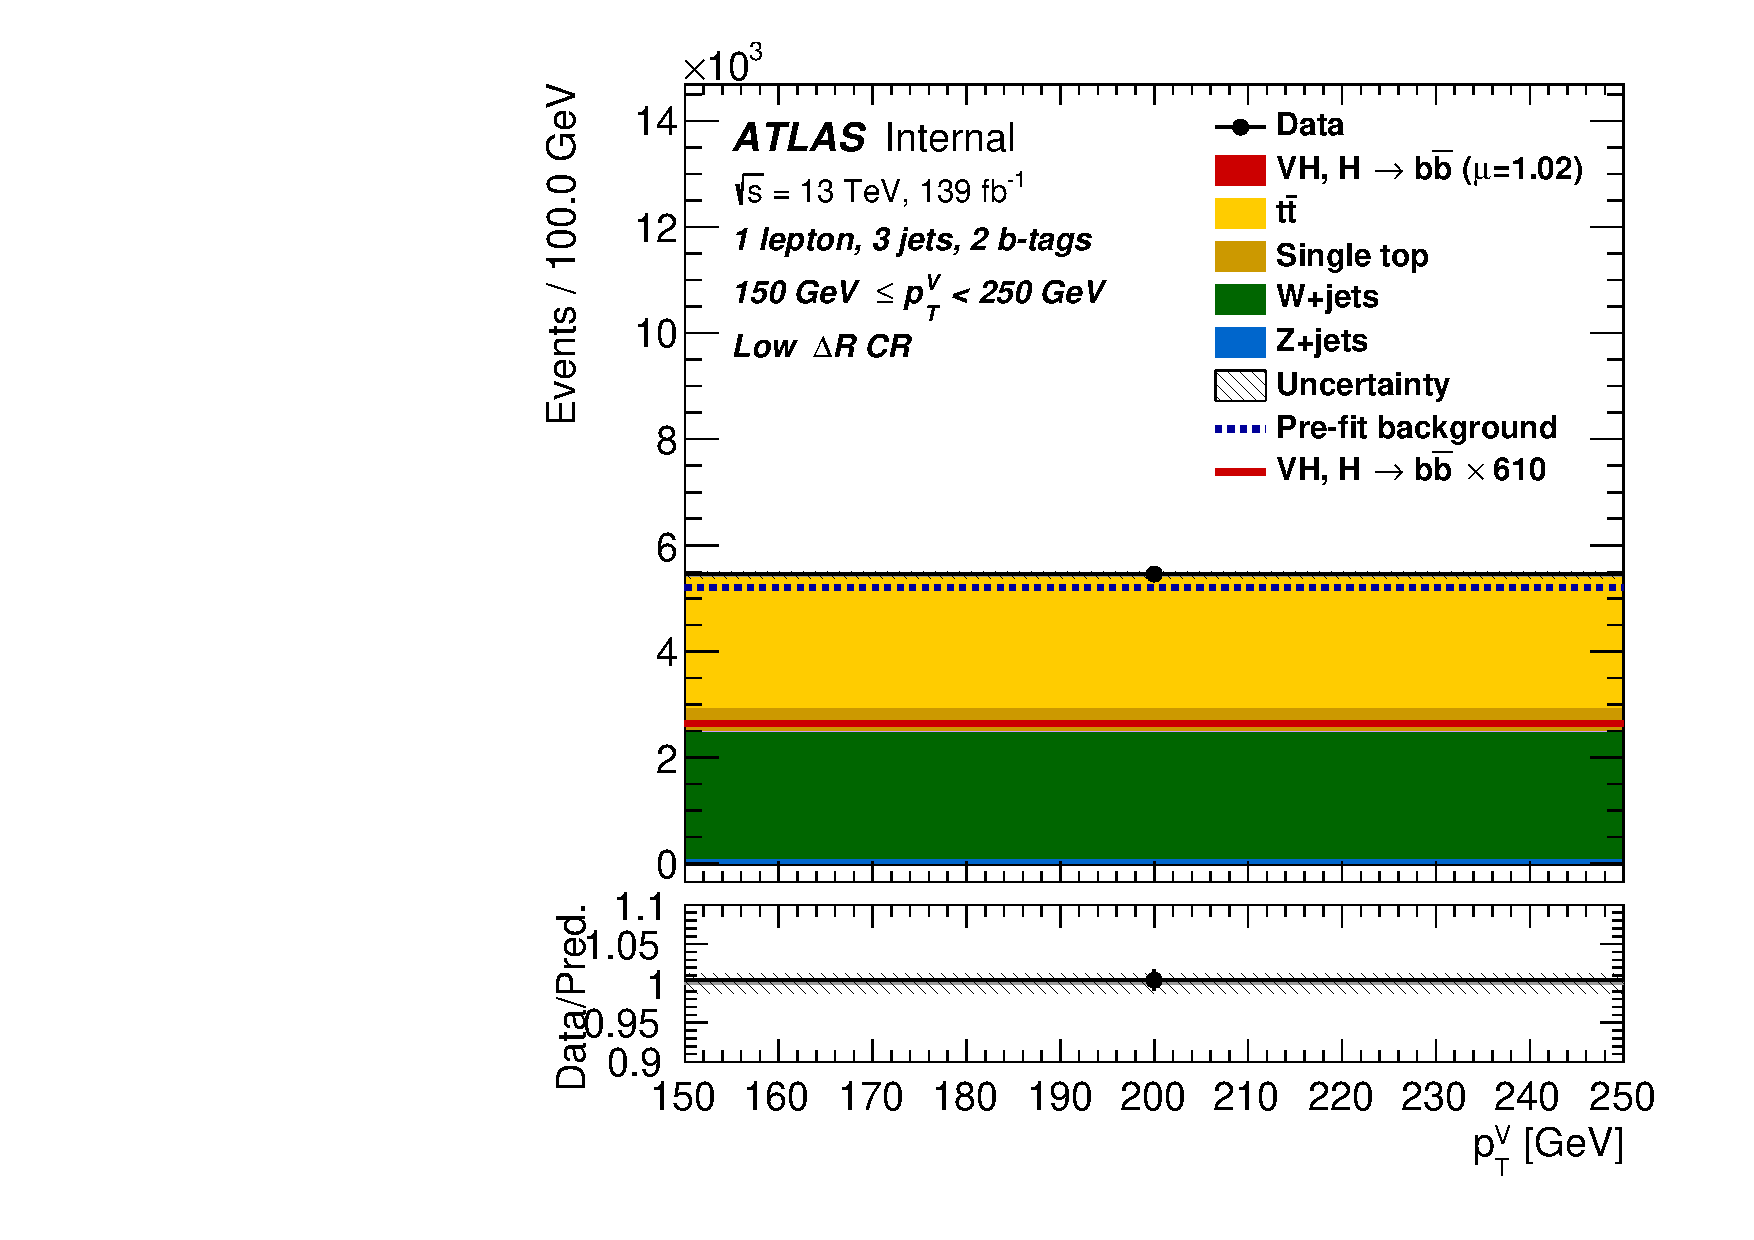
\includegraphics[width=.3\textwidth]{final_fit_mva/postfit/Region_BMax250_BMin150_Y6051_DCRLow_T2_L1_distpTV_J3_GlobalFit_unconditionnal_mu1}%
    & 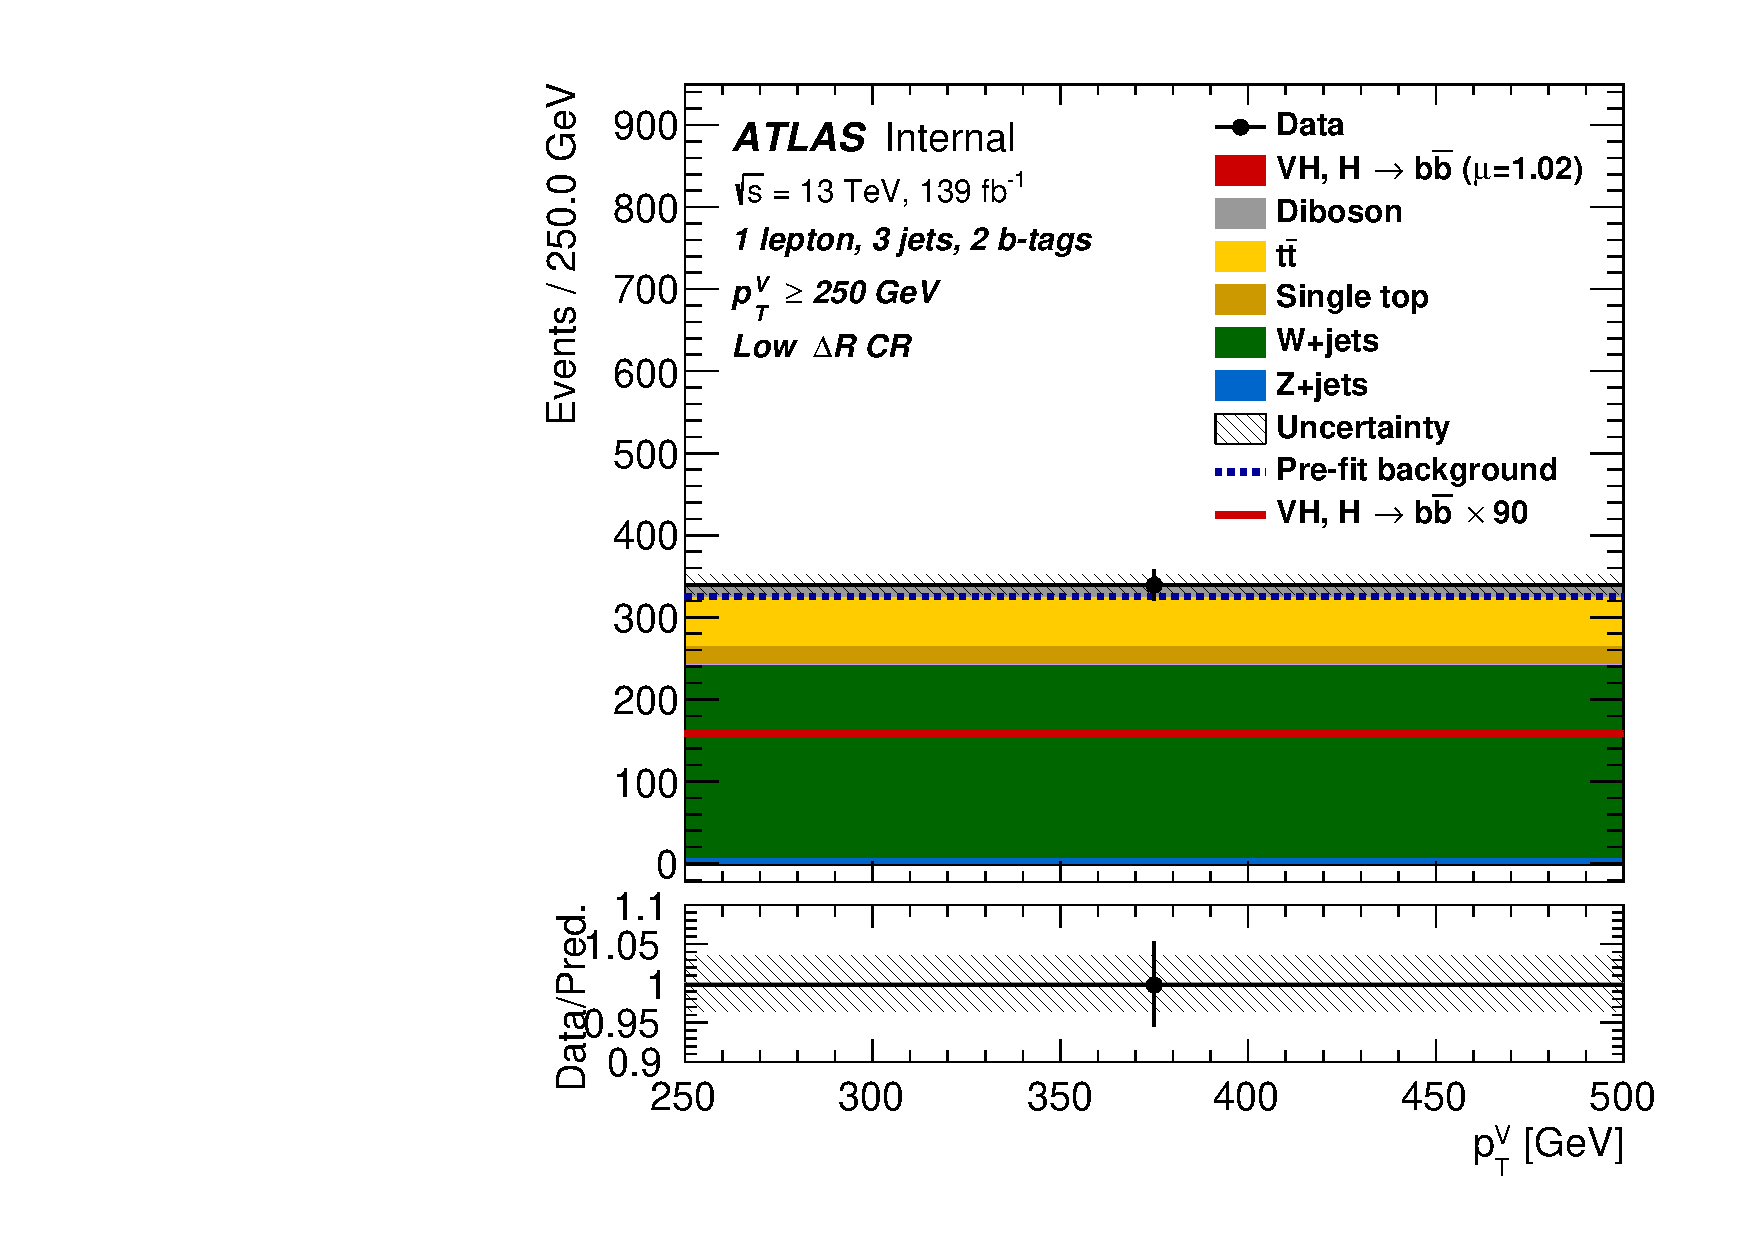
\includegraphics[width=.3\textwidth]{final_fit_mva/postfit/Region_BMin250_Y6051_DCRLow_T2_L1_distpTV_J3_GlobalFit_unconditionnal_mu1} \\
  \end{tabular}
  \caption{Post-fit distributions in the 1 lepton 3 jet channel.}
\end{figure}
\begin{figure}
  \centering
  \begin{tabular}{cc}
    % top row
    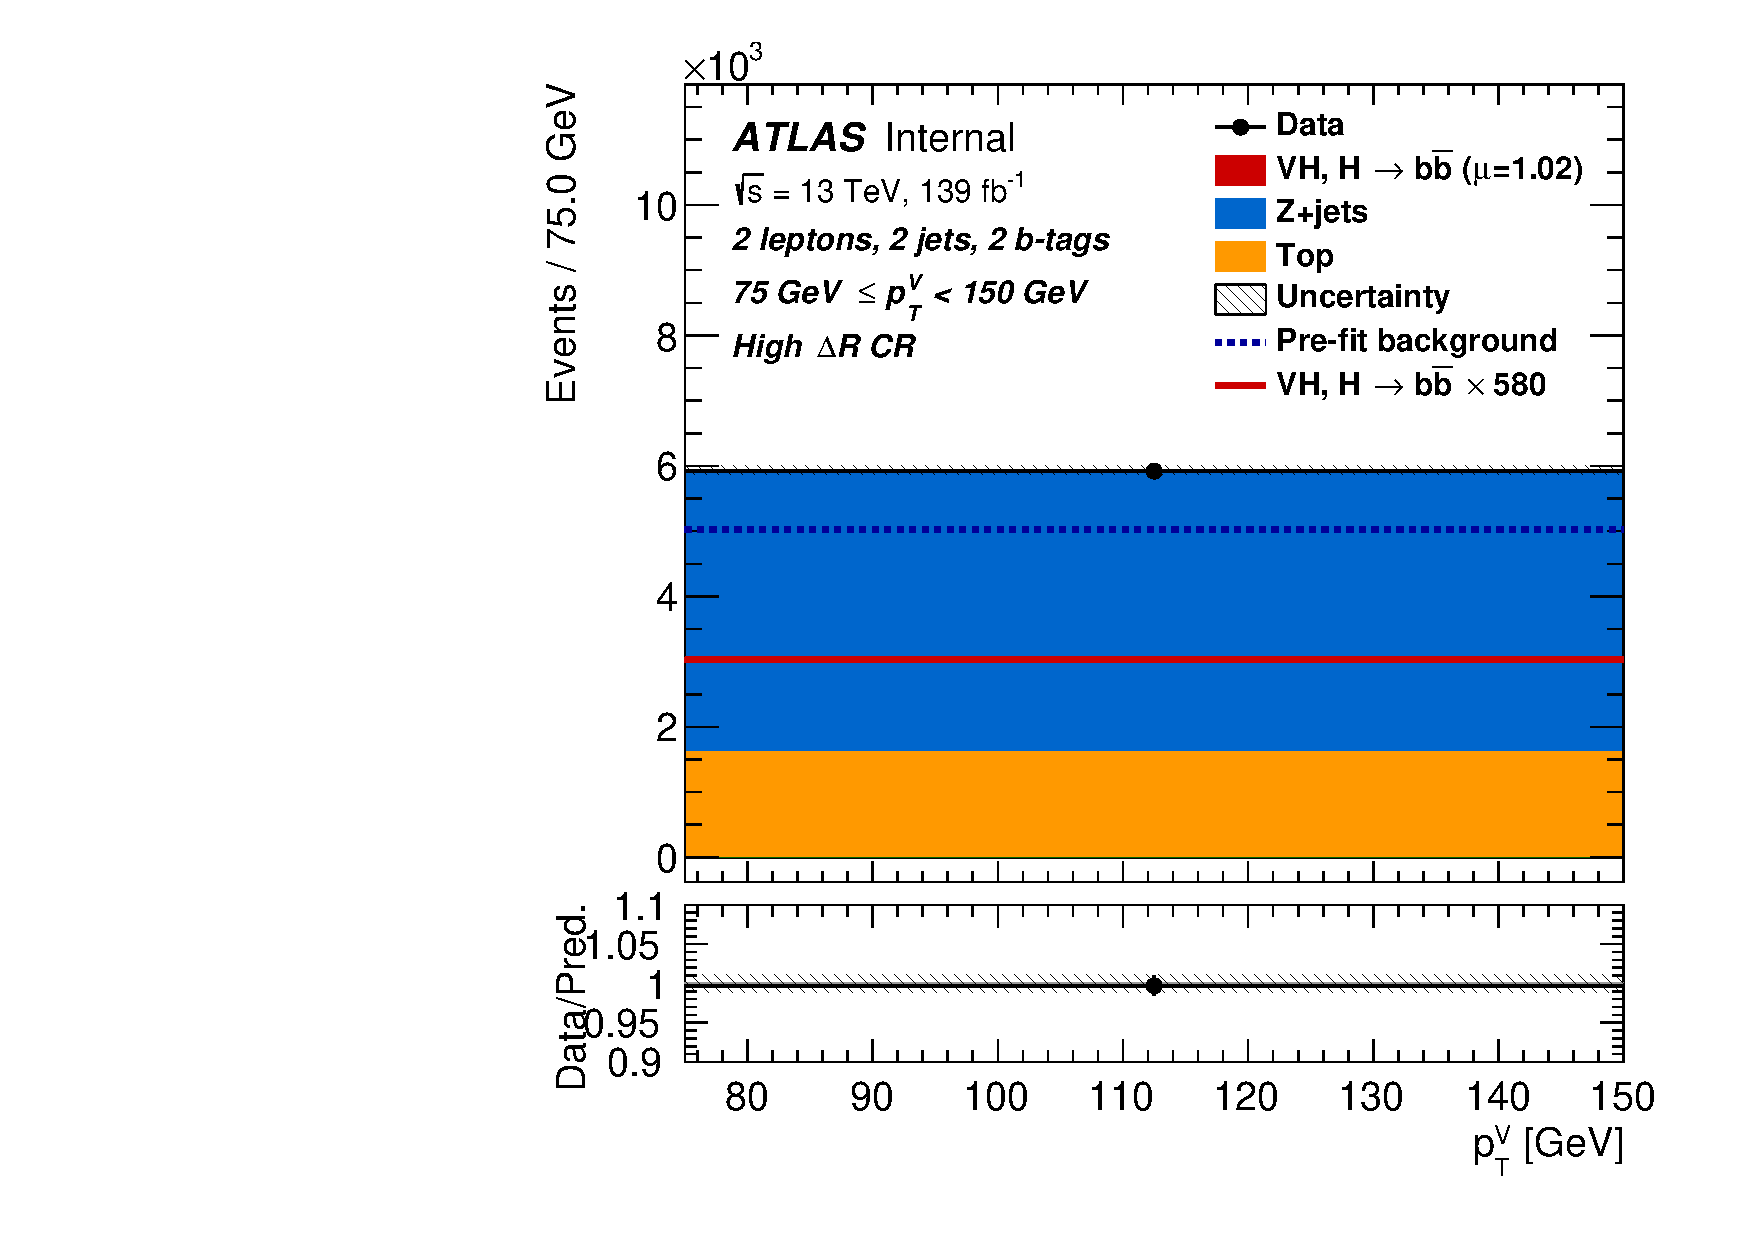
\includegraphics[width=.3\textwidth]{final_fit_mva/postfit/Region_BMax150_BMin75_Y6051_DCRHigh_T2_L2_distpTV_J2_GlobalFit_unconditionnal_mu1}%
    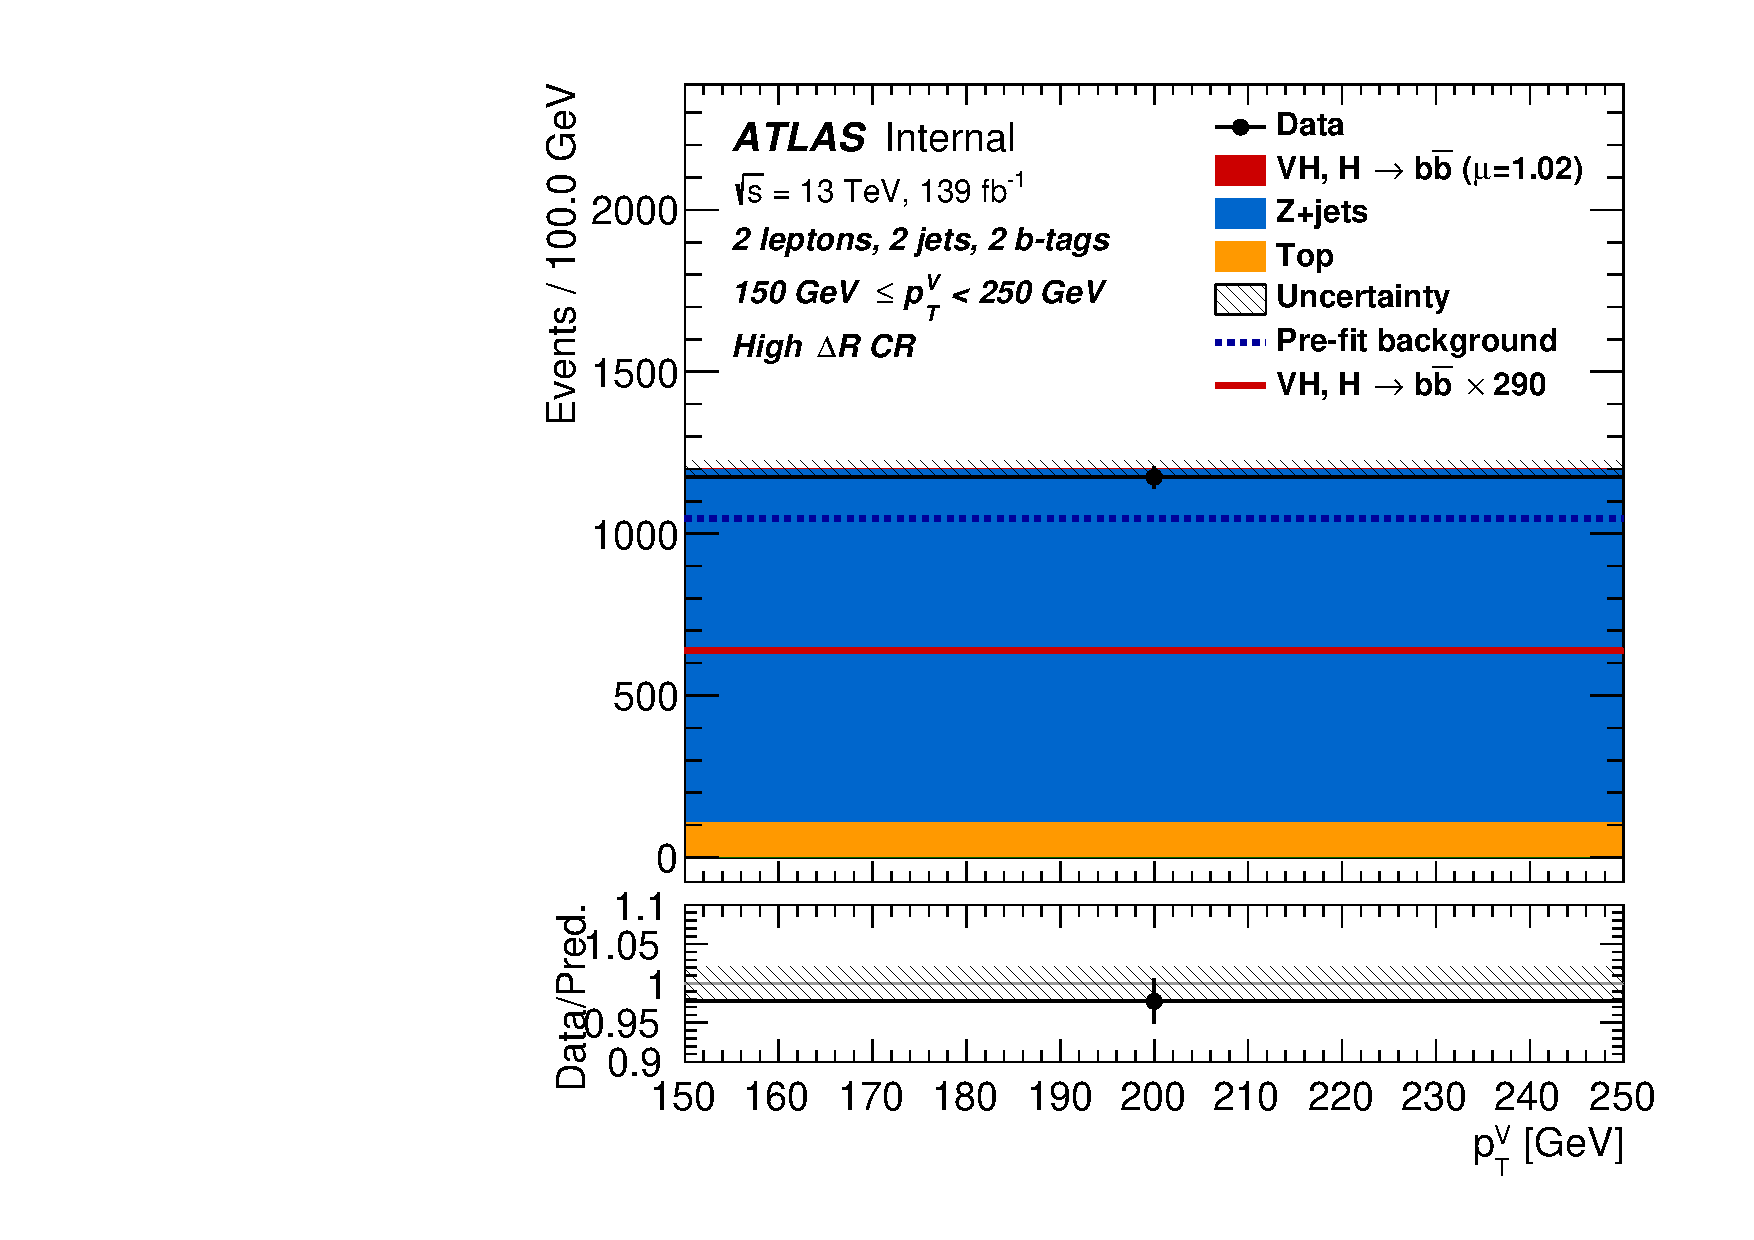
\includegraphics[width=.3\textwidth]{final_fit_mva/postfit/Region_BMax250_BMin150_Y6051_DCRHigh_T2_L2_distpTV_J2_GlobalFit_unconditionnal_mu1}%
    & 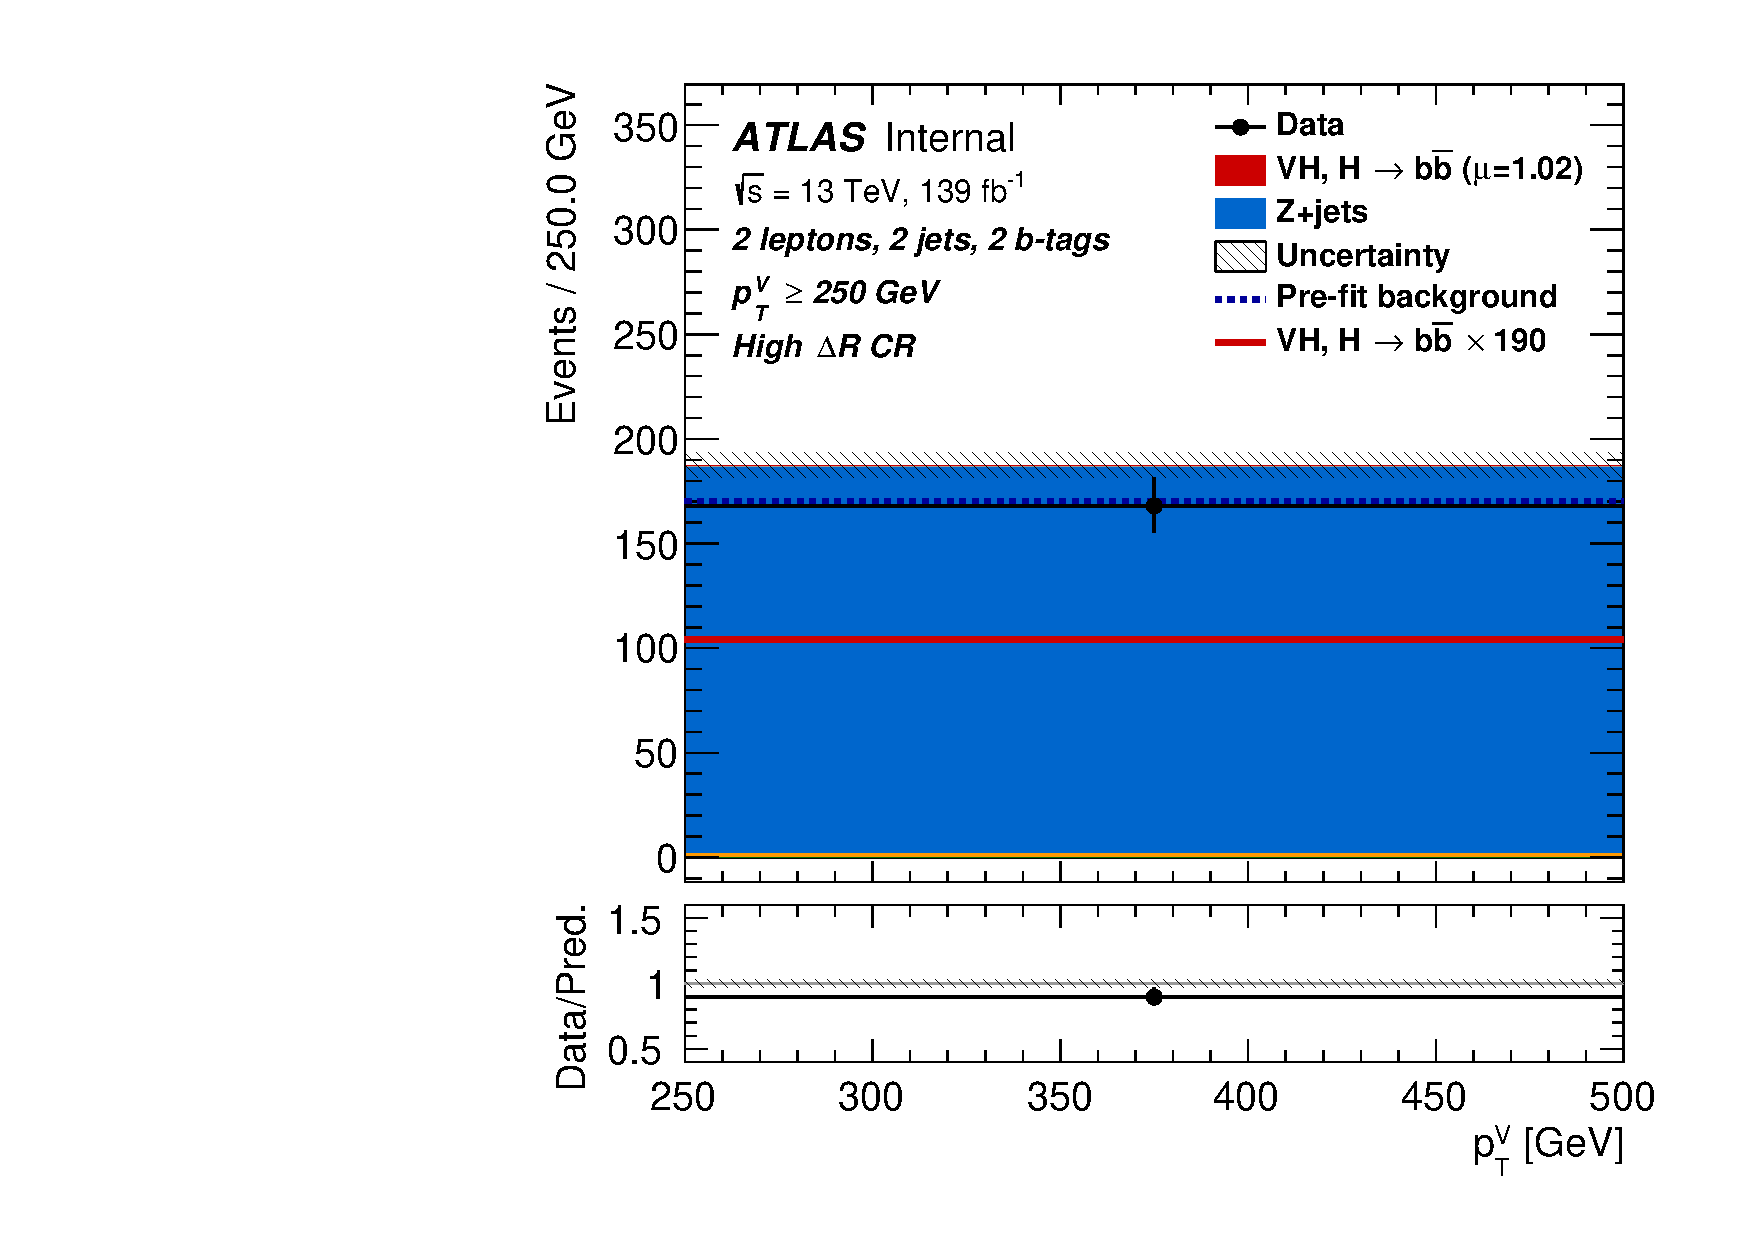
\includegraphics[width=.3\textwidth]{final_fit_mva/postfit/Region_BMin250_Y6051_DCRHigh_T2_L2_distpTV_J2_GlobalFit_unconditionnal_mu1} \\

    % middle row
    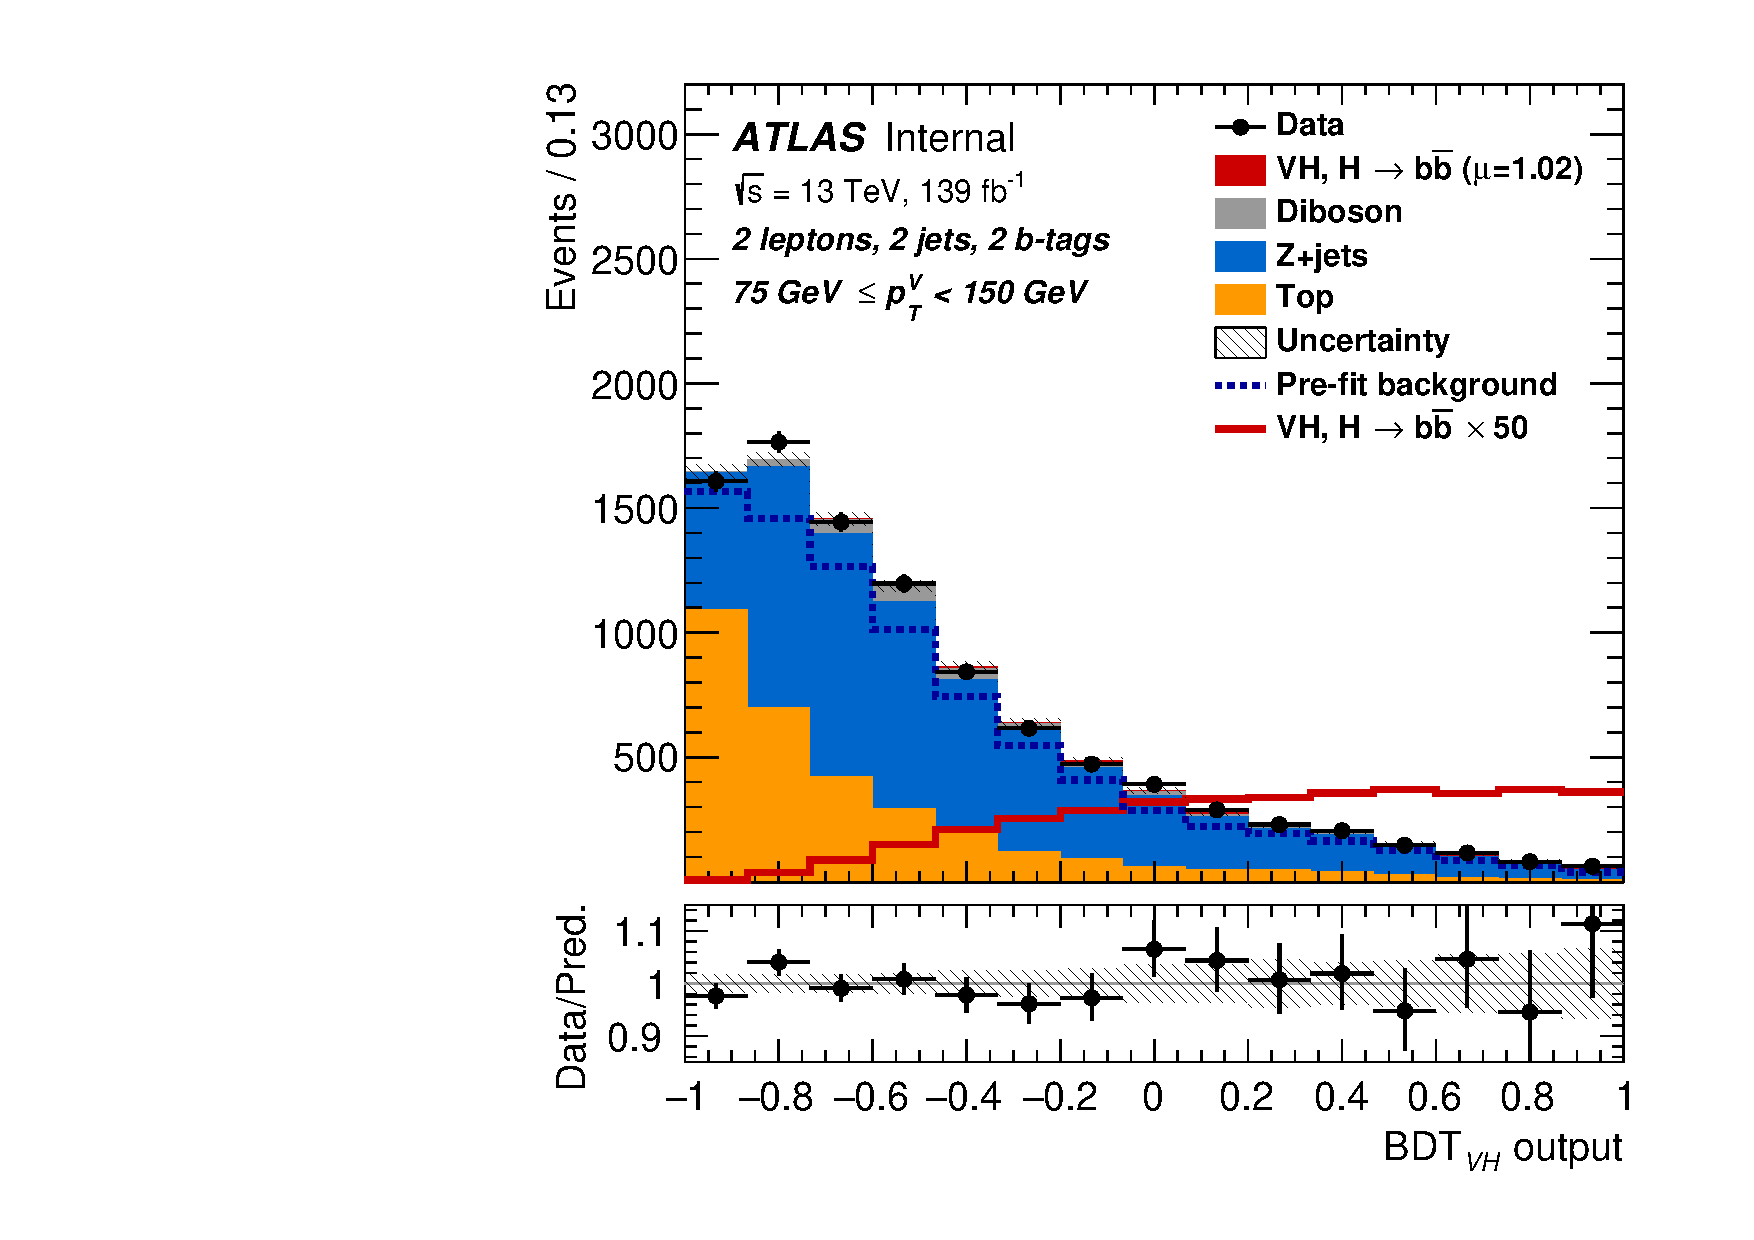
\includegraphics[width=.3\textwidth]{final_fit_mva/postfit/Region_BMax150_BMin75_Y6051_DSR_T2_L2_distmva_J2_GlobalFit_unconditionnal_mu1}%
    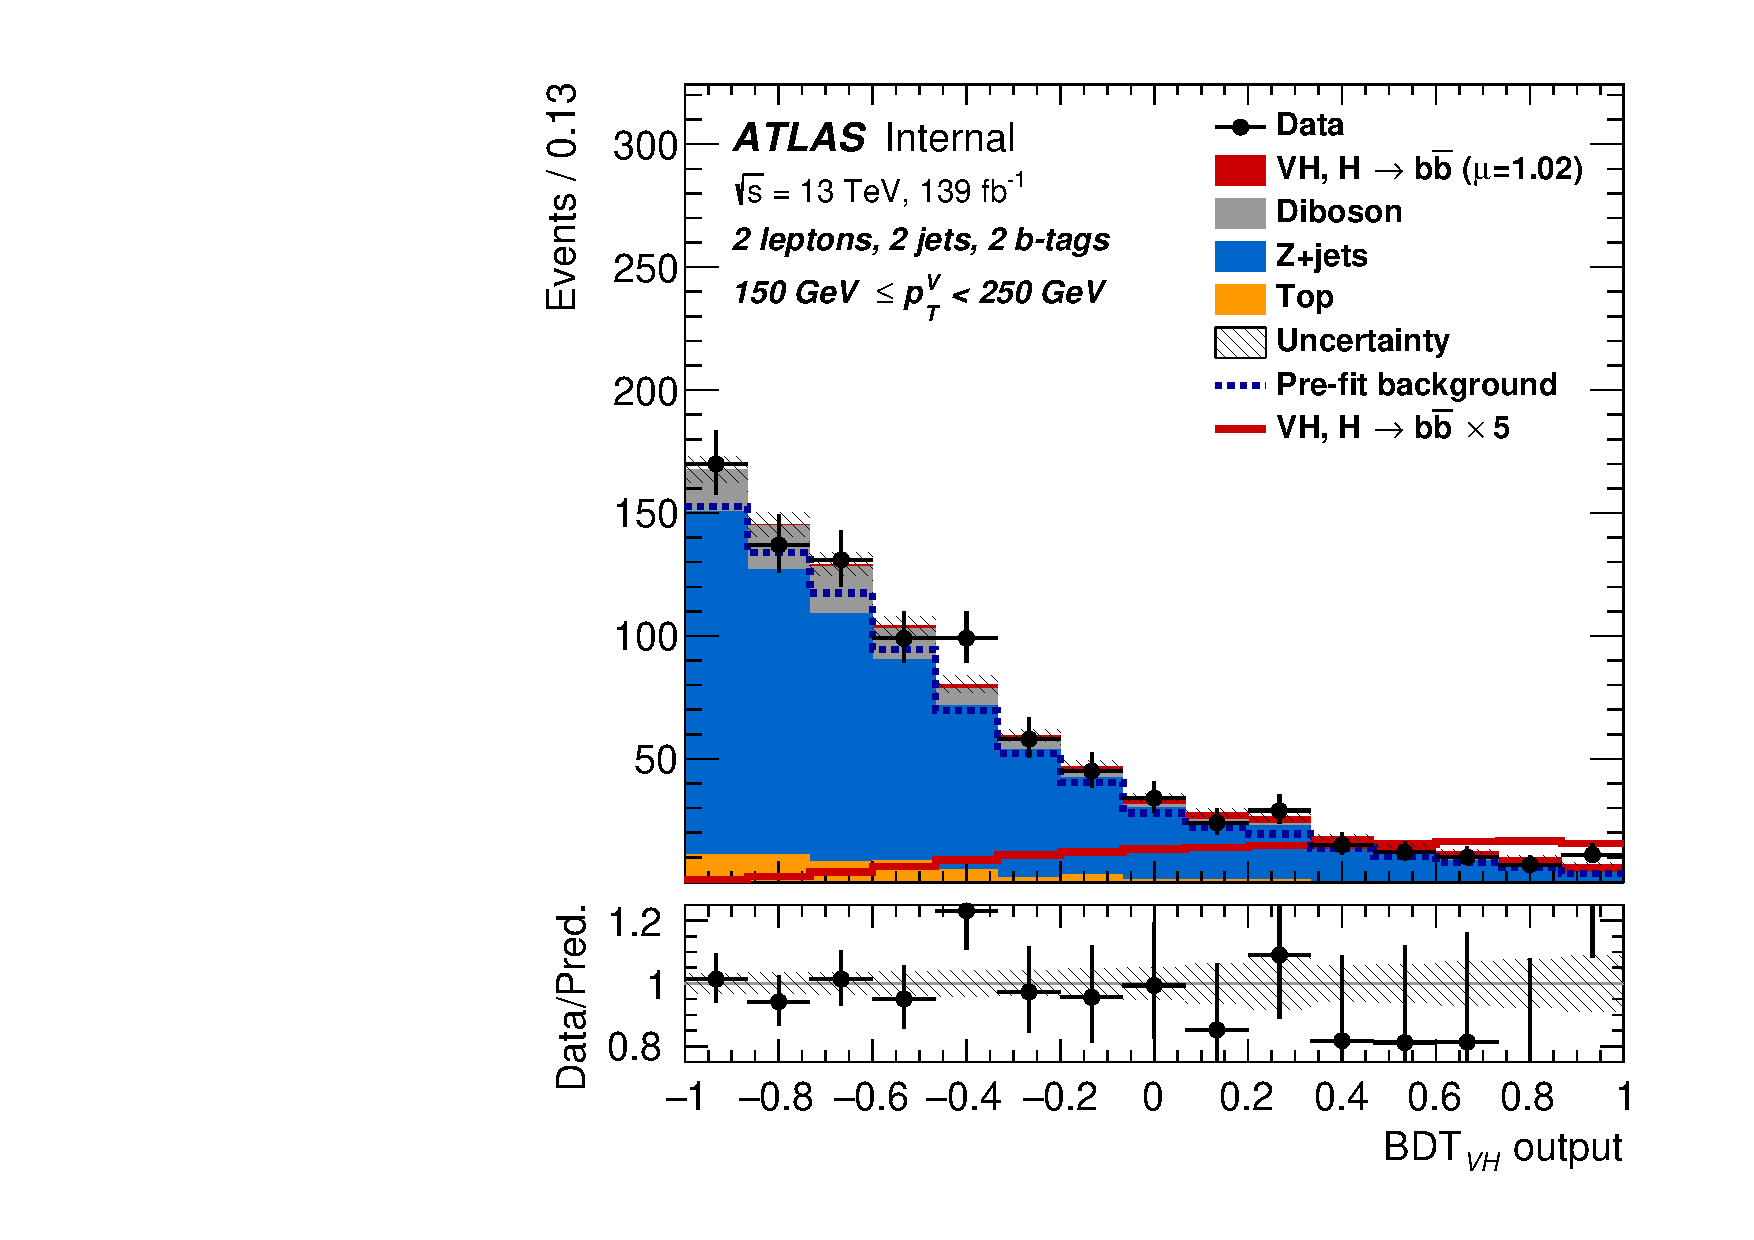
\includegraphics[width=.3\textwidth]{final_fit_mva/postfit/Region_BMax250_BMin150_Y6051_DSR_T2_L2_distmva_J2_GlobalFit_unconditionnal_mu1}%
    & 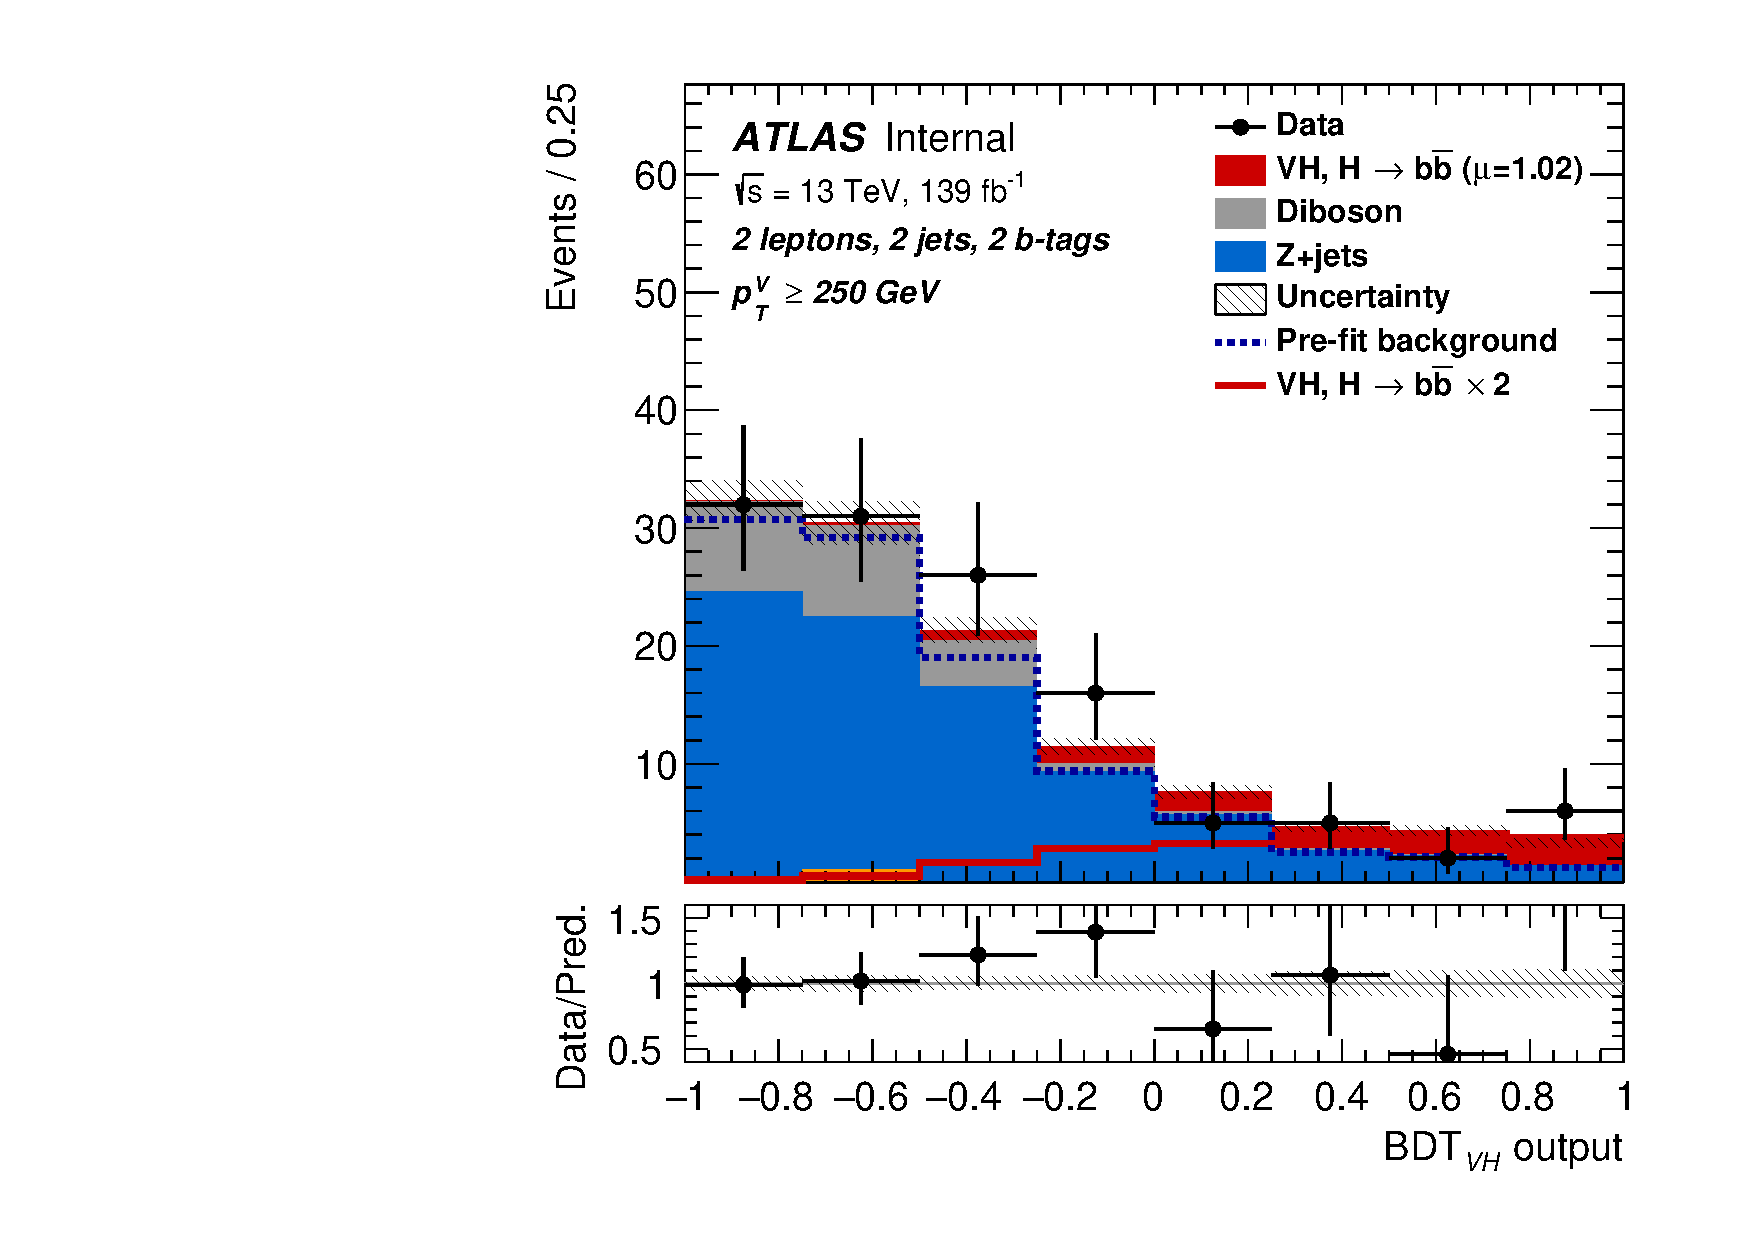
\includegraphics[width=.3\textwidth]{final_fit_mva/postfit/Region_BMin250_Y6051_DSR_T2_L2_distmva_J2_GlobalFit_unconditionnal_mu1} \\

    % bottom row
    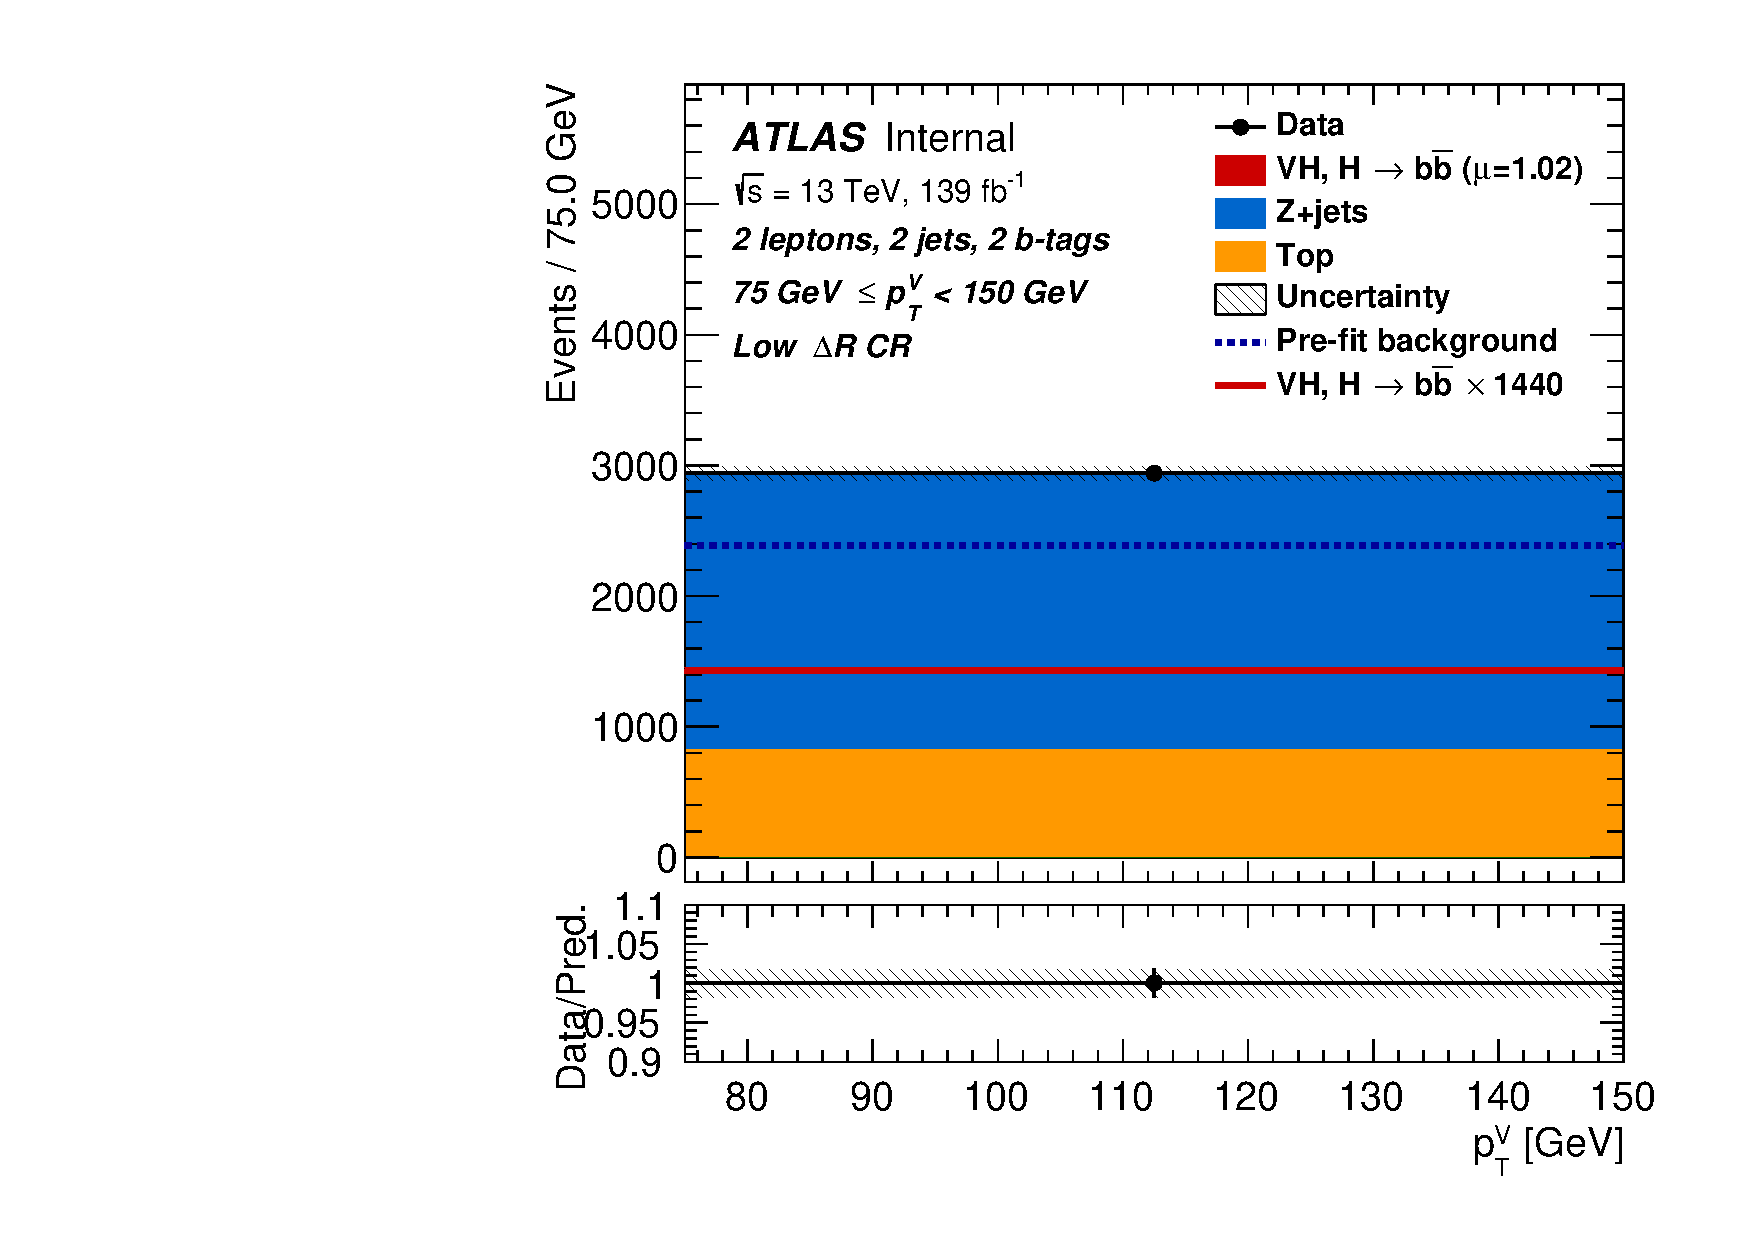
\includegraphics[width=.3\textwidth]{final_fit_mva/postfit/Region_BMax150_BMin75_Y6051_DCRLow_T2_L2_distpTV_J2_GlobalFit_unconditionnal_mu1}%
    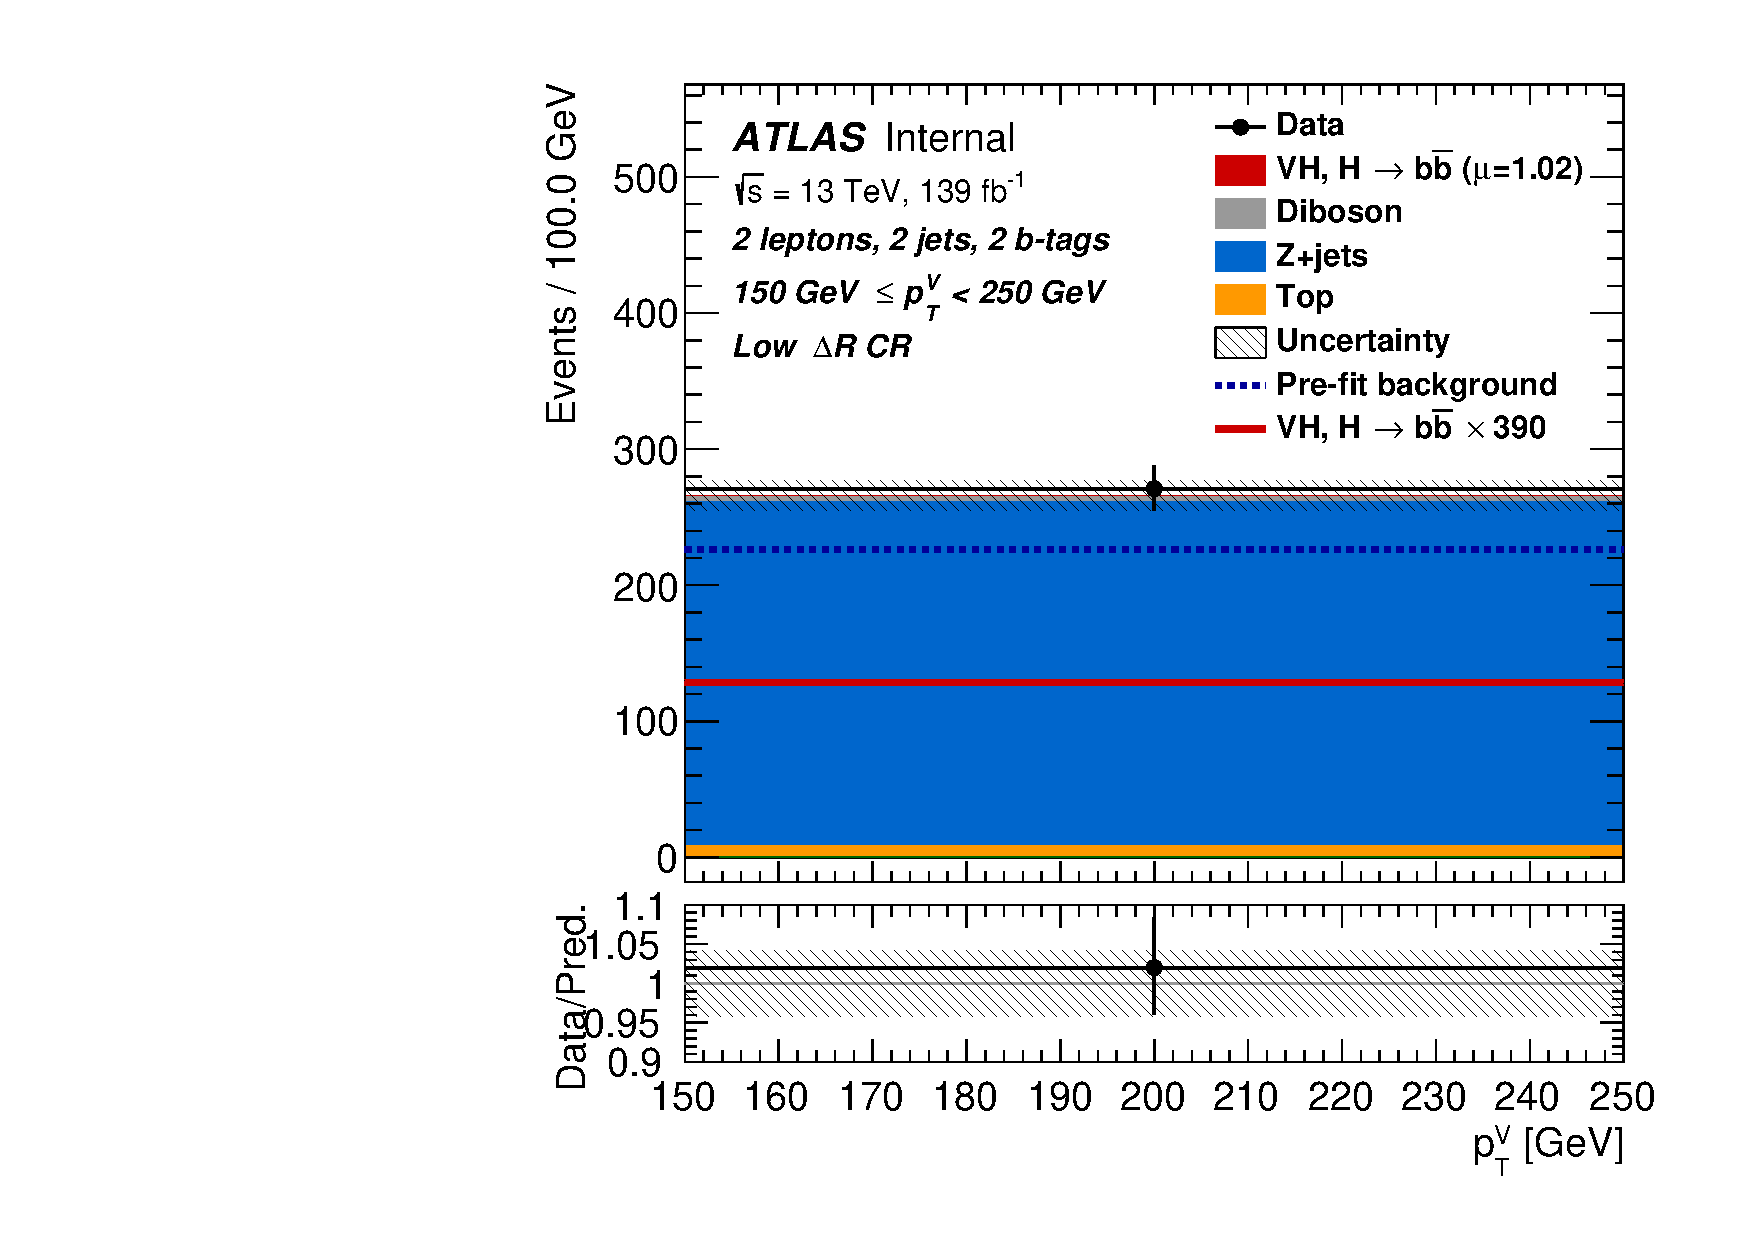
\includegraphics[width=.3\textwidth]{final_fit_mva/postfit/Region_BMax250_BMin150_Y6051_DCRLow_T2_L2_distpTV_J2_GlobalFit_unconditionnal_mu1}%
    & 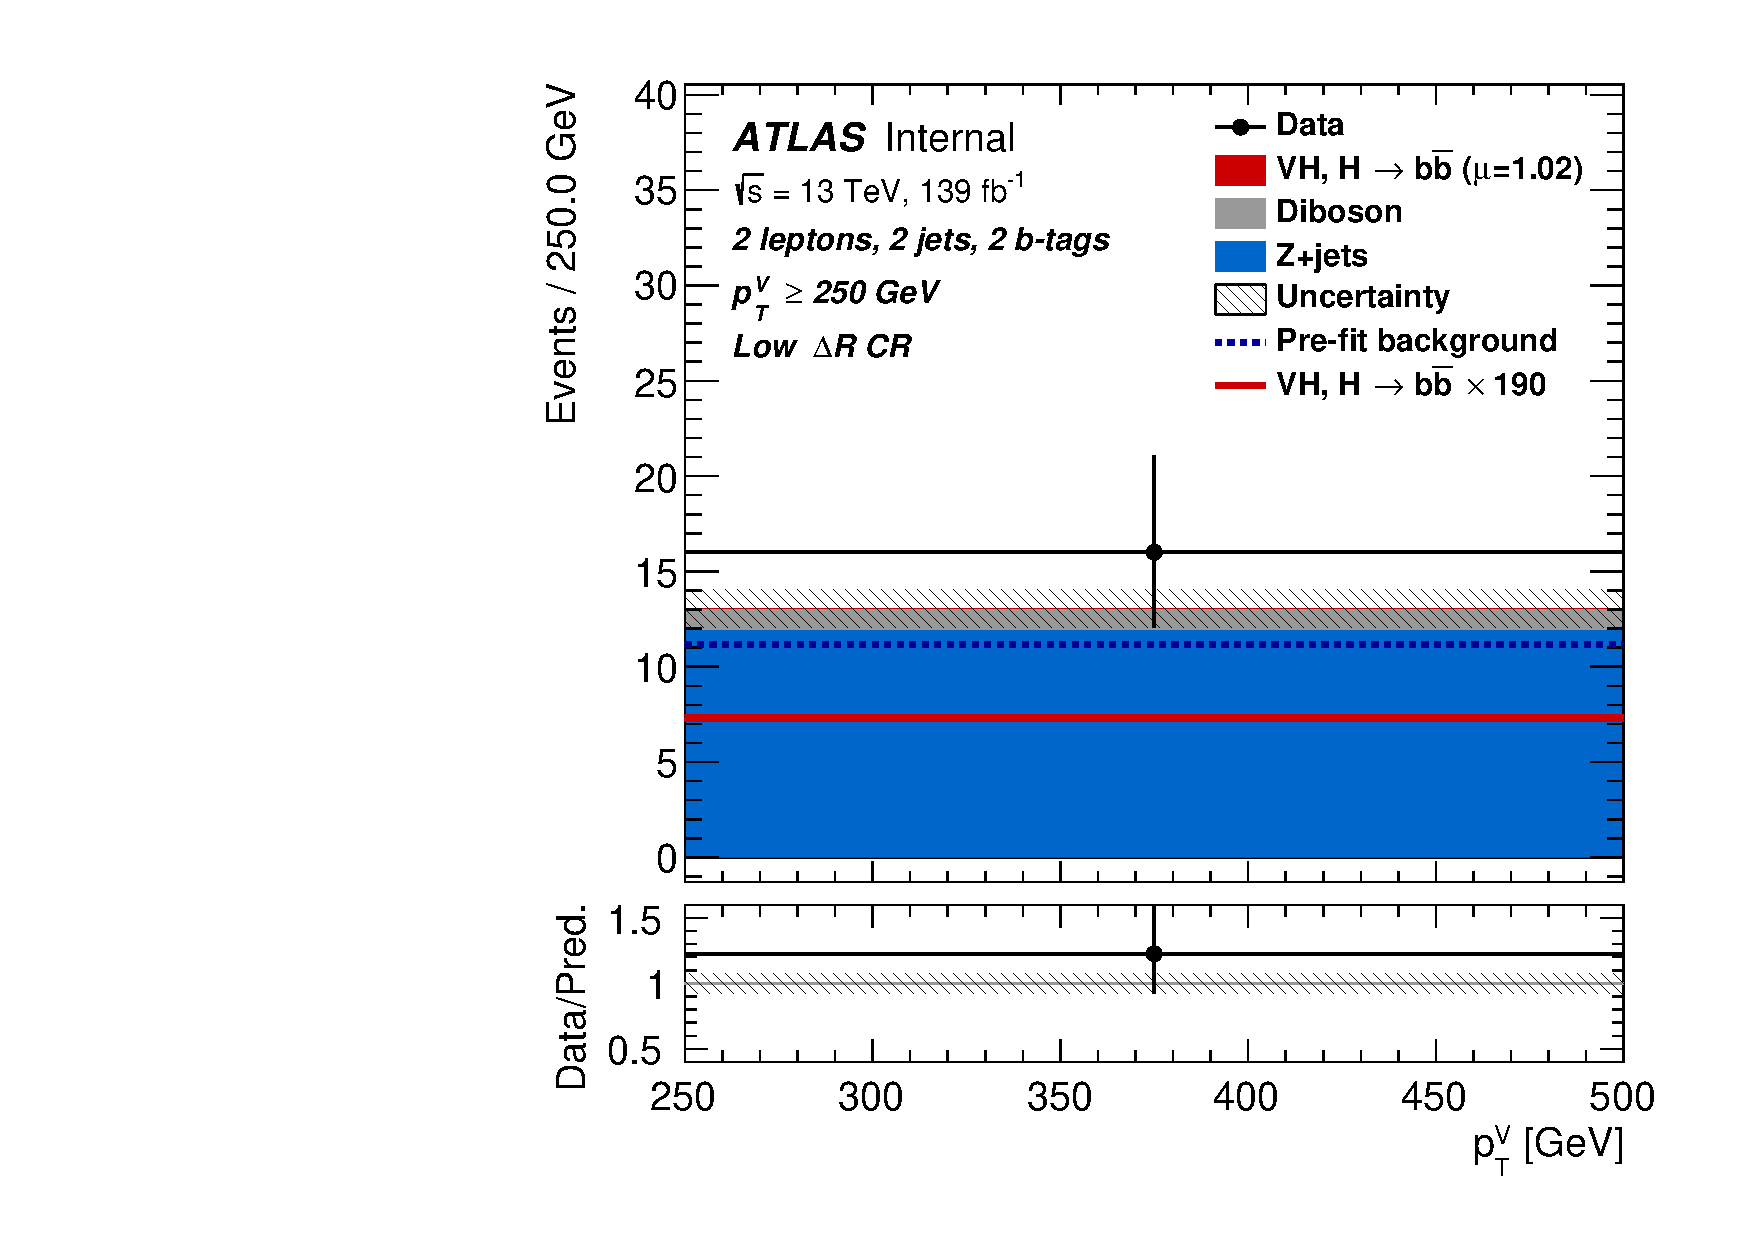
\includegraphics[width=.3\textwidth]{final_fit_mva/postfit/Region_BMin250_Y6051_DCRLow_T2_L2_distpTV_J2_GlobalFit_unconditionnal_mu1} \\
  \end{tabular}
  \caption{Post-fit distributions in the 2--lepton 2--jet channel.}
\end{figure}
\begin{figure}
  \centering
  \begin{tabular}{cc}
    % top row
    \includegraphics[width=.33\textwidth]{final_fit_mva/postfit/Region_BMax150_BMin75_incJet1_Y6051_DCRHigh_T2_L2_distpTV_J3_GlobalFit_unconditionnal_mu1}%
    \includegraphics[width=.33\textwidth]{final_fit_mva/postfit/Region_BMax250_BMin150_incJet1_Y6051_DCRHigh_T2_L2_distpTV_J3_GlobalFit_unconditionnal_mu1}%
    & \includegraphics[width=.33\textwidth]{final_fit_mva/postfit/Region_BMin250_incJet1_Y6051_DCRHigh_T2_L2_distpTV_J3_GlobalFit_unconditionnal_mu1} \\

    % middle row
    \includegraphics[width=.33\textwidth]{final_fit_mva/postfit/Region_BMax150_BMin75_incJet1_Y6051_DSR_T2_L2_distmva_J3_GlobalFit_unconditionnal_mu1}%
    \includegraphics[width=.33\textwidth]{final_fit_mva/postfit/Region_BMax250_BMin150_incJet1_Y6051_DSR_T2_L2_distmva_J3_GlobalFit_unconditionnal_mu1}%
    & \includegraphics[width=.33\textwidth]{final_fit_mva/postfit/Region_BMin250_incJet1_Y6051_DSR_T2_L2_distmva_J3_GlobalFit_unconditionnal_mu1} \\

    % bottom row
    \includegraphics[width=.33\textwidth]{final_fit_mva/postfit/Region_BMax150_BMin75_incJet1_Y6051_DCRLow_T2_L2_distpTV_J3_GlobalFit_unconditionnal_mu1}%
    \includegraphics[width=.33\textwidth]{final_fit_mva/postfit/Region_BMax250_BMin150_incJet1_Y6051_DCRLow_T2_L2_distpTV_J3_GlobalFit_unconditionnal_mu1}%
    & \includegraphics[width=.33\textwidth]{final_fit_mva/postfit/Region_BMin250_incJet1_Y6051_DCRLow_T2_L2_distpTV_J3_GlobalFit_unconditionnal_mu1} \\
  \end{tabular}
  \caption{Post-fit distributions in the 2--lepton, $\geq$3--jet channel.}
\end{figure}

\clearpage
\newpage




\subsection{Breakdown and Ranking of Uncertainties}
Show the breakdown and ranking of the uncertainties, explain briefly the physics
reasons why things appear where they do. Then later in conc. refer to how to
improve the analysis with reference to the breakdown.

\subsection{Signal Strength and STXS Measurements}
Show the signal strength measurements and STXS measurements, everything agrees
with the standard model so there is not much to state beyond that.

(+ add in chapter 6 mention the multiple POI version of the fit which yields the
STXS measurement, briefly describe what this is defining the Njet - NHjet
procedure to get the STXS bins, i.e. define the fiducial space)

